% ------------------------------------------------------------------------------
% The OpenQuake-engine Users Manual
%
% Authors:
% 	Helen Crowley 		- Executive Committee - GEM Foundation, Pavia, Italy
% 	Damiano Monelli 	- GEM Model Facility, Zurich, Switzerland
% 	Marco Pagani 		- Executive Committee - GEM Foundation, Pavia, Italy
% 	Vitor Silva 		- GEM Model Facility, Pavia, Italy
%	Graeme Weatherill - GEM Model Facility, Pavia, Italy
%  Anirudh Rao       - GEM Model Facility, Pavia, Italy
%
% License:
% Document distributed under the CC BY-NC-SA 4.0 License
% Creative Commons Attribution-NonCommercial-ShareAlike 4.0 International
% http://creativecommons.org/licenses/by-nc-sa/4.0/
%
% Copyright:
% © GEM Foundation, Pavia, Italy. 2013--2015.
% ------------------------------------------------------------------------------

%-------------------------------------------------------------------------------
%  PACKAGES AND OTHER DOCUMENT CONFIGURATIONS
%-------------------------------------------------------------------------------

\documentclass[11pt,fleqn]{book} % ------------------ Left-justified equations -
%%%%%%%%%%%%%%%%%%%%%%%%%%%%%%%%%%%%%%%%%%%%%%%%%%%%%%%%%%%%%%%%%%%%%%%%%%%%%%%%
% The GEM Technical Documentation LaTeX Template
% Version 1.0 (12/4/14)
%
% Original author:
% Mathias Legrand (legrand.mathias@gmail.com)
%
% Adapted for use by the GEM Foundation by:
% James Brown (james.brown@globalquakemodel.org)
% Anirudh Rao (anirudh.rao@globalquakemodel.org)
%
% License:
% CC BY-NC-SA 3.0 (http://creativecommons.org/licenses/by-nc-sa/3.0/)
%
% Compiling this template:
% This template uses bibtex for its bibliography and makeindex for its index.
% When you first open the template, compile it from the command line with the
% commands below to make sure your LaTeX distribution is configured correctly:
%
% 1) pdflatex -interaction=nonstopmode oq-manual.tex
% 2) bibtex oq-manual
% 3) pdflatex -interaction=nonstopmode oq-manual.tex
% 4) pdflatex -interaction=nonstopmode oq-manual.tex
% 5) makeindex oq-manual.idx -s configuration/StyleInd.ist
% 6) makeglossaries oq-manual
% 7) pdflatex -interaction=nonstopmode oq-manual.tex
%
% After this, when you wish to update the bibliography/index use the appropriate
% command above and make sure to compile with pdflatex several times
% afterwards to propagate your changes to the document.
%
% This template also uses a number of packages which may need to be
% updated to the newest versions for the template to compile. It is strongly
% recommended you update your LaTeX distribution if you have any
% compilation errors.
%
% Important note:
% Chapter heading images should have a 2:1 width:height ratio,
% e.g. 920px width and 460px height.
%
%%%%%%%%%%%%%%%%%%%%%%%%%%%%%%%%%%%%%%%%%%%%%%%%%%%%%%%%%%%%%%%%%%%%%%%%%%%%%%%%

% Page layout and margins
\usepackage[top=3cm,bottom=3cm,left=3.2cm,right=3.2cm,headsep=10pt,a4paper]{geometry}
\linespread{1.25}

% Font settings
\usepackage[condensed]{roboto} % Use the Roboto font for headings
\usepackage[bitstream-charter]{mathdesign} % Use the Bitstream Charter font for text
% \usepackage{amsmath,amsfonts,amssymb,amsthm} % For math equations, theorems, symbols, etc
\usepackage{microtype} % Slightly tweak font spacing for aesthetics
\usepackage[utf8]{inputenc} % Required for including letters with accents
\usepackage[T1]{fontenc} % Use 8-bit encoding that has 256 glyphs

% Color settings
\usepackage{color, colortbl}
\usepackage{xcolor} % Required for specifying colors by name
\definecolor{oqblue}{RGB}{27,117,165} % From the GEM Brand Guidelines
\definecolor{darkblue}{rgb}{.2,.2,.8}
\definecolor{darkgray}{gray}{0.25}

% Bibliography settings
\usepackage{csquotes}
\usepackage[style=alphabetic,
            sorting=nyt,
            sortcites=true,
            natbib=true,
            style=authoryear,
            maxcitenames=2,
            maxbibnames=100,
            autopunct=true,
            autolang=hyphen,
            hyperref=true,
            doi=true,
            abbreviate=false,
            backref=true,
            backend=bibtex,
            bibencoding=ascii,
            firstinits=true,
	    	uniquename=false,
	    	uniquelist=false]{biblatex}
\addbibresource{bibliography/hazard.bib} % Hazard BibTeX bibliography file
\addbibresource{bibliography/risk.bib} % Risk BibTeX bibliography file
\defbibheading{bibempty}{}

% Figure caption settings
\usepackage[textfont=it,margin=10pt,font=small,labelfont=bf,labelsep=endash]{caption}
\usepackage{subcaption}

% Rotate any object
\usepackage{rotating}

% Verbatim environments
\usepackage{verbatim}
\usepackage{fancyvrb}

% Index settings
\usepackage{calc} % Infix notation for \setcounter, \addtocounter, \setlength, \addtolength
\usepackage{makeidx} % Required to make an index
\setcounter{secnumdepth}{3}
\setcounter{tocdepth}{3} % Entries down to \subsubsections in the TOC
\makeindex % Tells LaTeX to create the files required for indexing

\usepackage{todonotes}
\usepackage{marginnote}

% Access bold symbols in maths mode
\usepackage{bm}

% Flexible typesetting of tables and figures
\usepackage{ctable}
\usepackage{booktabs}

% Customization of section titles and table of contents
\usepackage{titlesec}
\usepackage{titletoc}

% Header and footer customization
\usepackage{fancyhdr}
\usepackage{etoolbox}

\usepackage{graphicx} % Required for including pictures
\usepackage{tikz} % Required for drawing custom shapes
\usepackage{eso-pic} % Required for specifying an image background in the title page
\usepackage{pdfpages} % Needed to load .pdf pages, used for the cover page

% English language hyphenation
\usepackage[english]{babel}

\usepackage{enumitem} % Customize lists
\setlist{nolistsep} % Reduce spacing between bullet points and numbered lists
\usepackage{listings} % Required for embedding code snippets

\usepackage{hyperref}
\hypersetup{hidelinks,colorlinks=true,breaklinks=true,citecolor=darkblue,linkcolor=darkgray,urlcolor=oqblue,bookmarksopen=false,pdftitle={Title},pdfauthor={Author}}

% Package to create a glossary - must be loaded after hyperref
\usepackage[acronym,nonumberlist,style=altlist]{glossaries}
\glstoctrue
\makeglossaries


 % ------------- Load packages and template -
\graphicspath{{figures/}} % -------------- Directory where pictures are stored -

\begin{document}
\input{oqum/glossary} % ---------------------------------------- Load glossary -

%-------------------------------------------------------------------------------
%  COVER PAGE
%-------------------------------------------------------------------------------

\includepdf[pages=-]{figures/oq_manual_cover.pdf}

%-------------------------------------------------------------------------------
%  TITLE PAGE
%-------------------------------------------------------------------------------

\begingroup
\thispagestyle{empty}
\begin{center}
\par\normalfont\fontsize{15}{15}\sffamily\selectfont
\textcolor{oqblue}{OpenQuake: calculate, share, explore}
\vspace*{9cm}
\par\bfseries\fontsize{35}{35}\sffamily\selectfont
\textcolor{gembrown}{The OpenQuake-engine\\User Instruction Manual}\par
\vspace*{9cm}
\par\normalfont\fontsize{15}{15}\sffamily\selectfont
\href{http://globalquakemodel.org/openquake/}{\textcolor{oqblue}{globalquakemodel.org/openquake}}
\end{center}
\endgroup

%-------------------------------------------------------------------------------
%  COPYRIGHT PAGE
%-------------------------------------------------------------------------------

\newpage
~\vfill
\thispagestyle{empty}

\noindent
   \textbf{Authors} \\
   Helen Crowley$^1$, Damiano Monelli$^2$, Marco Pagani$^1$, Vitor Silva$^3$,
   Graeme Weatherill$^3$, Anirudh Rao$^3$ \hfill \\
   \hfill \\
   \small
   \begin{tabular}{p{4cm}p{4cm}p{4cm}}
   $^1$ GEM Foundation \hfill \newline
   via Ferrata, 1 \hfill \newline
   20133 Pavia \hfill \newline
   Italy \hfill \newline
   &
   $^2$ GEM Model Facility \hfill \newline
   SED - ETHZ \hfill \newline
   Sonneggstrasse, 5 \hfill \newline
   CH-8092 Zurich\hfill \newline
   Switzerland \hfill \newline
   &
   $^3$ GEM Model Facility \hfill \newline
   via Ferrata, 1 \hfill \newline
   20133 Pavia \hfill \newline
   Italy \hfill \newline
   \end{tabular} \hfill \newline
   %
   Email address for all the authors:\hfill\\
   $<$name.surname$>$@globalquakemodel.org\hfill\\
   \normalsize

\noindent
   {\textbf{Citation}} \hfill \\
   Please cite this document as: \hfill \\
   Crowley, H., Monelli, D., Pagani, M., Silva, V., Weatherill, G.,
   and Rao, A. (2015). The OpenQuake-engine User Manual.
   \textit{Global Earthquake Model (GEM) Technical Report 2015-11.\\
   doi: 10.13117/GEM.OPENQUAKE.MAN.ENGINE.1.6/01, 148 pages.} \hfill \\
\noindent \hfill\\
\noindent
   {\bf{Disclaimer}} \hfill \\
   The OpenQuake-engine User Manual is distributed in the hope that it will be
   useful, but without any warranty: without even the implied warranty of
   merchantability or fitness for a particular purpose. While every precaution
   has been taken in the preparation of this document, in no event shall the
   authors of the Manual and the GEM Foundation be liable to any party for
   direct, indirect, special, incidental, or consequential damages, including
   lost profits, arising out of the use of information contained in this
   document or from the use of programs and source code that may accompany it,
   even if the authors and GEM Foundation have been advised of the possibility
   of such damage. The Manual provided hereunder is on as ``as is'' basis, and
   the  authors and GEM Foundation have no obligations to provide maintenance,
   support, updates, enhancements, or modifications. \hfill \\
\noindent \hfill\\
\noindent
   {\bf{License}} \hfill \\
   This Manual is distributed under the Creative Commons License  Attribution-
   NonCommercial-ShareAlike 4.0 International
   (\href{http://creativecommons.org/licenses/by-nc-sa/4.0/} {CC BY-NC-SA
   4.0}). You can download this Manual and share it with others as long as you
   provide proper credit, but you cannot change it in any way or use it
   commercially.\hfill \\

\noindent \copyright\ \textsc{2013--2015 GEM Foundation}\\
\noindent \textit{Sixth printing, November 2015} % Printing/edition date

%-------------------------------------------------------------------------------
%  TABLE OF CONTENTS
%-------------------------------------------------------------------------------

\chapterimage{figures/chapter_head_1.pdf} % Table of contents heading image
\pagestyle{empty} % No headers
\tableofcontents % Print the table of contents itself
\cleardoublepage % Forces the first chapter to start on the right
\pagestyle{fancy} % Print headers again

%-------------------------------------------------------------------------------
%  FOREWORD
%-------------------------------------------------------------------------------
\chapterimage{figures/chapter_head_2.pdf} % Chapter heading image
\chapter*{Preface}
\addcontentsline{toc}{chapter}{Preface}
\input{oqum/preamble}

%-------------------------------------------------------------------------------
%  THE MANUAL
%-------------------------------------------------------------------------------

% ------------------------------------------------------- Part I: Introduction -
\part{Introduction}
\label{part:introduction}
\chapterimage{figures/chapter_head_2.pdf} % Chapter heading image
\chapter{OpenQuake-engine Background}
	\glsdesc{acr:oqe} is the seismic hazard and risk calculation software developed by
the \glsdesc{acr:gem}. By following current standards in software
developments like test-driven development and continuous integration, the
\glsdesc{acr:oqe} aims at becoming an open, and community-driven tool for
seismic hazard and risk analysis.

The source code of the \glsdesc{acr:oqe} is available on a public web-based
repository at the following address:

\href{http://github.com/gem/oq-engine}{http://github.com/gem/oq-engine}.


% ------------------------------------------------------------------------------
\section{Running the OpenQuake-engine}
\index{Running OpenQuake!introduction}
\label{sec:running_oq_engine}

An \gls{acr:oqe} analysis is launched from the command line of a terminal.

A schematic list of the options that can be used for the execution of the
\gls{acr:oqe} can be obtained with the following command:

\begin{minted}[fontsize=\footnotesize,frame=single,bgcolor=lightgray]{shell-session}
user@ubuntu:~\$ oq-engine --help
\end{minted}

The result is the following:

\inputminted[firstline=1,fontsize=\footnotesize,frame=single]{shell-session}{oqum/help.txt}\\

% ------------------------------------------------------------------------------
\section{Concurrent Computing with OpenQuake}
\label{sec:concurrent_tasks}

The \glsdesc{acr:oqe} supports concurrent computing on both standalone
computers and computer clusters.

The \glsdesc{acr:oqe} works by splitting a computation into a number of tasks
which are then processed in parallel. The user has the ability to control the
splitting procedure, at least to a certain extent, by setting the parameter
`concurrent\_tasks` in the job.ini file. The \glsdesc{acr:oqe} will try to
produce a number of tasks close to `concurrent\_tasks`: it could be more, it
could be less. The details of the algorithm used can change depending on the
release of the engine and this is why they are not documented here. Instead,
we will document how you can set the parameter to a sensible value.

For instance, suppose you have a standard PC with an i7 processor with 8
hyperthreaded cores, i.e. 4 real cores. You could set:

concurrent\_tasks = 16

and then each hyperthreaded core would process around 2 tasks, which is a
reasonable value. If your computation consumes a lot of memory, you could
increase `concurrent\_tasks`, thus producing more tasks of smaller size,
requiring less memory.

If you don't set the parameter, a default value is used. Currently the default
is set to 8 times the number of cores in your controller machine. This default
value for `concurrent\_tasks` is likely to change in the future and you should
not rely on it if you are using a computer cluster. If you are not using a
cluster, the default value should be a reasonable choice.

Now, suppose you have have a cluster with a controller node and 10 workers,
each of which has 8 hyperthreaded cores, making for 80 cores in total. In this
scenario you could set:

concurrent\_tasks = 160

If you did not set the parameter, the default (assuming 8 cores on the
controller machine) would be 8 * 8 = 64 tasks, which is not enough. The number
of available cores on the workers is 80, so 16 cores will remain unused. Our
suggestion is to provide a value:

concurrent\_tasks = 2 * number of (hyperthread) cores in the workers

or more, if the computation has memory issues. With more tasks, less memory is
used, but more data is transferred and the computation becomes slower.

If `concurrent\_tasks` is set to zero, the parallelization is disabled and the
job is executed by using a single core. This is useful when debugging errors.


% ----------------------------------------------------- Part II: Hazard Module -
\thispagestyle{empty}
\part{Hazard}

\chapterimage{figures/chapter_head_2.pdf} % Chapter heading image
\chapter{Introduction to the Hazard Module}
   \label{chap:hazintro}
	\index{OpenQuake-engine!risk}

The seismic risk results are being calculated using the OpenQuake risk library
(oq-risklib), an open-source suite of tools for seismic risk assessment and
loss estimation. This library is written in the Python programming language
and available in the form of a ``developers'' release, that can be executed
through a command line interface. The code of the library can be found on a
public repository at GitHub at the following address
\href{http://github.com/gem/oq-risklib}{http://github.com/gem/oq-risklib}.

The risk component of the OpenQuake-engine can compute both scenario-based and
probabilistic seismic damage and risk using various approaches. The following
types of analysis are currently supported:

\begin{itemize}

    \item \textit{Scenario Damage Assessment}, allowing the calculation of
	damage distribution statistics for a portfolio of buildings from a single
	earthquake rupture scenario taking into account aleatory and epistemic
	ground-motion variability.

	\item \textit{Scenario Risk Assessment}, for the calculation of individual 
	asset and portfolio loss statistics due to a single earthquake 
	rupture scenario taking into account aleatory and epistemic ground-motion 
	variability. Correlation in the vulnerability of different assets of the 
	same typology can also be taken into consideration.

	\item \textit{Classical Probabilistic Seismic Damage Analysis}, for 
	calculation of damage state probabilities over a specified time period,  
	and probabilistic collapse maps, starting from the hazard curves 
	computed following the classical integration procedure (\cite{cornell1968}, 
	\citet{mcguire1976}) as formulated by \cite{field2003}.

    \item \textit{Classical Probabilistic Seismic Risk Analysis}, allowing
	calculation of loss curves and loss maps, starting from the hazard curves 
	computed following the classical integration procedure (\cite{cornell1968}, 
	\citet{mcguire1976}) as formulated by \cite{field2003}.

	\item \textit{Event-Based Probabilistic Seismic Risk Analysis}, 
	allowing calculation of event-loss tables starting from stochastic event sets.
	Other results such as loss-exceedance curves, probabilistic loss maps, 
	average annual losses, and insured loss statistics can be obtained by post-
	processing the event-loss tables.

	\item \textit{Retrofit Benefit-Cost Ratio Analysis}, which is useful in 
	estimating the net-present value of the potential benefits of performing  
	retrofitting for a portfolio of assets (in terms of decreased losses in 
	seismic events), measured relative to the upfront cost of retrofitting.

\end{itemize}

Each calculation workflow has a modular structure, so that intermediate
results can be exported and analyzed. Moreover, each calculator can be
extended independently of the others so that additional calculation options
and methodologies can be easily introduced, without affecting the overall
calculation workflow.

The following sections describe the basic inputs required for a risk
calculation, including exposure models, fragility models, consequence models,
and vulnerability models. The final section of this chapter describes each of
the above workflows in detail.

For further information regarding the theoretical background of the
methodologies used for each calculator, users are referred to the OpenQuake-
engine Book (Risk).


\section{Exposure models}
\label{sec:exposure}
All risk calculators in the OpenQuake-engine require an \gls{exposure model}
that needs to be provided in the NRML format. The information included in an
exposure model comprises a metadata section, followed by data regarding each
individual asset in the portfolio.

There are a number of parameters that compose the metadata, and provides
general information regarding the \glspl{asset} within the \gls{exposure
model}, as described below:

\begin{itemize}

    \item \Verb+id+: a unique key used to identify the gls{exposure model};

    \item \Verb+category+: a string used to define the type of glspl{asset}
    being stored (e.g: buildings, lifelines);

    \item \Verb+taxonomySource+: attribute used to define the gls{taxonomy}
    being used to classify the glspl{asset};

    \item \Verb+description+: brief string with further information about the
    \gls{exposure model};

\end{itemize}

The information in the metadata section is common to all of the assets in the
portfolio and needs to be incorporated at the beginning of every exposure
model file as illustrated in the following example:

\begin{Verbatim}[frame=single, commandchars=\\\{\}, samepage=false]
<?xml version="1.0" encoding="UTF-8"?>
<nrml xmlns="http://openquake.org/xmlns/nrml/0.5">
<\textcolor{red}{exposureModel} id="exposure_model"
      category="buildings"
      taxonomySource="GEM taxonomy">
    <\textcolor{green}{description}>Buildings in Pavia</\textcolor{green}{description}>
...
\end{Verbatim}


The NRML schema for the exposure model allows the definition of various types
of costs (structural cost, nonstructural cost, contents cost, business
interruption cost). Further explanation regarding the cost types and values
used to define the exposure elements can be found in the OpenQuake-engine Book 
(Risk).

The way the information about the characteristics of the \glspl{asset} in an
\gls{exposure model} are stored can vary strongly depending on how and why the
data was compiled. As an example, if national census information is used to
estimated the distribution of assets in a given region, it is likely that the
number of buildings within a given geographical area will be used to define
the dataset, and will be used for estimating the number of collapsed buildings
for a scenario earthquake. On the other hand, if simplified methodologies
based on proxy data such as population distribution are used to develop the
exposure model, then it is likely that the built up area or economic cost of
each building typology will be directly derived, and will be used for the
estimation of economic losses. Thus, the following set of attributes exist
within the schema for the exposure model:

\begin{itemize}

    \item \Verb+number+: number of units of a given gls{asset} at a given
    location;

    \item \Verb+area+: area of the gls{asset}, at a given location;

    \item \Verb+cost+: structural replacement cost of the gls{asset} at a given
    location;

\end{itemize}

The set of required attributes depends on what and how a user wants to store
the information about the assets in the exposure model. While the attribute
\\Verb+number+ might be a rather simple parameter, the other two (area and
cost) can be ambiguous, as different ways to define them might be used. With
regards to the attribute \\Verb+area+, one can either choose to provide the
aggregated built up area of the \glspl{asset} per location or the average
built up area for a single building unit (noting that an \gls{asset} might be
made up of a number of individual buildings). Similarly, the \\Verb+cost+ can
also be defined as the aggregated structural replacement cost, the cost of
replacing a single unit or even the structural replacement cost per unit of
area. For the purposes of performing a retrofitting benefit/cost analysis, it
is also necessary to define the retrofitting cost (\\Verb+reco+). The
combination between the possible options in which these three attributes can
be defined leads to four ways of storing the information about the assets. For
each of these cases a brief explanation and example is provided in this
section.

\paragraph{Example 1}
This example is comprised of an \gls{exposure model} in which the aggregated cost (structural, nonstructural, contents and business interruption) of the buildings of each taxonomy for a set of locations is directly provided. Thus, in order to indicate how the various costs will be defined, the following information needs to be stored in the exposure model file:

\begin{Verbatim}[frame=single, commandchars=\\\{\}, samepage=false]
...
 <\textcolor{green}{conversions}>
  <\textcolor{blue}{costTypes}>
   <\textcolor{magenta}{costType} name="structural" type="aggregated" unit="EUR">
   <\textcolor{magenta}{costType} name="non_structural" type="aggregated" unit="EUR" />
   <\textcolor{magenta}{costType} name="business_interruption" type="aggregated" 
                                                      unit="EUR"/>
   <\textcolor{magenta}{costType} name="contents" type="aggregated" unit="EUR"/>
  </\textcolor{blue}{costTypes}>
 </\textcolor{green}{conversions}>
...
\end{Verbatim}

In this case, the cost \\Verb+type+ of each component as been defined as \\Verb+aggregated+. Once the way in which each cost is going to be defined has been established, the values for each asset can be stored according to the following format:

\begin{Verbatim}[frame=single, commandchars=\\\{\}, samepage=false]
...
 <\textcolor{green}{assets}>
  <\textcolor{blue}{asset} id="asset_01" taxonomy="RC/DMRF-D/LR">
   <\textcolor{magenta}{location} lon="9.15" lat="45.17" />
   <\textcolor{magenta}{costs}>
    <cost type="structural" value="1500"/>
    <cost type="non_structural" value="2500"/>
    <cost type="contents" value="1200"/>
    <cost type="business_interruption" value="400"/>
   </\textcolor{magenta}{costs}>
  </\textcolor{blue}{asset}>
...
  <\textcolor{blue}{asset} id="asset_99"  taxonomy="RC/DMRF-D/HR">
   <\textcolor{magenta}{location} lon="9.15" lat="45.12" />
   <\textcolor{magenta}{costs}>
    <cost type="structural" value="2500"/>
    <cost type="non_structural" value="2100"/>
    <cost type="contents" value="1900"/>
    <cost type="business_interruption" value="40"/>
   </\textcolor{magenta}{costs}>
  </\textcolor{blue}{asset}>
 </\textcolor{green}{assets}>
</\textcolor{red}{exposureModel}>
</nrml>
\end{Verbatim}

Each \gls{asset} is uniquely identified by its \\Verb+id+, which is used by the OpenQuake-engine to relate each asset with the associated results (e.g. loss exceedance curves). Then, a pair of coordinates (latitude and longitude) for a \\Verb+location+ where the asset is assumed to exist is defined. \footnote{Within the OpenQuake-engine, longitude and latitude coordinates are internally rounded to a precision of 5 digits after the decimal point.} Each asset must be classified according to a \\Verb+taxonomy+, so that the OpenQuake-engine is capable of employing the appropriate \gls{vulnerability function} or \gls{fragility function} in the risk calculations. Finally, the cost values of each \\Verb+type+ are stored within the \\Verb+costs+ attribute. In this example, the aggregated value for all units (within a given asset) at each location is provided directly, so there is no need to define other attributes such as \\Verb+number+ or \\Verb+area+. This mode of representing an exposure model is probably the simplest one.

\paragraph{Example 2}
In this example an \gls{exposure model} containing the number of units (buildings) and the associated costs per unit of each building typology is presented.

\begin{Verbatim}[frame=single, commandchars=\\\{\}, samepage=false]
...
 <\textcolor{green}{conversions}>
  <\textcolor{blue}{costTypes}>
   <\textcolor{magenta}{costType} name="structural" type="per_unit" unit="EUR">
   <\textcolor{magenta}{costType} name="non_structural" type="per_unit" unit="EUR" />
   <\textcolor{magenta}{costType} name="business_interruption" type="per_unit" 
                                                      unit="EUR"/>
   <\textcolor{magenta}{costType} name="contents" type="per_unit" unit="EUR"/>
  </\textcolor{blue}{costTypes}>
 </\textcolor{green}{conversions}>
...
\end{Verbatim}

For this case, the cost \\Verb+type+ has been set to \\Verb+per_unit+. Then, the information from each asset can be stored following the format below:

\begin{Verbatim}[frame=single, commandchars=\\\{\}, samepage=false]
...
 <\textcolor{green}{assets}>
  <\textcolor{blue}{asset} id="asset_01" number="10" taxonomy="RC/DMRF-D/LR">
   <\textcolor{magenta}{location} lon="9.15" lat="45.17" />
   <\textcolor{magenta}{costs}>
    <cost type="structural" value="150"/>
    <cost type="non_structural" value="250"/>
    <cost type="contents" value="120"/>
    <cost type="business_interruption" value="40"/>
   </\textcolor{magenta}{costs}>
  </\textcolor{blue}{asset}>
...
  <\textcolor{blue}{asset} id="asset_99" number="20" taxonomy="RC/DMRF-D/HR">
   <\textcolor{magenta}{location} lon="9.15" lat="45.12" />
   <\textcolor{magenta}{costs}>
    <cost type="structural" value="125"/>
    <cost type="non_structural" value="105"/>
    <cost type="contents" value="95"/>
    <cost type="business_interruption" value="20"/>
   </\textcolor{magenta}{costs}>
  </\textcolor{blue}{asset}>
 </\textcolor{green}{assets}>
</\textcolor{red}{exposureModel}>
</nrml>
\end{Verbatim}

In this example, the various costs for each asset is not provided directly, as happened in the previous example. In order to carry out the risk calculations in which the economic cost of each asset is required, the OpenQuake-engine multiplies, for each asset, the number of units (buildings) by the ``per unit'' replacement cost. Note that in this case, there is no need to specify the attribute \\Verb+area+.

\paragraph{Example 3}
This example is comprised of an \gls{exposure model} containing the built up area of each building typology for a set of locations, and the associated costs per area.

\begin{Verbatim}[frame=single, commandchars=\\\{\}, samepage=false]
...
 <\textcolor{green}{conversions}>
  <\textcolor{blue}{area} type="aggregated" unit="square meters"/>
  <\textcolor{blue}{costTypes}>
   <\textcolor{magenta}{costType} name="structural" type="per_area" unit="EUR">
   <\textcolor{magenta}{costType} name="non_structural" type="per_area" unit="EUR" />
   <\textcolor{magenta}{costType} name="business_interruption" type="per_area" 
                                                      unit="EUR"/>
   <\textcolor{magenta}{costType} name="contents" type="per_area" unit="EUR"/>
  </\textcolor{blue}{costTypes}>
 </\textcolor{green}{conversions}>
...
\end{Verbatim}

In order to compile an \gls{exposure model} with this structure, it is required to set the cost \\Verb+type+ to \\Verb+per_area+. In addition, it is also necessary to specify if the \\Verb+area+ that is being store represents the aggregated area of number of units within an asset, or the average area of a single unit. In this particular case, the \\Verb+area+ that is being stored is the aggregated built up area per asset, and thus this attribute was set to \\Verb+aggregated+.

\begin{Verbatim}[frame=single, commandchars=\\\{\}, samepage=false]
...
 <\textcolor{green}{assets}>
  <\textcolor{blue}{asset} id="asset_01" area="50" taxonomy="RC/DMRF-D/LR">
   <\textcolor{magenta}{location} lon="9.15" lat="45.17" />
   <\textcolor{magenta}{costs}>
    <cost type="structural" value="100"/>
    <cost type="non_structural" value="200"/>
    <cost type="contents" value="90"/>
    <cost type="business_interruption" value="10"/>
   </\textcolor{magenta}{costs}>
  </\textcolor{blue}{asset}>
...
  <\textcolor{blue}{asset} id="asset_99" area ="60" taxonomy="RC/DMRF-D/HR">
   <\textcolor{magenta}{location} lon="9.15" lat="45.12" />
   <\textcolor{magenta}{costs}>
    <cost type="structural" value="150"/>
    <cost type="non_structural" value="250"/>
    <cost type="contents" value="50"/>
    <cost type="business_interruption" value="30"/>
   </\textcolor{magenta}{costs}>
  </\textcolor{blue}{asset}>
 </\textcolor{green}{assets}>
</\textcolor{red}{exposureModel}>
</nrml>
\end{Verbatim}

Once again, the OpenQuake-engine needs to carry out some calculations in order to compute the different costs per asset. In this case, this value is computed by multiplying the aggregated built up \\Verb+area+ of each building typology by the associated cost per unit of area. Notice that in this case, there is no need to specify the attribute \\Verb+number+.

\paragraph{Example 4}
This example is comprised of an \gls{exposure model} containing the number of buildings for each location, the average built up area per building unit and the associated costs per area.

\begin{Verbatim}[frame=single, commandchars=\\\{\}, samepage=false]
...
 <\textcolor{green}{conversions}>
  <\textcolor{blue}{area} type="per_asset" unit="square meters"/>
  <\textcolor{blue}{costTypes}>
   <\textcolor{magenta}{costType} name="structural" type="per_area" unit="EUR">
   <\textcolor{magenta}{costType} name="non_structural" type="per_area" unit="EUR" />
   <\textcolor{magenta}{costType} name="business_interruption" type="per_area" 
                                                      unit="EUR"/>
   <\textcolor{magenta}{costType} name="contents" type="per_area" unit="EUR"/>
  </\textcolor{blue}{costTypes}>
 </\textcolor{green}{conversions}>
...
\end{Verbatim}

Similarly to what was described in the previous example, the various costs \\Verb+type+ also need to be establish as \\Verb+per_area+, but the \\Verb+type+ of area is now defined as \\Verb+per_unit+.

\begin{Verbatim}[frame=single, commandchars=\\\{\}, samepage=false]
...
 <\textcolor{green}{assets}>
  <\textcolor{blue}{asset} id="asset_01" number="5" area="50" taxonomy="RC/DMRF-D/LR">
   <\textcolor{magenta}{location} lon="9.15" lat="45.17" />
   <\textcolor{magenta}{costs}>
    <cost type="structural" value="100"/>
    <cost type="non_structural" value="200"/>
    <cost type="contents" value="90"/>
    <cost type="business_interruption" value="10"/>
   </\textcolor{magenta}{costs}>
  </\textcolor{blue}{asset}>
...
  <\textcolor{blue}{asset} id="asset_99" number="8" area ="60" taxonomy="RC/DMRF-D/HR">
   <\textcolor{magenta}{location} lon="9.15" lat="45.12" />
   <\textcolor{magenta}{costs}>
    <cost type="structural" value="150"/>
    <cost type="non_structural" value="250"/>
    <cost type="contents" value="50"/>
    <cost type="business_interruption" value="30"/>
   </\textcolor{magenta}{costs}>
  </\textcolor{blue}{asset}>
 </\textcolor{green}{assets}>
</\textcolor{red}{exposureModel}>
</nrml>
\end{Verbatim}

In this example, the OpenQuake-engine will make use of all the parameters to estimate the various costs of each asset, by multiplying the number of buildings by its average built up area, and then by the respective cost per unit of area.

\paragraph{Example 5}
In this example, additional information will be included, which is required for other risk analysis besides loss estimation, such as the calculation of insured losses or benefit/cost analysis. For the former assessment, it is necessary to establish how the insured limit and deductible is going to be define, according to the format below. 
\begin{Verbatim}[frame=single, commandchars=\\\{\}, samepage=false]
...
 <\textcolor{green}{conversions}>
  <\textcolor{blue}{costTypes}>
   <\textcolor{magenta}{costType} name="structural" type="aggregated" unit="EUR">
   <\textcolor{magenta}{costType} name="non_structural" type="aggregated" unit="EUR" />
   <\textcolor{magenta}{costType} name="business_interruption" type="aggregated" 
                                                      unit="EUR"/>
   <\textcolor{magenta}{costType} name="contents" type="aggregated" unit="EUR"/>
  </\textcolor{blue}{costTypes}>
  <\textcolor{blue}{deductible} isAbsolute="false"/>
  <\textcolor{blue}{insuranceLimit} isAbsolute="false"/>
 </\textcolor{green}{conversions}>
...
\end{Verbatim}

In this example, both the insurance limit and the deductible were defined as a fraction of the costs, by setting the attribute \\Verb+isAbsolute+ to \\Verb+false+. On the other hand, a user could define one or both of these parameters as the absolute threshold, by setting the aforementioned attribute to \\Verb+true+. Then, for each type of cost, the limit and deductible value can be stored for each asset.
Moreover, in order to perform a benefit/cost assessment, it is also fundamental to indicate the retrofitting cost. This parameter is handled in the same manner as the structural cost, and it should be stored according to the following structure.

\begin{Verbatim}[frame=single, commandchars=\\\{\}, samepage=false]
...
 <\textcolor{green}{assets}>
  <\textcolor{blue}{asset} id="asset_01" taxonomy="RC/DMRF-D/LR">
   <\textcolor{magenta}{location} lon="9.15" lat="45.17" />
   <\textcolor{magenta}{costs}>
    <cost type="structural" value="1500" deductible=".05" 
                insuranceLimit="0.9" retrofitted="200"/>
    <cost type="non_structural" value="2500" deductible=".1" 
                insuranceLimit="0.8"/>
    <cost type="contents" value="1200" deductible=".2" 
                insuranceLimit="0.6"/>
    <cost type="business_interruption" value="400" deductible=".1" 
                insuranceLimit="0.5"/>
   </\textcolor{magenta}{costs}>
  </\textcolor{blue}{asset}>
...
  <\textcolor{blue}{asset} id="asset_99"  taxonomy="RC/DMRF-D/HR">
   <\textcolor{magenta}{location} lon="9.15" lat="45.12" />
   <\textcolor{magenta}{costs}>
    <cost type="structural" value="2500" deductible=".1" 
                insuranceLimit="0.9"/ retrofitted="300"/>
    <cost type="non_structural" value="2100" deductible=".05" 
                insuranceLimit="0.7"/>
    <cost type="contents" value="1900" deductible=".2" 
                insuranceLimit="0.7"/>
    <cost type="business_interruption" value="40"/ deductible=".05" 
                insuranceLimit="0.9">
   </\textcolor{magenta}{costs}>
  </\textcolor{blue}{asset}>
 </\textcolor{green}{assets}>
</\textcolor{red}{exposureModel}>
</nrml>
\end{Verbatim}

Despite the fact that for the demonstration of how the insurance parameters and retrofitting cost can be stored it was used the aggregated type of cost (structure described in example 1), it is important to mention that any of the other storing approaches can also be employed (example 2 -4).

\paragraph{Example 6}
The OpenQuake-engine is also capable of estimating human losses, based on a number of occupants within an asset, at a certain time of the day. In this example, it is demonstrated how this parameter is defined for each asset. In addition, this example also serves the purpose of presenting an \gls{exposure model} in which three cost types have been defined following different structures.

\begin{Verbatim}[frame=single, commandchars=\\\{\}, samepage=false]
...
 <\textcolor{green}{conversions}>
  <\textcolor{blue}{area} type="aggregated" unit="square meters"/>
  <\textcolor{blue}{costTypes}>
   <\textcolor{magenta}{costType} name="structural" type="per_unit" unit="EUR">
   <\textcolor{magenta}{costType} name="non_structural" type="per_area" unit="EUR" />
   <\textcolor{magenta}{costType} name="contents" type="aggregated" unit="EUR"/>
  </\textcolor{blue}{costTypes}>
 </\textcolor{green}{conversions}>
...
\end{Verbatim}

As previously mentioned, in this example only three costs are being stored, and each one follows a different approach. The \\Verb+structural+ cost is being defined as the replacement cost per unit (example 2), the \\Verb+non_structural+ cost is established as the cost per area (example 3), and the \\Verb+contents+ cost is provided directly as the aggregated value per asset (example 1). The information about each asset is presented bellow, along with the number of occupants at different times of the day.

\begin{Verbatim}[frame=single, commandchars=\\\{\}, samepage=false]
...
 <\textcolor{green}{assets}>
  <\textcolor{blue}{asset} id="asset_01" number="5" area ="500" taxonomy="RC/DMRF-D/LR">
   <\textcolor{magenta}{location} lon="9.15" lat="45.17" />
   <\textcolor{magenta}{costs}>
    <cost type="structural" value="1000"/>
    <cost type="non_structural" value="250"/>
    <cost type="contents" value="5000"/>
   </\textcolor{magenta}{costs}>
   <\textcolor{magenta}{occupancies}>
    <occupancy occupants="10" period="day"/>
    <occupancy occupants="50" period="night"/>
   </\textcolor{magenta}{occupancies}>
  </\textcolor{blue}{asset}>
...
  <\textcolor{blue}{asset} id="asset_99" number="8" area ="800" taxonomy="RC/DMRF-D/HR">
   <\textcolor{magenta}{location} lon="9.15" lat="45.12" />
   <\textcolor{magenta}{costs}>
    <cost type="structural" value="2000"/>
    <cost type="non_structural" value="400"/>
    <cost type="contents" value="4000"/>
   </\textcolor{magenta}{costs}>
   <\textcolor{magenta}{occupancies}>
    <occupancy occupants="20" period="day"/>
    <occupancy occupants="30" period="night"/>
   </\textcolor{magenta}{occupancies}>
  </\textcolor{blue}{asset}>
 </\textcolor{green}{assets}>
</\textcolor{red}{exposureModel}>
</nrml>
\end{Verbatim}

The number of occupants for each asset is stored under the \\Verb+occupancies+ field, as part of the \\Verb+occupancy+ instance. The number and type of periods of the day is not a fixed variable, and a user can provide as many as needed (e.g. morning, afternoon, night, transit, 9am-17pm). The descriptions used to define each \\Verb+period+ are used to specify the time of the day for which the human losses should be estimated in the Scenario Risk calculator.

The way this information is being stored is constantly being modified, as further feedback from users and experts is received. Hence, it is important to understand which version of NRML the engine is using, in order to avoid incompatibility issues. NRML is currenly v0.4 and documentation about each release can be found on GitHub (see \href{http://gitub.com/gem/oq-nrmllib}{oq-nrmllib}). Several examples of \glspl{exposure model} containing different types of information are presented below.

\section{Fragility models}
\label{sec:fragility}
This section describes the schema currently used to store \glspl{fragility model}, which are required for the Scenario Damage Calculator. A \gls{fragility model} can be comprised of several \glspl{fragility function}, describing the probability of exceeding a set of limit, or damage, states. These \glspl{fragility function} can be defined in two ways: discrete or continuous. In the former manner, sets of probabilities of exceedance (one set per limit state) are defined for a list of intensity measure levels, as illustrated in Figure~\ref{fig:fragModelDiscrete}.

\begin{figure}[ht]
\centering
\includegraphics[width=8cm,height=6cm]{figures/risk/DisFragilityModel.pdf}
\caption{Graphical representation of a discrete fragility model.}
\label{fig:fragModelDiscrete}
\end{figure}

Similarly to what has been described for the \glspl{vulnerability model}, the NRML schema for this input also has some attributes that are common to all of the \glspl{fragility function} comprising the model. This initial portion of the schema is depicted below:

\begin{Verbatim}[frame=single, commandchars=\\\{\}, samepage=true]
<?xml version="1.0" encoding="UTF-8"?>
<nrml xmlns:gml="http://www.opengis.net/gml"
      xmlns="http://openquake.org/xmlns/nrml/0.5">
<\textcolor{red}{<fragilityModel format="discrete">}>
    <\textcolor{green}{description} "Fragility Model for RC" <\textcolor{green}{/description}>
    <\textcolor{green}{limitStates}
        slight
        moderate
        collapse
    <\textcolor{green}{/limitStates}>
    ...
\end{Verbatim}

\begin{itemize}
\item  \Verb+description+: represents an attribute that can be used to include  some information about the \gls{fragility model}, for example, what building typologies are being covered or the source of the \gls{fragility model};
\item  \Verb+limitStates+: this field is used to define the number and nomenclature of each limit state. Despite the fact that three limit states are being employed in this example, it is possible to use any number of states, as long as a fragility curve is always defined for each limit state.
\end{itemize}

\begin{Verbatim}[frame=single, commandchars=\\\{\}, samepage=true]
    ...
    <\textcolor{green}{ffs noDamageLimit= 0.05}>
        <\textcolor{blue}{taxonomy} RC <\textcolor{blue}{/taxonomy}>
        <\textcolor{blue}{IML} IMT="PGA" imlUnit="g"> 0.0 0.25 0.50 0.75 1.00 <\textcolor{blue}{/IML}>

        <\textcolor{blue}{ffd} ls="slight">
            <\textcolor{magenta}{poes}> 0.0 0.85 0.98 0.99 1.00 < \textcolor{magenta}{/poes}>
        <\textcolor{blue}{/ffd}
        <\textcolor{blue}{ffd} ls="moderate">
            <\textcolor{magenta}{poes}> 0.0 0.32 0.75 0.91 0.97 < \textcolor{magenta}{/poes}>
        <\textcolor{blue}{/ffd}
        <\textcolor{blue}{ffd} ls="collapse">
            <\textcolor{magenta}{poes}> 0.0 0.07 0.37 0.64 0.80 < \textcolor{magenta}{/poes}>
        <\textcolor{blue}{/ffd}
    <\textcolor{green}{/ffs}>
<\textcolor{red}{/fragilityModel}>
</nrml>
\end{Verbatim}

For each building typology, a set of limit state curves need to be stored within the field \Verb+ffs+ (fragility function set). The following attributes are currently being employed to define this input:

\begin{itemize}
\item  \Verb+noDamageLimit+: this attribute defines the intensity measure level below which the probability of exceedance for all curves is zero;
\item  \Verb+taxonomy+: a unique key that is used to relate each \gls{fragility function} with the relevant \glspl{asset} in the \gls{exposure model};
\item  \Verb+IML+: this attribute serves the purposes of defining the list of intensity measure levels for which the limit state curves are defined. In addition, it is also necessary to define the intensity measure type (\Verb+IMT+) being used and the respective units (\Verb+imlUnit+);
\item  \Verb+ffd+: this field (fragility function discrete) is used to define the probabilities of exceedance (\Verb+poes+) of each limit state curve. It is also necessary to include which limit state is being defined in the attribute \Verb+ls+.
\end{itemize}

As previously mentioned, the user may choose to define the \glspl{fragility function} in a continuous manner, through the use of cumulative lognormal functions. In Figure~\ref{fig:fragModelContinuous}, a continuous fragility model is presented.

\begin{figure}[ht]
\centering
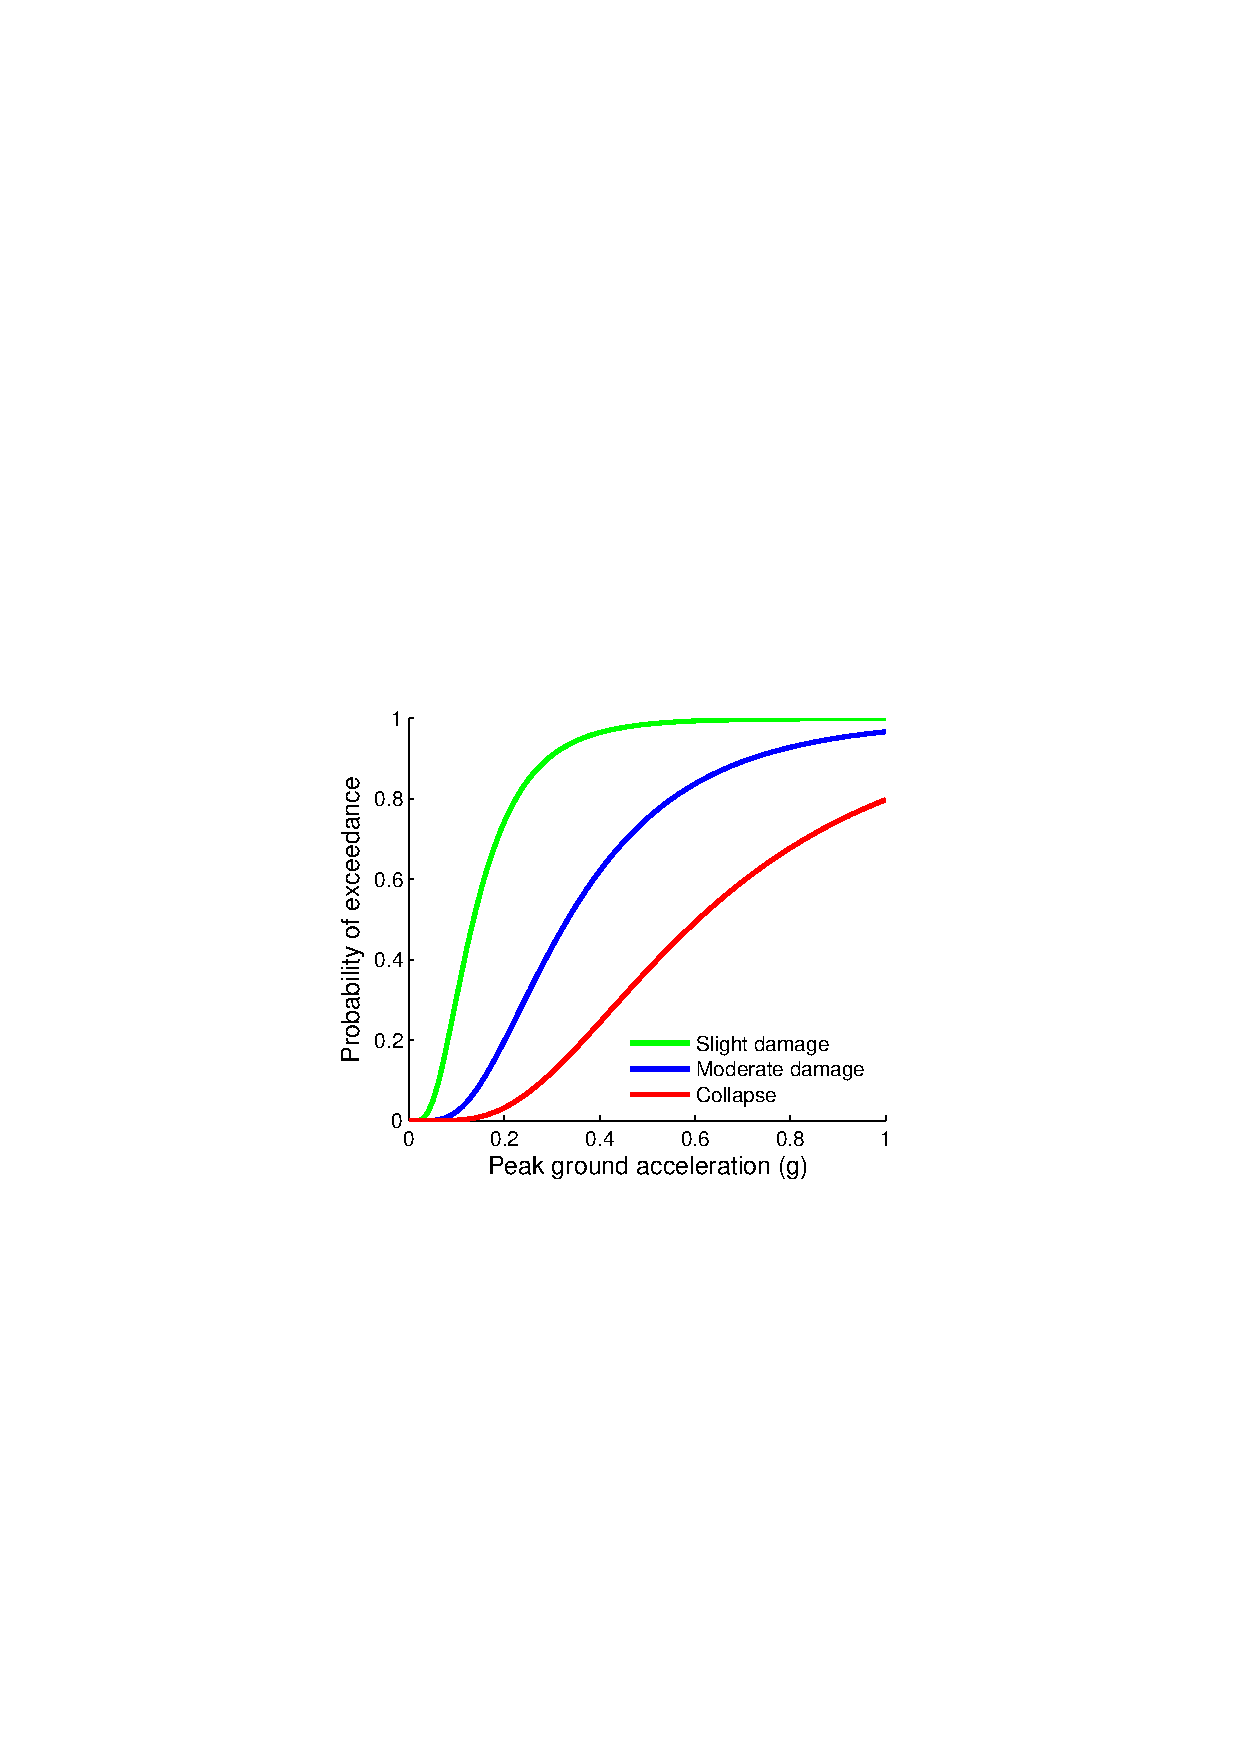
\includegraphics[width=8cm,height=6cm]{figures/risk/ConFragilityModel.pdf}
\caption{Graphical representation of a continuous fragility model.}
\label{fig:fragModelContinuous}
\end{figure}

The NRML schema to store these functions has an initial structure similar to that described for the discrete \glspl{fragility model}. Then, the continuous limit state curves are stored as illustrated below:

\begin{Verbatim}[frame=single, commandchars=\\\{\}, samepage=true]
    ...
    <\textcolor{green}{ffs noDamageLimit= 0.05}>
        <\textcolor{blue}{taxonomy} RC <\textcolor{blue}{/taxonomy}>
        <\textcolor{blue}{IML} IMT="PGA" minIML="0.0" maxIML="1.0" imlUnit="g" ><\textcolor{blue}{/IML}>
        <\textcolor{blue}{ffd} ls="slight">
            <params \textcolor{magenta}{mean}="0.16" \textcolor{magenta}{stddev}="0.11" />
        <\textcolor{blue}{/ffd}
        <\textcolor{blue}{ffd} ls="moderate">
            <params \textcolor{magenta}{mean}="0.40" \textcolor{magenta}{stddev}="0.26" />
        <\textcolor{blue}{/ffd}
        <\textcolor{blue}{ffd} ls="collapse">
            <params \textcolor{magenta}{mean}="0.73" \textcolor{magenta}{stddev}="0.48" />
        <\textcolor{blue}{/ffd}
    <\textcolor{green}{/ffs}>
<\textcolor{red}{/fragilityModel}>
</nrml>
\end{Verbatim}

Again, the set of limit state curves for each building typology needs to be stored within the field \Verb+ffs+ (fragility function set), through the definition of the following attributes:

\begin{itemize}
\item  \Verb+noDamageLimit+: this attribute defines the intensity measure level below which the probability of exceedance for all curves is zero;
\item  \Verb+type+: this parameter defines the type of probabilistic distribution being used to define the limit state curves. Currently the engine only supports lognormal distributions, however, the capability of considering other types of distributions (e.g. normal, exponential) will be developed in the future;
\item  \Verb+taxonomy+: a unique key that is used to relate each \gls{fragility function} with the relevant \glspl{asset} in the \gls{exposure model};
\item  \Verb+IML+: in this field, the intensity measure type (\Verb+IMT+) and associated units (\Verb+imlUnit+) for the limit state curves is defined, along with the minimum (\Verb+minIML+) and maximum (\Verb+maxIML+) intensity measure levels enclosing the range of applicability of the set of fragility functions;
\item  \Verb+ffc+: this field (fragility function continuous) is used to define the mean (\Verb+mean+) and standard deviation (\Verb+stddev+) of the cumulative lognormal function. In addition, the limit state for the curve being defined needs to be specified in the attribute \Verb+ls+.
\end{itemize}

\section{Consequence models}
\label{sec:consequence}
\input{oqum/risk/00c_consequence}

\section{Vulnerability models}
\label{sec:vulnerability}
In this section, the NRML schema for the \gls{vulnerability model} is
described in detail. In order to do so, a graphical representation of a
\gls{vulnerability model} (mean loss ratio for a set of intensity measure
levels) is illustrated in Figure~\ref{fig:vulModel}. Note that although the
uncertainty for each loss ratio is not represented in the aforementioned
figure, it can be considered in the input NRML file, by means of a coefficient
of variation per loss ratio and a probabilistic distribution, which can
currently be set to lognormal (LN) or Beta (BT).

\begin{figure}[ht]
\centering
\includegraphics[width=10cm,height=6cm]{figures/risk/vulnerabilityModel.pdf}
\caption{Graphical representation of a vulnerability model.}
\label{fig:vulModel}
\end{figure}

An example vulnerability model comprising three vulnerability functions is
shown below. This vulnerability model contains one function that uses the 
lognormal distribution to represent the uncertainty in the loss ratio at 
different intensity levels, one function that uses the Beta distribution, and
one function that is defined using a discrete probability mass distribution.

\inputminted[firstline=1,firstnumber=1,fontsize=\footnotesize,frame=single,linenos,bgcolor=lightgray]{xml}{oqum/risk/Verbatim/input_vulnerability.xml}\\


The initial portion of the schema contains general information that describes
some general aspects of the vulnerability model. The information in this
metadata section is common to all of the functions in the vulnerability model
and needs to be included at the beginning of every vulnerability model file.
The parameters are described below:

\begin{itemize}

    \item \Verb+id+: a unique key used to identify the \gls{vulnerability model}

    \item \Verb+assetCategory+: an optional string used to specify the type of
    \glspl{asset} for which vulnerability functions will be defined in this file 
    (e.g: buildings, lifelines)

    \item \Verb+lossCategory+: valid strings for this attribute are 
    ``structural'', ``nonstructural'', ``contents'',  
    ``business\_interruption'', and ``occupants''

    \item \Verb+description+: a brief string with further information about the
    \gls{vulnerability model}, for example, which building typologies are 
    covered or the source of the functions in the \gls{vulnerability model}

\end{itemize}

\inputminted[firstline=4,firstnumber=4,lastline=8,fontsize=\footnotesize,frame=single,linenos,bgcolor=lightgray]{xml}{oqum/risk/Verbatim/input_vulnerability.xml}\\


In order to perform probabilistic or scenario risk calculations, it is
necessary to define a vulnerability function for each building typology
present in the exposure model. The vulnerability functions require the user to
specify the distribution of the loss ratio for a set of intensity levels. The
loss ratio distributions can be defined using either a discrete or a
continuous format, and the fragility model file can include a mix of both
types of vulnerability functions. It is also possible to define a
vulnerability function using a set of deterministic loss ratios corresponding
to a set of intensity levels (i.e., ignoring the uncertainty in the
conditional loss ratios).

The following snippet from the above vulnerability model example file defines
a vulnerability function modelling the uncertainty in the conditional loss
ratios using a (continuous) lognormal distribution:

\inputminted[firstline=10,firstnumber=10,lastline=14,fontsize=\footnotesize,frame=single,linenos,bgcolor=lightgray]{xml}{oqum/risk/Verbatim/input_vulnerability.xml}\\

The following attributes are needed to define a vulnerability function which
uses a continuous distribution to model the uncertainty in the conditional
loss ratios:

\begin{itemize}

    \item \Verb+id+: a unique key used to identify the \gls{taxonomy} for 
    which the function is being defined. This key is used to relate the 
    \gls{vulnerability function} with the relevant \gls{asset} in the 
    \gls{exposure model}.

    \item \Verb+dist+: for vulnerability function which use a continuous 
    distribution to model the uncertainty in the conditional loss ratios, 
    this attribute should be set to either ``\Verb+LN+'' if using the lognormal
    distribution, or to ``\Verb+BT+'' if using the Beta distribution.

    \item \Verb+imls+: this attribute specifies the list of intensity levels
    for which the parameters of the conditional loss ratio distributions will
    be defined. In addition, it is also necessary to define the intensity 
    measure type (\Verb+imt+).

    \item \Verb+meanLRs+: this field is used to define the mean loss ratios
    for this \gls{vulnerability function} for each of the intensity levels
    defined by the attribute \Verb+imls+. The number of mean loss ratios
    defined by the \Verb+meanLRs+ attribute must be equal to the number of
    intensity levels defined by the attribute \Verb+imls+.

    \item \Verb+covLRs+: this field is used to define the coefficient of 
    variation for the conditional distribution of the loss ratios for this
    \gls{vulnerability function} for each of the intensity levels defined by
    the attribute \Verb+imls+. The number of coefficients of variation of loss
    ratios defined by the \Verb+covLRs+ attribute must be equal to the number
    of intensity levels defined by the attribute \Verb+imls+. The uncertainty
    in the conditional loss ratios can be ignored by setting all of the
    \Verb+covLRs+ for a given \gls{vulnerability function} to zero.

\end{itemize}

Several methodologies to derive vulnerability functions are currently being
evaluated by \gls{acr:gem} and have been included as part of the Risk
Modeller's Toolkit, the code for which can be found on a public repository at
GitHub at the following address
\href{http://github.com/gemsciencetools/rmtk}{http://github.com/gemsciencetools/rmtk}.

Scripts to convert \glspl{vulnerability function} in CSV format or as Excel or
ASCII files into NRML are also under development, and can be found at the
OpenQuake platform at the following address:
\href{https://platform.openquake.org/risk_input_preparation_toolkit/}{https://platform.openquake.org/risk\_input\_preparation\_toolkit/}.


\section{Calculation workflows}
\label{sec:risk_workflows}
\subsection{Scenario Damage Assessment}
\index{OpenQuake-engine!Risk calculation workflows!Scenario Damage Assessment}
\label{subsec:workflow_scenario_damage}
This calculator is capable of assessing the damage distribution due to a
single scenario earthquake, for a collection of assets. Similarly to the
previous calculator, in order to perform the necessary risk calculations one
or a set of ground motion fields are required, which can be derived using the
oq-hazardlib, or introduced in the OpenQuake-engine using the appropriate NRML
schema. In this calculator, a fragility model is combined with the
distribution of ground motion at the location of each asset, to estimate the
number or area of buildings in each damage state. The damage distribution can
be extracted per asset, per building typology (taxonomy) or considering all of
the assets simultaneously (total damage distribution). In addition, this
calculator also provides collapse maps, which contain the spatial distribution
of the number or area of collapsed buildings throughout the region of
interest. The input/output structure for this calculator is presented in
Figure~\ref{fig:io-structure-scenario-damage}.

\begin{figure}[ht]
\centering
\includegraphics[width=9cm,height=7cm]{figures/risk/io-structure-scenario-damage.pdf}
\caption{Scenario Damage Calculator input/output structure.}
\label{fig:io-structure-scenario-damage}
\end{figure}

\subsection{Scenario Risk Assessment}
\index{OpenQuake-engine!Risk calculation workflows!Scenario Risk Assessment}
\label{subsec:workflow_scenario_risk}
This calculator computes loss maps and loss statistics due to a single seismic
event, for a collection of assets. The hazard input can be a single ground
motion field (e.g. the median distribution of ground motion in the region of
interest) or a set of ground motion fields allowing the characterisation of
the inter- and intra-event variability from the GMPE. It is noted that the
hazard input can either be calculated using the hazard component of OpenQuake-
engine (oq-hazardlib), or provided to the risk component iian external file
following the respective Natural hazards' Risk Markup Language (NRML) schema
(see \href{http://github.com/gem/oq-nrmllib}{oq-nrmllib}). A vulnerability
model is combined with the distribution of the ground motions at each asset
location to calculate the loss distribution for each asset, as well as the
statistics of the total loss throughout the region of interest. The required
input files and resulting output files are depicted in
Figure~\ref{fig:io-structure-scenario-risk}.

\begin{figure}[ht]
\centering
\includegraphics[width=9cm,height=7cm]{figures/risk/io-structure-scenario-risk.pdf}
\caption{Scenario Risk Calculator input/output structure.}
\label{fig:io-structure-scenario-risk}
\end{figure}

\subsection{Classical Probabilistic Seismic Damage Analysis}
\index{OpenQuake-engine!Risk calculation workflows!Classical Probabilistic Seismic Damage Analysis}
\label{subsec:workflow_classical_damage}
The classical PSHA-based damage calculator convolves through numerical integration, the damage state fragility functions for an asset with the seismic hazard curve at the location of the asset. The main results of this calculator are damage distribution statistics for each asset, which describe the expected fraction of buildings in each damage state. Furthermore, a probabilistic collapse map can be extracted giving the probability of collapse for each asset within the specified time period. Damage distribution aggregated by taxonomy or of the total portfolio (considering all assets in the exposure model) can not be extracted using this calculator, as the spatial correlation of the ground motion residuals is not taken into consideration. The input and output files involved in this calculator are presented in Figure~\ref{fig:ClassicalDamage}.

\begin{figure}[ht]
\centering
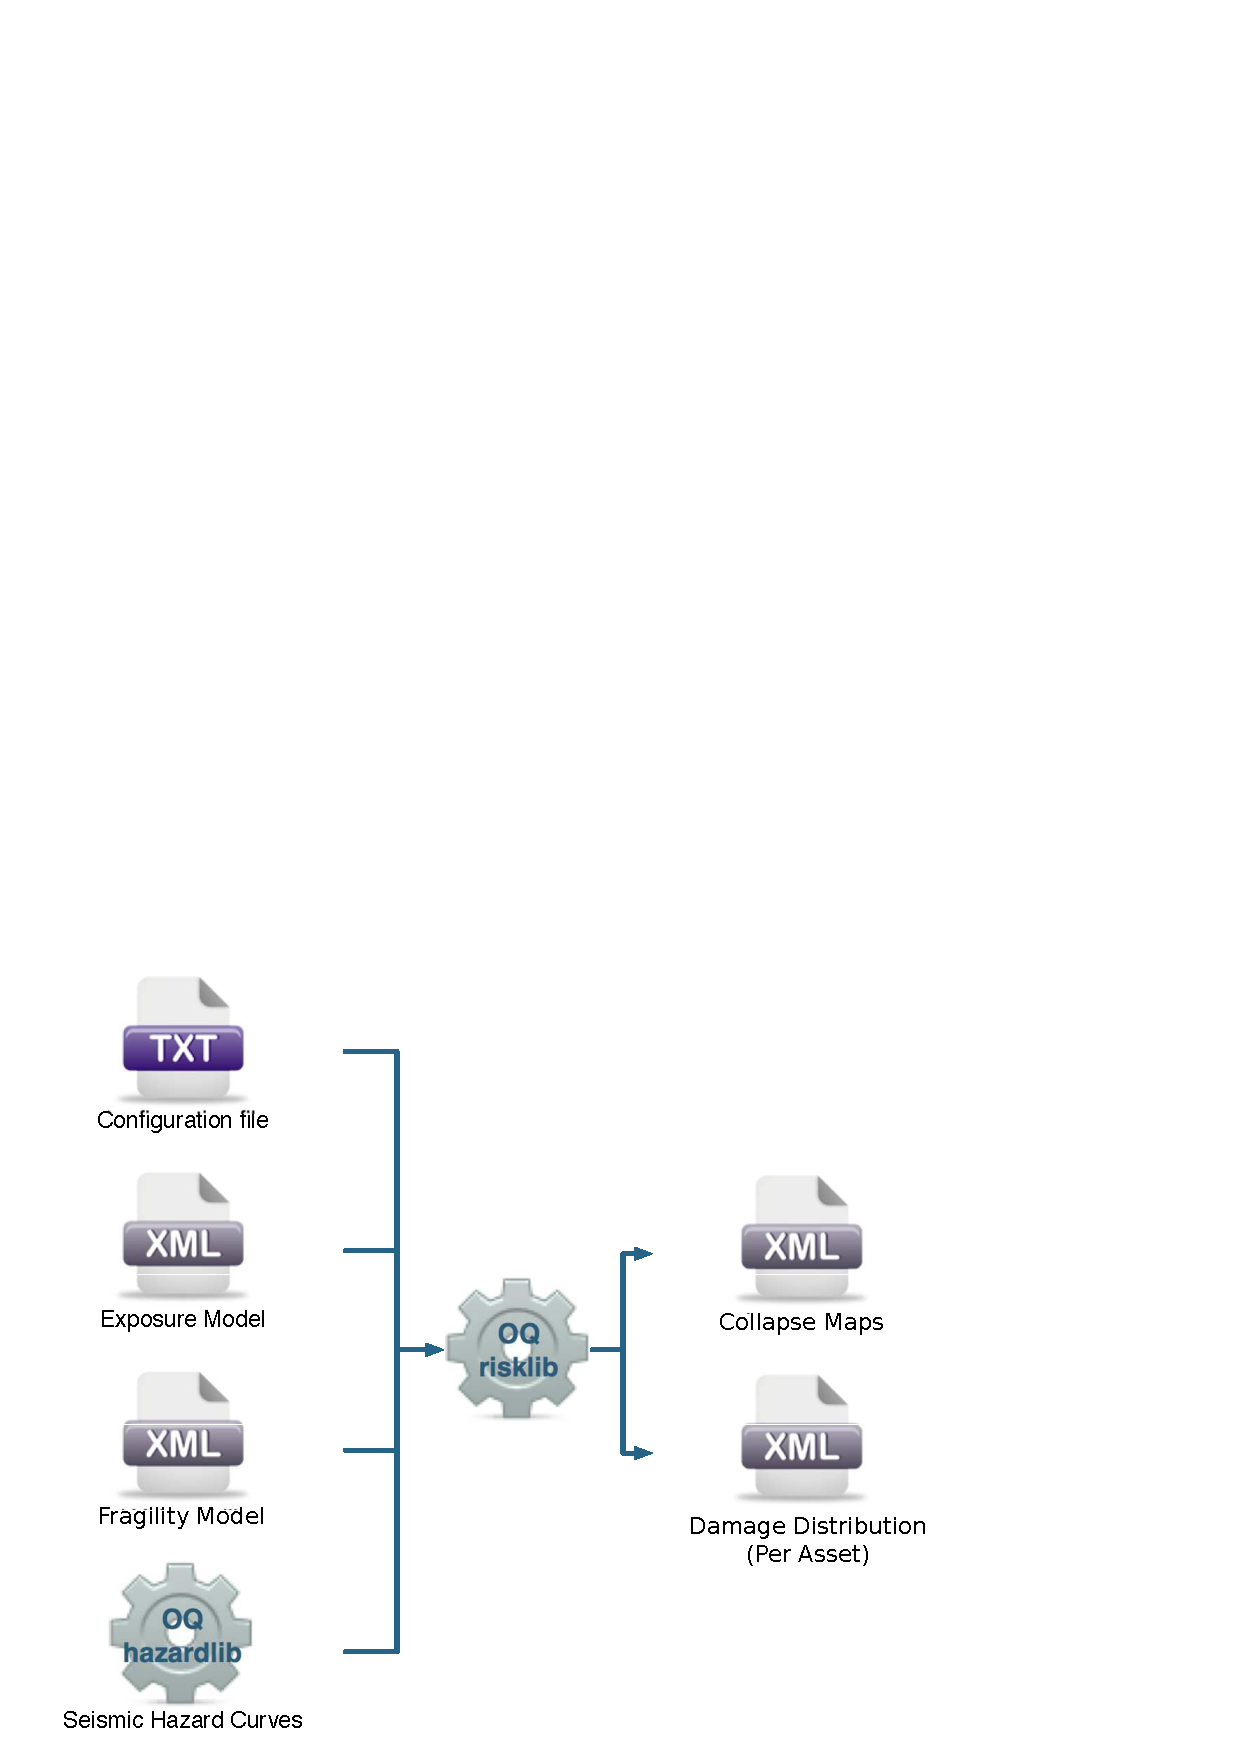
\includegraphics[width=9cm,height=7cm]{figures/risk/ClassicalDamage.pdf}
\caption{Classical PSHA-based Damage Calculator input/output structure.}
\label{fig:ClassicalDamage}
\end{figure}

\subsection{Classical Probabilistic Seismic Risk Analysis}
\index{OpenQuake-engine!Risk calculation workflows!Classical Probabilistic Seismic Risk Analysis}
\label{subsec:workflow_classical_risk}
In this calculator, probabilistic seismic hazard is employed to calculate a loss exceedance curve for each asset, through the usage of seismic hazard curves. A convolution between the vulnerability function and the hazard curve at location of the asset is performed, leading to the probability of exceeding a set of loss ratios. Each loss ratio is multiplied by the asset value to obtain the final loss exceedance curve. Furthermore, probabilistic loss maps can be extracted by interpolating the loss curves at each location by various probabilities of exceedance. Unlike what was described in the previous calculator, a total loss curve (considering all assets in the exposure model) can not be extracted using this calculator, as the correlation of the ground motion residuals and vulnerability uncertainty is not taken into consideration. The input and output files involved in this calculator are presented in Figure~\ref{fig:ClassicalRisk}.

\begin{figure}[ht]
\centering
\includegraphics[width=9cm,height=7cm]{figures/risk/ClassicalRisk.pdf}
\caption{Classical PSHA-based Risk Calculator input/output structure.}
\label{fig:ClassicalRisk}
\end{figure}

\subsection{Event-Based Probabilistic Seismic Risk Analysis}
\index{OpenQuake-engine!Risk calculation workflows!Event-Based Probabilistic Seismic Risk Analysis}
\label{subsec:workflow_event_based_risk}
In this calculator, loss exceedance curves and loss maps for various return
periods can be calculated, based on probabilistic seismic hazard, with an
event-based approach. A large number of stochastic event sets are generated,
and the associated ground motion fields for each event are used together with
a vulnerability model to compute the individual (per asset) and total (sum of
all the losses per event) losses. Then, this distribution of losses is
employed to derive a loss exceedance curve per asset, as well as a total loss
exceedance curve representative of the complete building portfolio.
Furthermore, oq-risklib can also compute loss maps for various return periods
by interpolating each individual loss curve with the respective probability of
exceedance. In Figure~\ref{fig:io-structure-event-based-risk}, the
input/output scheme of this calculator is illustrated.

\begin{figure}[ht]
\centering
\includegraphics[width=9cm,height=7cm]{figures/risk/io-structure-event-based-risk.pdf}
\caption{Probabilistic Event-based Risk Calculator input/output structure.}
\label{fig:io-structure-event-based-risk}
\end{figure}

\subsection{Retrofit Benefit-Cost Ratio Analysis}
\index{OpenQuake-engine!Risk calculation workflows!Retrofit Benefit-Cost Ratio Analysis}
\label{subsec:workflow_benefit_cost}
\input{oqum/risk/00e_workflow_benefit_cost}

\cleardoublepage
   \cleardoublepage

\chapterimage{figures/chapter_head_2.pdf} % Chapter heading image
\chapter{Using the Hazard Module}
	\label{chap:hazinputs}
	This Chapter summarises the structure of the information necessary to define
the different input data to be used with the OpenQuake-engine risk 
calculators.

Input data for scenario-based and probabilistic seismic damage and risk
analysis using OpenQuake-engine are organised into:

\begin{itemize}

  \item A general calculation configuration file.

  \item A file describing the exposure model.

  \item A file describing the vulnerability model for loss calculations, or a 
  		file describing the fragility model for damage calculations. Optionally, 
  		a file describing the consequence model can also be provided in order 
  		to calculate losses from the estimated damage distributions.

  \item Hazard inputs

\end{itemize}

% Figure~\ref{fig:risk_input} summarises the structure of a risk input model
% for the OpenQuake-engine and the relationships between the different files.

% \begin{figure}[!ht]
% \centering
% \includegraphics[width=14cm]{figures/risk/risk_input_structure.pdf}
% \caption{PSHA Input Model structure}
% \label{fig:risk_input}
% \end{figure}

% \section{Defining Logic Trees}
% The main components of a logic tree structure in the OpenQuake engine are 
the following:
\begin{description}
    \item[branch]: the simplest component of a logic tree structure. 
    A branch represent an alternative 
    \item[branching set]: it groups a set of branches i.e. 
    alternative interpretation of a parameter or a model. This set of 
    uncertainties can be applied to the whole initial seismic source input 
    model or to a subset of seismic source data. The sum of the 
    weights/probabilities assigned to the set of branches 
    \item[branching level]: it's the largest container. It's not used in 
    modelling uncertainty, but it's useful in maintaining a logic and an 
    order in the structure of the logic tree as it's will be explained in 
    the following examples.
\end{description}

% \label{sec:risk_logic_trees}

\section{Configuration file}
\index{Input!Configuration file}
\label{sec:risk_configuration_file}
The configuration file (or job.ini file) represents the location where the
paths to the input files, the parameters controlling the risk calculations and
the type of outputs are defined. Some initial parameters common to all the
risk calculators are presented below. The remaining parameters that are
specific to each risk calculator are discussed in subsequent sections. For
additional information about how each parameter is being used within the
methodologies implemented in the oq-engine, users advised to consult the
OpenQuake-engine Book (Risk).

\begin{Verbatim}[frame=single, commandchars=\\\{\}, samepage=true]
[general]
description = Scenario Risk Nepal
calculation_mode = scenario_risk

exposure_file = exposure_model.xml
region_constraint = 78.0 31.5,89.5 31.5,89.5 25.5,78 25.5
asset_hazard_distance = 10
...
\end{Verbatim}

\begin{itemize}
\item  \Verb+description+: a parameter that can be used to include some information about the type of calculations that are going to be performed;
\item  \Verb+calculation_mode+: this parameter sets the type of calculations. The key word for each risk calculator is described in the following sections;
\item  \Verb+exposure_file+: this parameter is used to specify the path to the \gls{exposure model} file;
\item  \Verb+region_constraint+: this field is used to define the polygon enclosing the region of interest. Assets outside of this region will not be considered in the risk calculations. This region is defined using pairs of coordinates (longitude and latitude in decimal degrees) that indicate the vertices of the polygon;
\item  \Verb+asset_hazard_distance+: this parameter indicates the maximum allowable distance between an \gls{asset} and the closest hazard input. If no hazard input is found within this distance, the \gls{asset} is skipped and a message is provided mentioning the id of the asset that is affected by this issue. If this parameter is not provided, the OpenQuake-Engine assumes the maximum allowable distance as 5 km.
\end{itemize}

Depending on the type of calculations, other parameters besides the
aforementioned ones need to be provided, as will be described in the following
sections.

\subsection{Scenario Damage Calculator}
\label{subsec:config_scenario_damage}
For this calculator, the parameter \Verb+calculation_mode+ needs to be defined as \Verb+scenario_damage+. There is only one parameter specific to this calculator, which is the \gls{fragility model} file path, as presented below.

\begin{Verbatim}[frame=single, commandchars=\\\{\}, samepage=true]
...
fragility_file = fragility_model.xml
\end{Verbatim}

\begin{itemize}
\item  \Verb+fragility_file+: a parameter used to define the path to the \gls{fragility model} file.
\end{itemize}

\subsection{Scenario Risk Calculator}
\label{subsec:config_scenario_risk}
In order to run this calculator, the parameter \Verb+calculation_mode+ needs to be set to \Verb+scenario_risk+. The remaining parameters are illustrated bellow.

\begin{Verbatim}[frame=single, commandchars=\\\{\}, samepage=true]
...
structural_vulnerability_file = struct_vul_model.xml
nonstructural_vulnerability_file = nonstruct_vul_model.xml
contents_vulnerability_file = cont_vul_model.xml
business_interruption_vulnerability_file = bus_int_vul_model.xml
occupants_vulnerability_file = occ_vul_model.xml

asset_correlation = 0.7
master_seed = 3
insured_losses = true
\end{Verbatim}

\begin{itemize}
\item  \Verb+structural_vulnerability_file+: this parameter is used to specify the path to the structural \gls{vulnerability model} file;
\item  \Verb+nonstructural_vulnerability_file+: this parameter is used to specify the path to the non-structural\gls{vulnerability model} file;
\item  \Verb+contents_vulnerability_file +: this parameter is used to specify the path to the contents \gls{vulnerability model} file;
\item  \Verb+business_interruption_vulnerability_file +: this parameter is used to specify the path to the business interruption \gls{vulnerability model} file;
\item  \Verb+vulnerability_file+: this parameter is used to specify the path to the occupants \gls{vulnerability model} file;
\item \texttt{asset\_cor\-re\-la\-tion} if the uncertainty in the loss ratios has been defined within the \gls{vulnerability model}, users can specify a coefficient of correlation that will be used in the Monte Carlo sampling process of the loss ratios, between the assets that share the same \gls{taxonomy}. If the \texttt{asset\_cor\-re\-la\-tion} is set to one, the loss ratio residuals will be perfectly correlated. On the other hand, if this parameter is set to zero, the loss ratios will be sampled independently. Any value between zero and one will lead to increasing levels of correlation. If this parameter is not defined, the OpenQuake-engine assumes no correlation in the vulnerability;
\item  \Verb+master_seed+: this parameter is used to control the random generator in the loss ratio sampling process. This way, if the same \Verb+master_seed+ is defined at each calculation run, the same random loss ratios will be generated, thus allowing replicability of the results;
\item  \Verb+insured_losses+: this parameter is used to define if insured losses should be calculated (\Verb+true+) or not (\Verb+false+).
\end{itemize}

\subsection{Classical Probabilistic Seismic Damage Calculator}
\label{subsec:config_classical_damage}
\input{oqum/risk/01a_config_classical_damage}

\subsection{Classical Probabilistic Seismic Risk Calculator}
\label{subsec:config_classical_risk}
\input{oqum/risk/01a_config_classical_risk}

\subsection{Event-Based Probabilistic Seismic Risk Calculator}
\label{subsec:config_event_based_risk}
\input{oqum/risk/01a_config_event_based_risk}

\subsection{Retrofit Benefit-Cost Ratio Calculator}
\label{subsec:config_benefit_cost}
\input{oqum/risk/01a_config_benefit_cost}

\cleardoublepage
   \cleardoublepage

\chapterimage{figures/chapter_head_2.pdf} % Chapter heading image
\chapter{Hazard Calculations and Results}
	\label{chap:hazoutputs}
	In this Chapter we provide a desciption of the main commands available for
running hazard with the \gls{acr:oqe} and the file formats used to represent
the results of the analyses.

A general introduction on the use of the \glsdesc{acr:oqe} is provided in
Section~\ref{sec:running_oq_engine} at page~\pageref{sec:running_oq_engine}. The
reader is invited to consult this part before diving into the following
sections.


% -----------------------------------------------------------------------------
\section{Running OpenQuake-engine for hazard calculations}
\label{sec:running_hazard_calculations}
\index{Running OpenQuake!hazard}

The execution of a hazard analysis using the OpenQuake-engine is
straightforward. Below we provide an example of the simplest command that can be
used to launch a hazard calculation. It consists in the invocation of \texttt
{oq-engine} together with the \texttt{--rh} option which stands for ``run
hazard'' and the name of a configuration file (in the example below it
corresponds to \texttt{job.ini}):

\begin{Verbatim}[frame=single, commandchars=\\\{\}, fontsize=\small]
user@ubuntu:~$ oq-engine --rh job.ini
\end{Verbatim}

The amount of information prompted during the execution of the analysis can be
controlled through the \texttt{--log-level} flag as shown in the example below:

\begin{Verbatim}[frame=single, commandchars=\\\{\}, fontsize=\small]
user@ubuntu:~$ oq-engine --rh job.ini --log-level debug
\end{Verbatim}

In this example we ask the engine to provide an extensive amount of information
(usually not justified for a standard analysis). Alternative options are:
\texttt{debug}, \texttt{info}, \texttt{progress}, \texttt{warn}, \texttt{error},
\texttt{critical}.


% -----------------------------------------------------------------------------
\section{Exporting results from a hazard calculation}
\label{sec:exporting_hazard_results}

There are two alternative ways to get results from the OpenQuake-engine:
directly through the calculation or by exporting them from the internal
\gls{acr:oqe} database once a calculation is completed.

The first option is defined at the OpenQuake-engine invocation through the
flag \texttt{--exports xml}, as shown in the example below:

\begin{Verbatim}[frame=single, commandchars=\\\{\}, fontsize=\small]
user@ubuntu:~$ oq-engine --rh job.ini \textcolor{red}{--exports xml}
\end{Verbatim}

The second option allows the user to export the computed results or just a
subset of them whenever they want. In order to obtain the list of results of
the hazard calculations stored in the \gls{acr:oqe} database the user can
utilize the following command:

\begin{Verbatim}[frame=single, commandchars=\\\{\}, fontsize=\small]
user@ubuntu:~$ oq-engine --lhc
\end{Verbatim}

The execution of this command will produce a list similar to the one provided
below (the numbers in red are the calculations IDs):

\begin{Verbatim}[frame=single, commandchars=\\\{\}, fontsize=\small]
user@ubuntu:~$ oq-engine --lhc
calc_id | num_jobs | latest_job_status | last_update | description
\textcolor{red}{1} | 1 | failed | 2013-03-01 09:49:34 | Classical PSHA
\textcolor{red}{2} | 1 | successful | 2013-03-01 09:49:56 | Classical PSHA
\textcolor{red}{3} | 1 | failed | 2013-03-01 10:24:04 | Classical PSHA
\textcolor{red}{4} | 1 | failed | 2013-03-01 10:28:16 | Classical PSHA
\textcolor{red}{5} | 1 | failed | 2013-03-01 10:30:04 | Classical PSHA
\textcolor{red}{6} | 1 | successful | 2013-03-01 10:31:53 | Classical PSHA
\textcolor{red}{7} | 1 | failed | 2013-03-09 08:15:14 | Classical PSHA
\textcolor{red}{8} | 1 | successful | 2013-03-09 08:18:04 | Classical PSHA
\end{Verbatim}

Subsequently the user can get the list of result stored for a specific hazard
analysis as in the example below (note that the number in blue emphasizes the
result ID):

\begin{Verbatim}[frame=single, commandchars=\\\{\}, fontsize=\small]
user@ubuntu:~$ oq-engine --lho <calc_id>
id | output_type | name
\textcolor{blue}{3} | hazard_curve | hc-rlz-6
\end{Verbatim}

and finally extract an xml file for a specific hazard result:

\begin{Verbatim}[frame=single, commandchars=\\\{\}, fontsize=\small]
user@ubuntu:~$ oq-engine --eh <result_id> <path_to_the_output_folder>
\end{Verbatim}


% -----------------------------------------------------------------------------
\section{Description of hazard outputs}
\label{sec:hazard_outputs}

The results generated by the OpenQuake-engine are fundamentally of two
distinct typologies differentiated by the presence (or absence) of epistemic
uncertainty in the PSHA input model.

When epistemic uncertainty is incorporated into the calculation, the
OpenQuake-engine calculators (e.g. Classical PSHA, Event Based PSHA,
Disaggregation, UHS) produce a set of results (i.e. hazard curves, ground
motion fields, disaggregation matrices, UHS, for each logic-tree realisation)
which reflects epistemic uncertainties introduced in the PSHA input model.

For each logic tree sample, results are computed and stored. Calculation of
results statistics (mean, standard deviation, quantiles) are supported by all
the calculators, with the exception of the disaggregation calculator.

\subsection{Outputs from Classical PSHA}
\label{subsec:output_classical_psha}
By default, the classical PSHA calculator computes and stores hazard curves
for each logic tree sample considered.

When the PSHA input model doesn't contain epistemic uncertainties the results
is a set of hazard curves (one for each investigated site). The command below
illustrates how is possible to retrieve the group of hazard curves obtained
for a calculation with a given identifier \texttt{<calc\_id>} (see
Section~\ref{sec:exporting_hazard_results} for an explanation about how to
obtain the list of calculations performed with their corresponding ID):

\begin{Verbatim}[frame=single, commandchars=\\\{\}, fontsize=\small]
user@ubuntu:~$ oq engine --lo <calc_id>
id | output_type | name
\textcolor{red}{3 | datastore | hcurves}
4  | datastore | realizations
\end{Verbatim}

%The user need not concern them-self with the realizations output. 
%
%In this case the \gls{acr:oqe} computed a group of hazard curves with result
%ID equal to \texttt{3}. On the contrary, if the parameter
%\texttt{number\_of\_logic\_tree\_samples} in the configuration file is
%different than zero, then N hazard curves files are generated. The example
%below shows this case:
%
%\begin{Verbatim}[frame=single, commandchars=\\\{\}, fontsize=\small]
user@ubuntu:~$ oq-engine --lho <calc_id>
id | output_type | name
\textcolor{red}{5 | hazard_curve | hc-rlz-10}
\textcolor{red}{6 | hazard_curve | hc-rlz-7}
\textcolor{red}{7 | hazard_curve | hc-rlz-8}
\textcolor{red}{8 | hazard_curve | hc-rlz-9}
\textcolor{red}{9 | hazard_curve | hc-rlz-11}
\textcolor{red}{10 | hazard_curve | hc-rlz-12}
\end{Verbatim}


To export from the database the outputs (in this case hazard curves)  contained in one of the output identifies, one can do so with the following command:

\begin{Verbatim}[frame=single, commandchars=\\\{\}, fontsize=\small]
user@ubuntu:~$ oq engine --export-output <output_id> <output_directory>
\end{Verbatim}

Alternatively, if the user wishes to export all of the outputs associated with a particular calculation then they can use the \texttt{-{}-export-outputs} with the corresponding calculation key:

\begin{Verbatim}[frame=single, commandchars=\\\{\}, fontsize=\small]
user@ubuntu:~$ oq engine --export-outputs <calc_id> <output_directory>
\end{Verbatim}

The exports will produce one or more nrml files containing the seismic hazard curves, as represented in the example in the inset
below:

\input{oqum/hazard/verbatim/output_hazard_curves}

Notwithstanding the intuitiveness of this file, let's have a brief
overview of the information included.

The overall content of this file is a list of hazard curves, one for each
investigated site, computed using a PSHA input model representing one possible
realisation obtained using the complete logic tree structure.

The attributes of the \texttt{hazardCurves} element (see text in red) specify
the path of the logic tree used to create the seismic source model
(\texttt{source\-Model\-TreePath}) and the ground motion model
(\texttt{gsim\-Tree\-Path}) plus the intensity measure type and the
investigation time used to compute the probability of exceedance.

The \texttt{IMLs} element (in green in the example) contains the values of
shaking used by the engine to compute the probability of exceedance in the
investigation time. For each site this file contains a \texttt{hazardCurve}
element which has the coordinates (longitude and latitude in decimal degrees)
of the site and the values of the probability of exceedance for all the
intensity measure levels specified in the \texttt{IMLs} element.

If the hazard calculation is configured to produce results including seismic hazard maps and uniform hazard spectra, then the list of outputs would display the following:

\begin{Verbatim}[frame=single, commandchars=\\\{\}, fontsize=\small]
user@ubuntu:~$ oq engine --lo <calc_id>
id | output_type | name
\textcolor{red}{3 | datastore | hcurves}
\textcolor{red}{4 | datastore | hmaps}
5  | datastore | realizations
\textcolor{red}{6 | datastore | uhs}
\end{Verbatim}

%\input{oqum/hazard/verbatim/output_classical_multiple_rlz}

%In this example the \gls{acr:oqe} produced hazard curves and hazard maps for
%six logic tree realisations plus median hazard curves and the median hazard
%map (both highlighted in red).

The following inset shows a sample of the nrml file used to describe a hazard map:

\input{oqum/hazard/verbatim/output_hazard_map}

\noindent and a uniform hazard spectrum:

\input{oqum/hazard/verbatim/output_uhs}

\subsection{Outputs from Hazard Disaggregation}
\label{subsec:output_hazard_disaggregation}
\section{Output from Disaggregation}
The \gls{acr:oqe} output of a disaggregation analysis  
corresponds to the combination of a hazard curve and a multidimensional 
matrix containing the results of the disaggregation.

The example below shows the list of disaggregation results obtained 
for four logic tree realisations. 
%
For each realisation, disaggregation has been completed for two  
intensity measure levels corresponding to different probabilities of 
exceedence in the specified \texttt{investigation time}.
\begin{Verbatim}[frame=single, commandchars=\\\{\}]
user@ubuntu:~$ openquake --lho <calc_id> 
id | output_type | name
19 | hazard_curve | hc-rlz-3
20 | hazard_curve | hc-rlz-3
21 | hazard_curve | hc-rlz-4
22 | hazard_curve | hc-rlz-4
23 | disagg_matrix | disagg(0.02)-rlz-3-SA(0.025)-POINT(10.1 40.1)
24 | disagg_matrix | disagg(0.1)-rlz-3-SA(0.025)-POINT(10.1 40.1)
25 | disagg_matrix | disagg(0.02)-rlz-3-PGA-POINT(10.1 40.1)
26 | disagg_matrix | disagg(0.1)-rlz-3-PGA-POINT(10.1 40.1)
27 | disagg_matrix | disagg(0.02)-rlz-4-SA(0.025)-POINT(10.1 40.1)
28 | disagg_matrix | disagg(0.1)-rlz-4-SA(0.025)-POINT(10.1 40.1)
29 | disagg_matrix | disagg(0.02)-rlz-4-PGA-POINT(10.1 40.1)
30 | disagg_matrix | disagg(0.1)-rlz-4-PGA-POINT(10.1 40.1)
\end{Verbatim}

In the following inset we show an example of the nrml file 
used to represent the different disaggregation matrices (highlighted 
in red) produced by OpenQuake-engine.
%
\begin{Verbatim}[frame=single, commandchars=\\\{\}, fontsize=\small]
<?xml version='2.0' encoding='UTF-8'?>
<nrml xmlns:gml="http://www.opengis.net/gml" 
      xmlns="http://openquake.org/xmlns/nrml/0.4">
  <disaggMatrices sourceModelTreePath="b1" gsimTreePath="b1" IMT="PGA" 
        investigationTime="50.0" lon="10.1" lat="40.1" 
        magBinEdges="5.0, 6.0, 7.0, 8.0" 
        distBinEdges="0.0, 25.0, 50.0, 75.0, 100.0" 
        lonBinEdges="9.0, 10.5, 12.0" 
        latBinEdges="39.0, 40.5" 
        epsBinEdges="-3.0, -1.0, 1.0, 3.0" 
        tectonicRegionTypes="Active Shallow Crust">
\textcolor{red}{    <disaggMatrix type="Mag" dims="3" poE="0.1" }
\textcolor{red}{            iml="0.033424622602">}
      <prob index="0" value="0.987374744394"/>
      <prob index="1" value="0.704295394366"/>
      <prob index="2" value="0.0802318409498"/>
\textcolor{red}{    </disaggMatrix>}
\textcolor{red}{    <disaggMatrix type="Dist" dims="4" poE="0.1" }
\textcolor{red}{            iml="0.033424622602">}
      <prob index="0" value="0.700851969171"/>
      <prob index="1" value="0.936680387051"/>
      <prob index="2" value="0.761883595568"/>
      <prob index="3" value="0.238687565571"/>
\textcolor{red}{    </disaggMatrix>}
\textcolor{red}{    <disaggMatrix type="TRT" dims="1" poE="0.1" }
\textcolor{red}{            iml="0.033424622602">}
      <prob index="0" value="0.996566187011"/>
\textcolor{red}{    </disaggMatrix>}
\textcolor{red}{    <disaggMatrix type="Mag,Dist" dims="3,4" poE="0.1" }
\textcolor{red}{            iml="0.033424622602">}
      <prob index="2,3" value="0.0"/>
\textcolor{red}{    </disaggMatrix>}
\textcolor{red}{    <disaggMatrix type="Mag,Dist,Eps" dims="3,4,3" poE="0.1" }
\textcolor{red}{            iml="0.033424622602">}
      <prob index="0,0,0" value="0.0785857271425"/>
      ...
\textcolor{red}{    </disaggMatrix>}
\textcolor{red}{    <disaggMatrix type="Lon,Lat" dims="2,1" poE="0.1"}
\textcolor{red}{            iml="0.033424622602">}
      <prob index="0,0" value="0.996566187011"/>
      <prob index="1,0" value="0.0"/>
\textcolor{red}{    </disaggMatrix>}
\textcolor{red}{    <disaggMatrix type="Mag,Lon,Lat" dims="3,2,1" poE="0.1"} 
\textcolor{red}{            iml="0.033424622602">}
      <prob index="0,0,0" value="0.987374744394"/>
      <prob index="0,1,0" value="0.0"/>
      <prob index="1,0,0" value="0.704295394366"/>
      <prob index="1,1,0" value="0.0"/>
      <prob index="2,0,0" value="0.0802318409498"/>
      <prob index="2,1,0" value="0.0"/>
\textcolor{red}{    </disaggMatrix>}
\textcolor{red}{    <disaggMatrix type="Lon,Lat,TRT" dims="2,1,1" poE="0.1"} 
\textcolor{red}{            iml="0.033424622602">}
      <prob index="0,0,0" value="0.996566187011"/>
      <prob index="1,0,0" value="0.0"/>
\textcolor{red}{    </disaggMatrix>}
  </disaggMatrices>
</nrml>

\end{Verbatim}
%\caption{Hazard map: nrml sample file}
%\label{vrb:disaggr}
%\end{nrmlsmp}



\subsection{Outputs from Event Based PSHA}
\label{subsec:output_event_based_psha}
The Event Based PSHA calculator computes and stores stochastic event sets and
the corresponding ground motion fields.

This calculator can also produce hazard curves and hazard maps exactly in the
same way as done using the Classical PSHA calculator.

The inset below shows an example of the list of results provided by the
\gls{acr:oqe} at the end of an event-based PSHA calculation:

\begin{Verbatim}[frame=single, commandchars=\\\{\}, fontsize=\small]
user@ubuntu:~$ oq-engine --lho <calc_id>
id | output_type | name
\textcolor{red}{31 | ses | ses-coll-rlz-19}
\textcolor{green}{32 | gmf | gmf-rlz-19}
\textcolor{red}{33 | ses | ses-coll-rlz-20}
\textcolor{green}{34 | gmf | gmf-rlz-20}
35 | hazard_curve | hazard-curve-rlz-19-SA(0.1)
36 | hazard_curve | hazard-curve-rlz-20-SA(0.1)
37 | hazard_curve | hazard-curve-rlz-19-PGA
38 | hazard_curve | hazard-curve-rlz-20-PGA
39 | hazard_curve | mean curve for SA(0.1)
40 | hazard_curve | quantile curve (poe >= 0.15) for imt SA(0.1)
41 | hazard_curve | quantile curve (poe >= 0.50) for imt SA(0.1)
42 | hazard_curve | quantile curve (poe >= 0.85) for imt SA(0.1)
43 | hazard_curve | mean curve for PGA
44 | hazard_curve | quantile curve (poe >= 0.15) for imt PGA
45 | hazard_curve | quantile curve (poe >= 0.50) for imt PGA
46 | hazard_curve | quantile curve (poe >= 0.85) for imt PGA
\end{Verbatim}

This list in the inset above contains two sets of stochastic events (in red)
and two sets of ground motion fields (in blue).

The whole group of stochastic event set and ground motion fields can be
exported immediately using the results with \texttt{id} 35 and 25, respectively.

Below is an example showing a nrml file containing a collection of stochastic
event sets (2 ruptures):

\input{oqum/hazard/verbatim/output_ses}

The text in red shows the part which describes the id of the generated
stochastic event set and the investigation time covered.

The text in green emphasises the portion of the text used to describe a
rupture. The information provided describes entirely the geometry of the rupture as well as its rupturing properties (e.g. rake, magnitude). The rupture ID is a string that represents each rupture uniquely (including the case where the same rupture is sampled multiple times). The exact format may be subject to change from time-to-time; however, the ID will usually contain information regarding the specific logic tree branch sample (realisation), the stochastic event set counter, the ID of the source from which the rupture was samples and a unique number indicating the rupture identifier within the earthquake rupture forecast of the specific source.

This is an example of a nrml file containing one ground motion field:

\input{oqum/hazard/verbatim/output_gmf}


   \cleardoublepage

\chapterimage{figures/chapter_head_2.pdf} % Chapter heading image
\chapter{Demonstrative Examples}
	\label{chap:hazdemos}
	% -----------------------------------------------------------------------------
\section{OpenQuake Hazard Demos}
With the \gls{acr:oqe} installation a number of demos are provided showing practical examples
of input and configuration files definition for different use cases.
The following demos illustrate how to use \gls{acr:oqe} for various seismic hazard analysis:
\begin{itemize}
\item PointSourceClassicalPSHA
\item AreaSourceClassicalPSHA
\item SimpleFaultSourceClassicalPSHA
\item ComplexFaultSourceClassicalPSHA
\item CharacteristicFaultSourceCase1ClassicalPSHA
\item CharacteristicFaultSourceCase2ClassicalPSHA
\item CharacteristicFaultSourceCase3ClassicalPSHA
\item LogicTreeCase1ClassicalPSHA
\item LogicTreeCase2ClassicalPSHA
\item LogicTreeCase3ClassicalPSHA
\item EventBasedPSHA
\item Disaggregation
\end{itemize}

\subsection{Classical PSHA Demos}
A number of demos have been designed to show how to perform a classical PSHA calculation using the different available
source typologies and how to define non-trivial logic trees. It should be noted that the input files that will be illustrated are valid
not only for a classical PSHA calculation but also for event based and disaggregation analysis.\\

\subsubsection{Classical PSHA with different source typologies}
All the classical PSHA demos illustrating the different source typologies (all demos but the ones about Logic Tree definition)
share the following GSIM logic tree file:
\begin{Verbatim}[frame=single, commandchars=\\\{\}, fontsize=\normalsize]
<?xml version="1.0" encoding="UTF-8"?>

<nrml xmlns:gml="http://www.opengis.net/gml"
      xmlns="http://openquake.org/xmlns/nrml/0.4">
    <logicTree logicTreeID='lt1'>

        <logicTreeBranchingLevel branchingLevelID="bl1">
            <logicTreeBranchSet
               uncertaintyType="gmpeModel"
               applyToTectonicRegionType="Active Shallow Crust"
               branchSetID="bs1">

                <logicTreeBranch branchID="b1">
                     <uncertaintyModel>
                        BooreAtkinson2008
                     </uncertaintyModel>
                     <uncertaintyWeight>1.0</uncertaintyWeight>
                </logicTreeBranch>

            </logicTreeBranchSet>
        </logicTreeBranchingLevel>

    </logicTree>
</nrml>
\end{Verbatim}
Each source in the source model file is defined as belonging to \texttt{Active Shallow Crust}, and therefore the GSIM Logic Tree file
defines for simplicity a single GMPE (Boore and Atkinson 2008) which is associated to an \texttt{Active Shallow Crust} tectonic region type.\\
The configuration file is defined to compute hazard curves for several intensity measure types (PGV, PGA and Spectral
acceleration at different periods), hazard maps and uniform hazard spectra for different probabilities of exceedance:
\begin{Verbatim}[frame=single, commandchars=\\\{\}, fontsize=\normalsize]
[general]

description = ...
calculation_mode = classical
random_seed = 23

[geometry]

region = ...
region_grid_spacing = 5.0

[logic_tree]

number_of_logic_tree_samples = 0

[erf]

rupture_mesh_spacing = 2
width_of_mfd_bin = 0.1
area_source_discretization = 5.0

[site_params]

reference_vs30_type = measured
reference_vs30_value = 600.0
reference_depth_to_2pt5km_per_sec = 5.0
reference_depth_to_1pt0km_per_sec = 100.0

[calculation]

source_model_logic_tree_file = source_model_logic_tree.xml
gsim_logic_tree_file = gmpe_logic_tree.xml
investigation_time = 50.0
intensity_measure_types_and_levels =\{
"PGV": [2, 4, 6 ,8, 10, ...], 
"PGA": [0.005, 0.007, ...], 
"SA(0.025)": [...], 
"SA(0.05)": [...],
"SA(0.1)": [...], 
"SA(0.2)": [...], 
"SA(0.5)": [...], 
"SA(1.0)": [...],
"SA(2.0)": [...]\}
truncation_level = 3
maximum_distance = 200.0

[output]

export_dir = ...
mean_hazard_curves = false
quantile_hazard_curves =
hazard_maps = true
uniform_hazard_spectra = true
poes = 0.1 0.02
\end{Verbatim}
Hazard maps for the different demos are show in figure \ref{fig:hazard_maps1} and \ref{fig:hazard_maps2}.

\begin{figure} 
\centering 
\subcaptionbox{}
{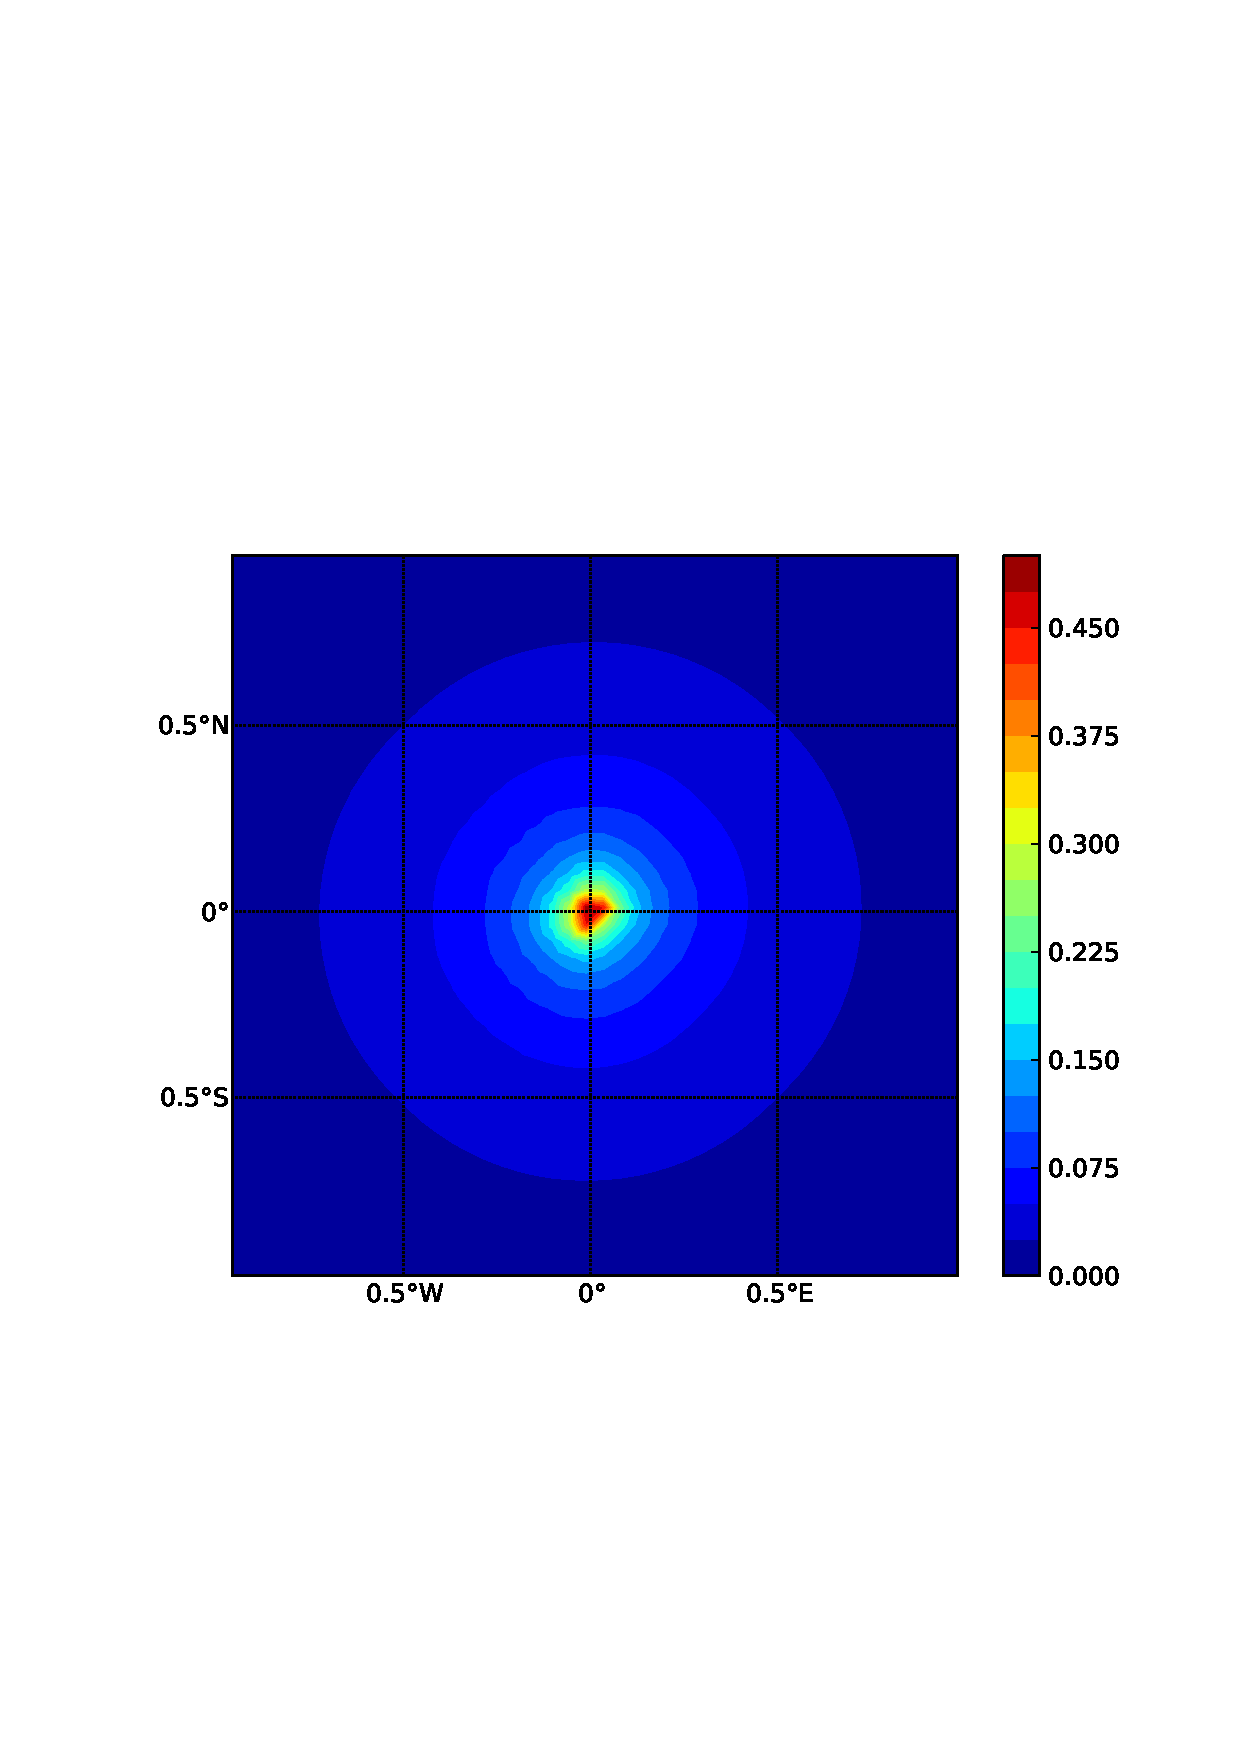
\includegraphics[width=7cm]{./figures/hazard/point.pdf}} 
\subcaptionbox{}
{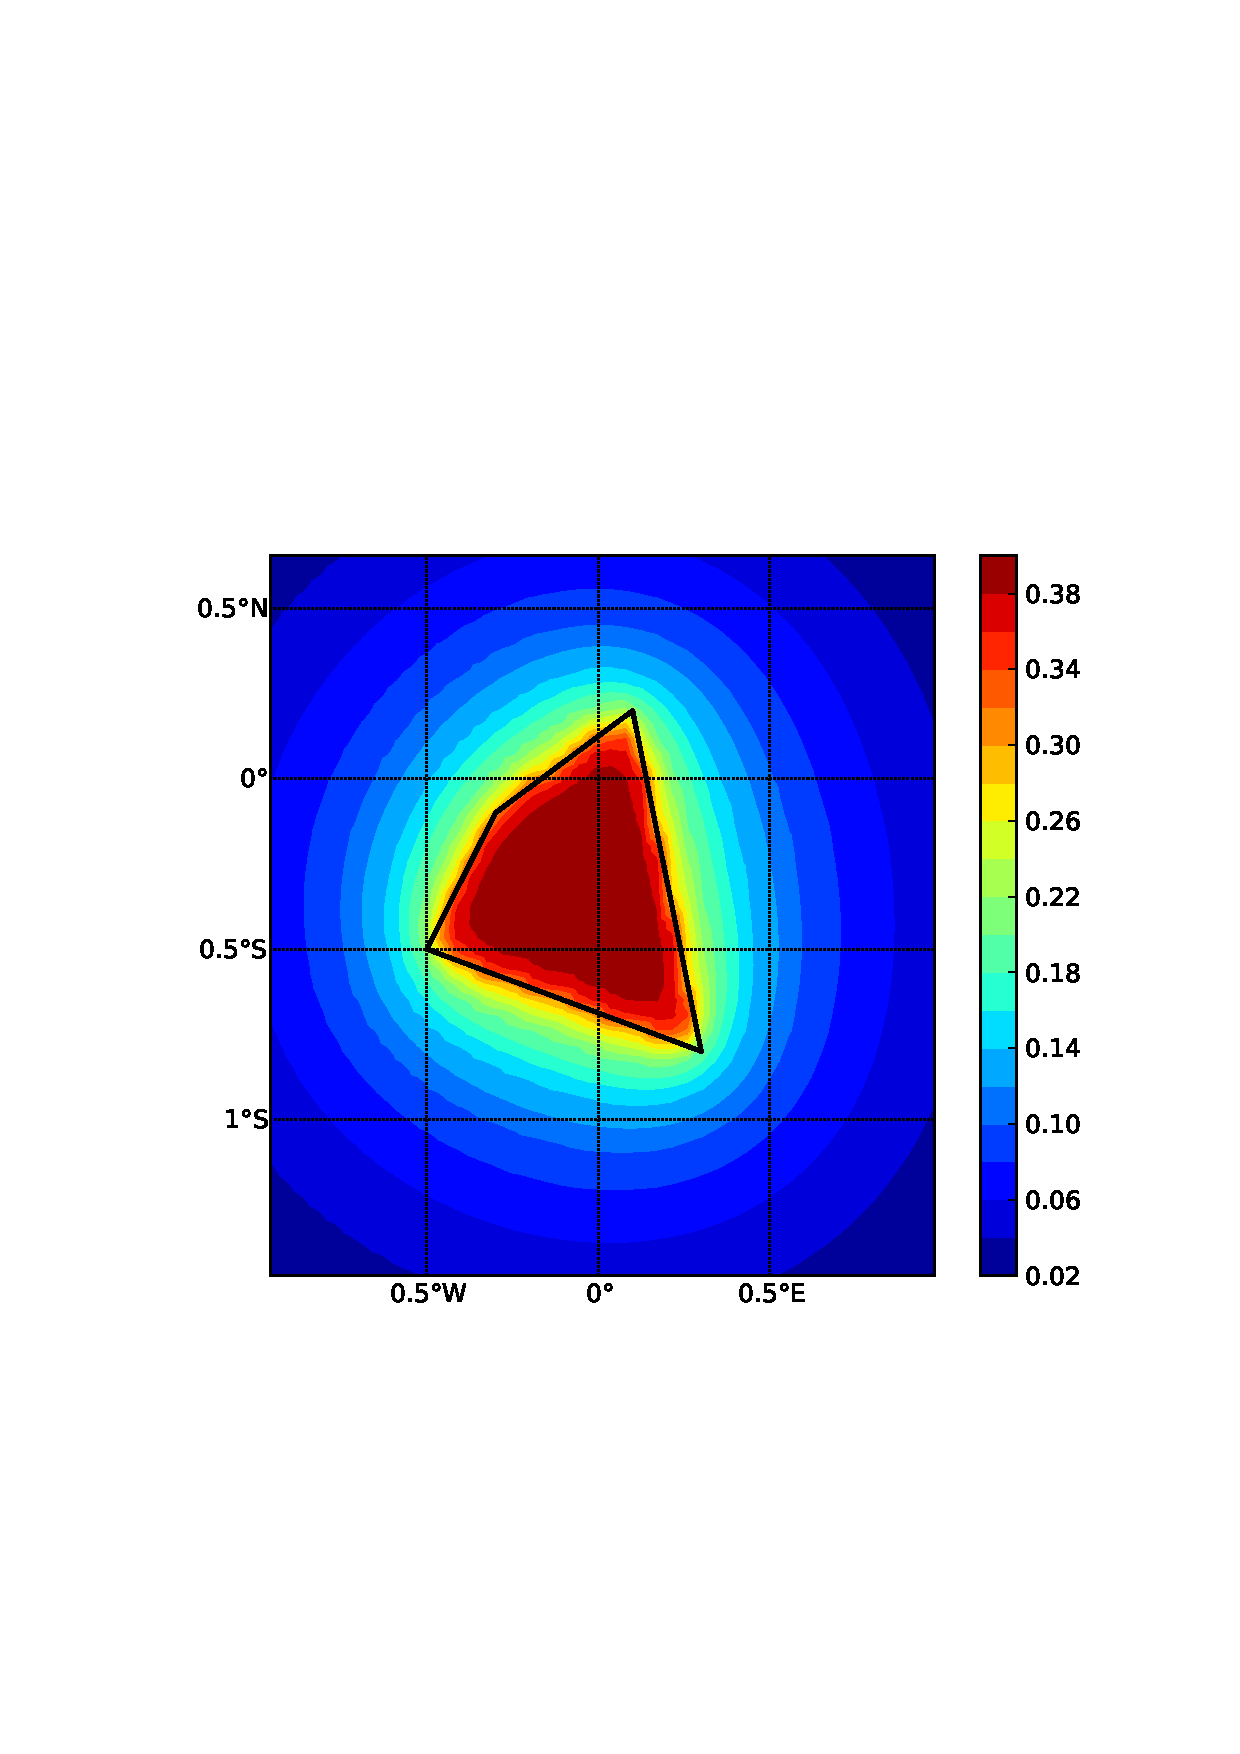
\includegraphics[width=7cm]{./figures/hazard/area.pdf}} 
\subcaptionbox{}
{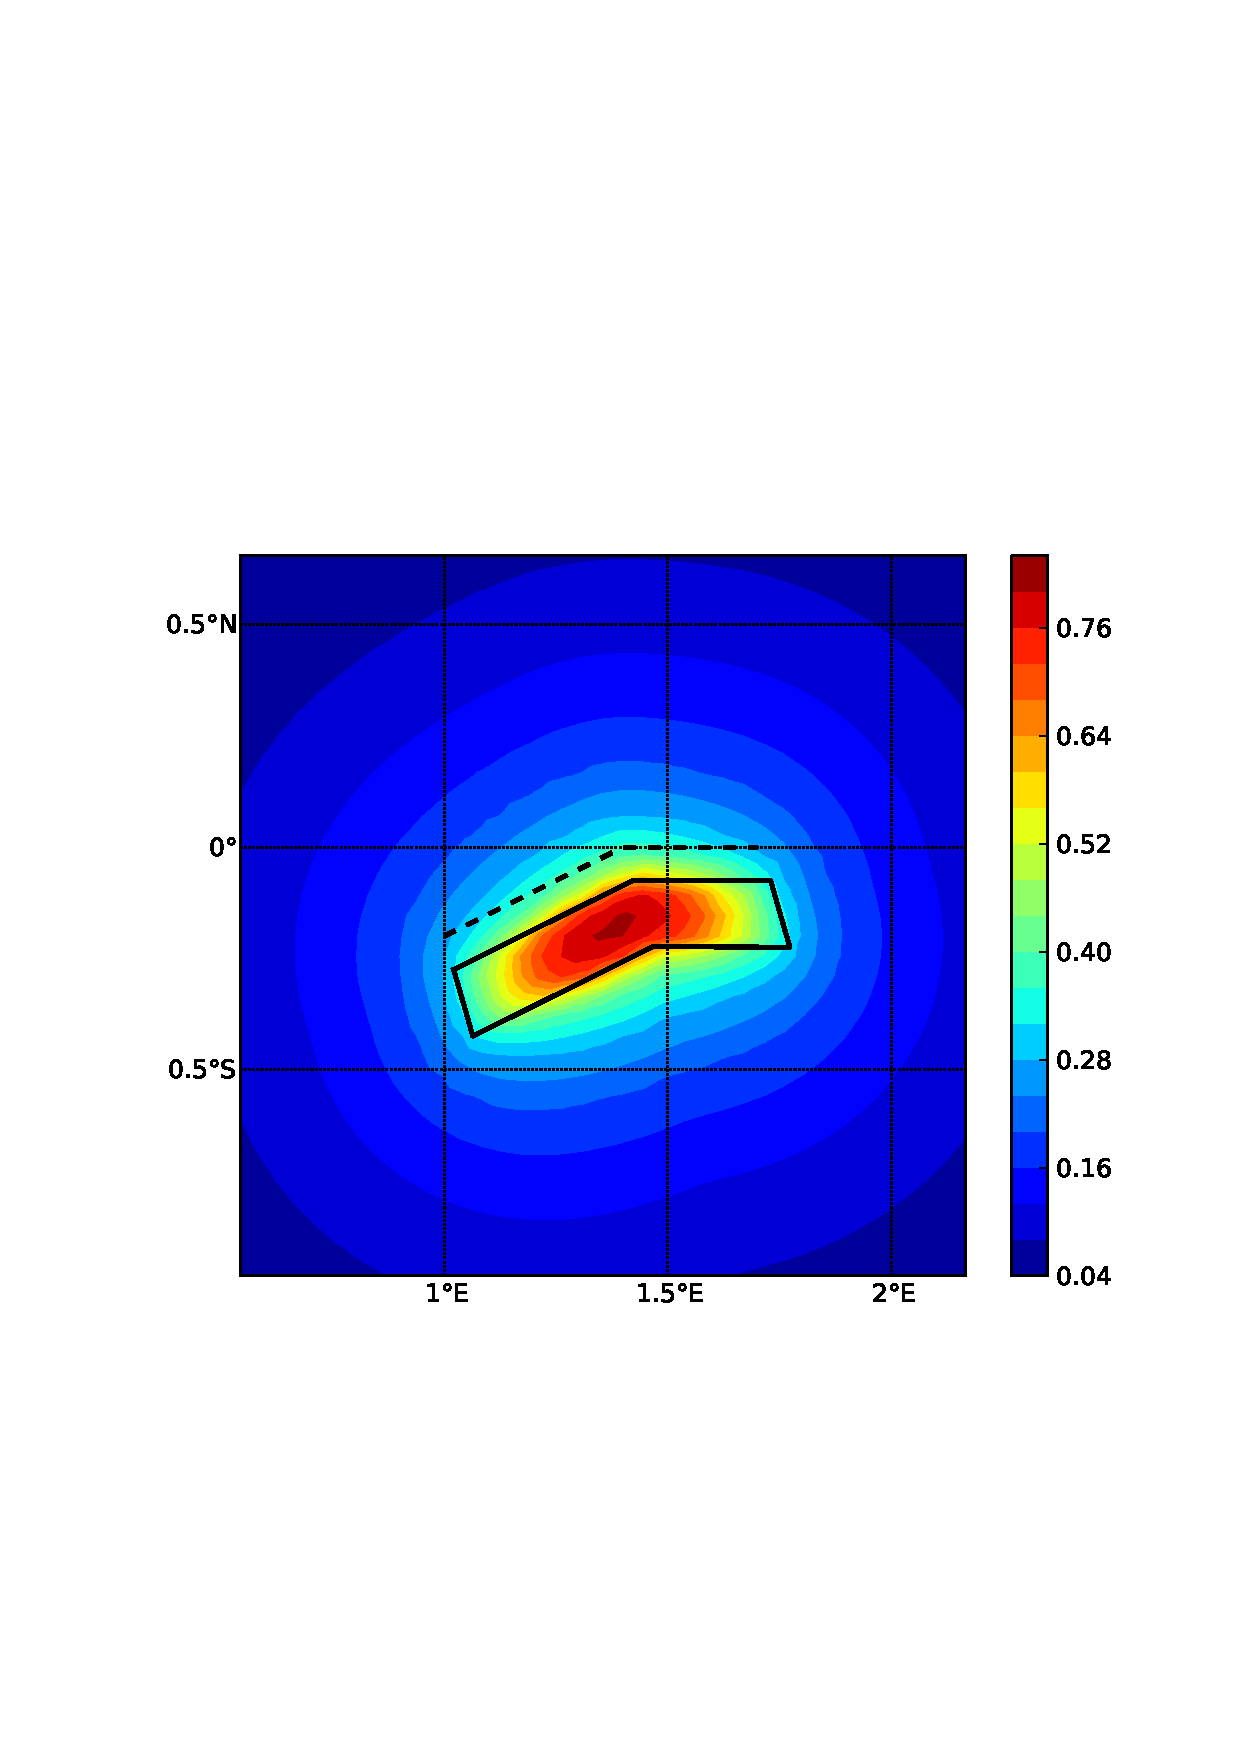
\includegraphics[width=7cm]{./figures/hazard/simple_fault.pdf}} 
\subcaptionbox{}
{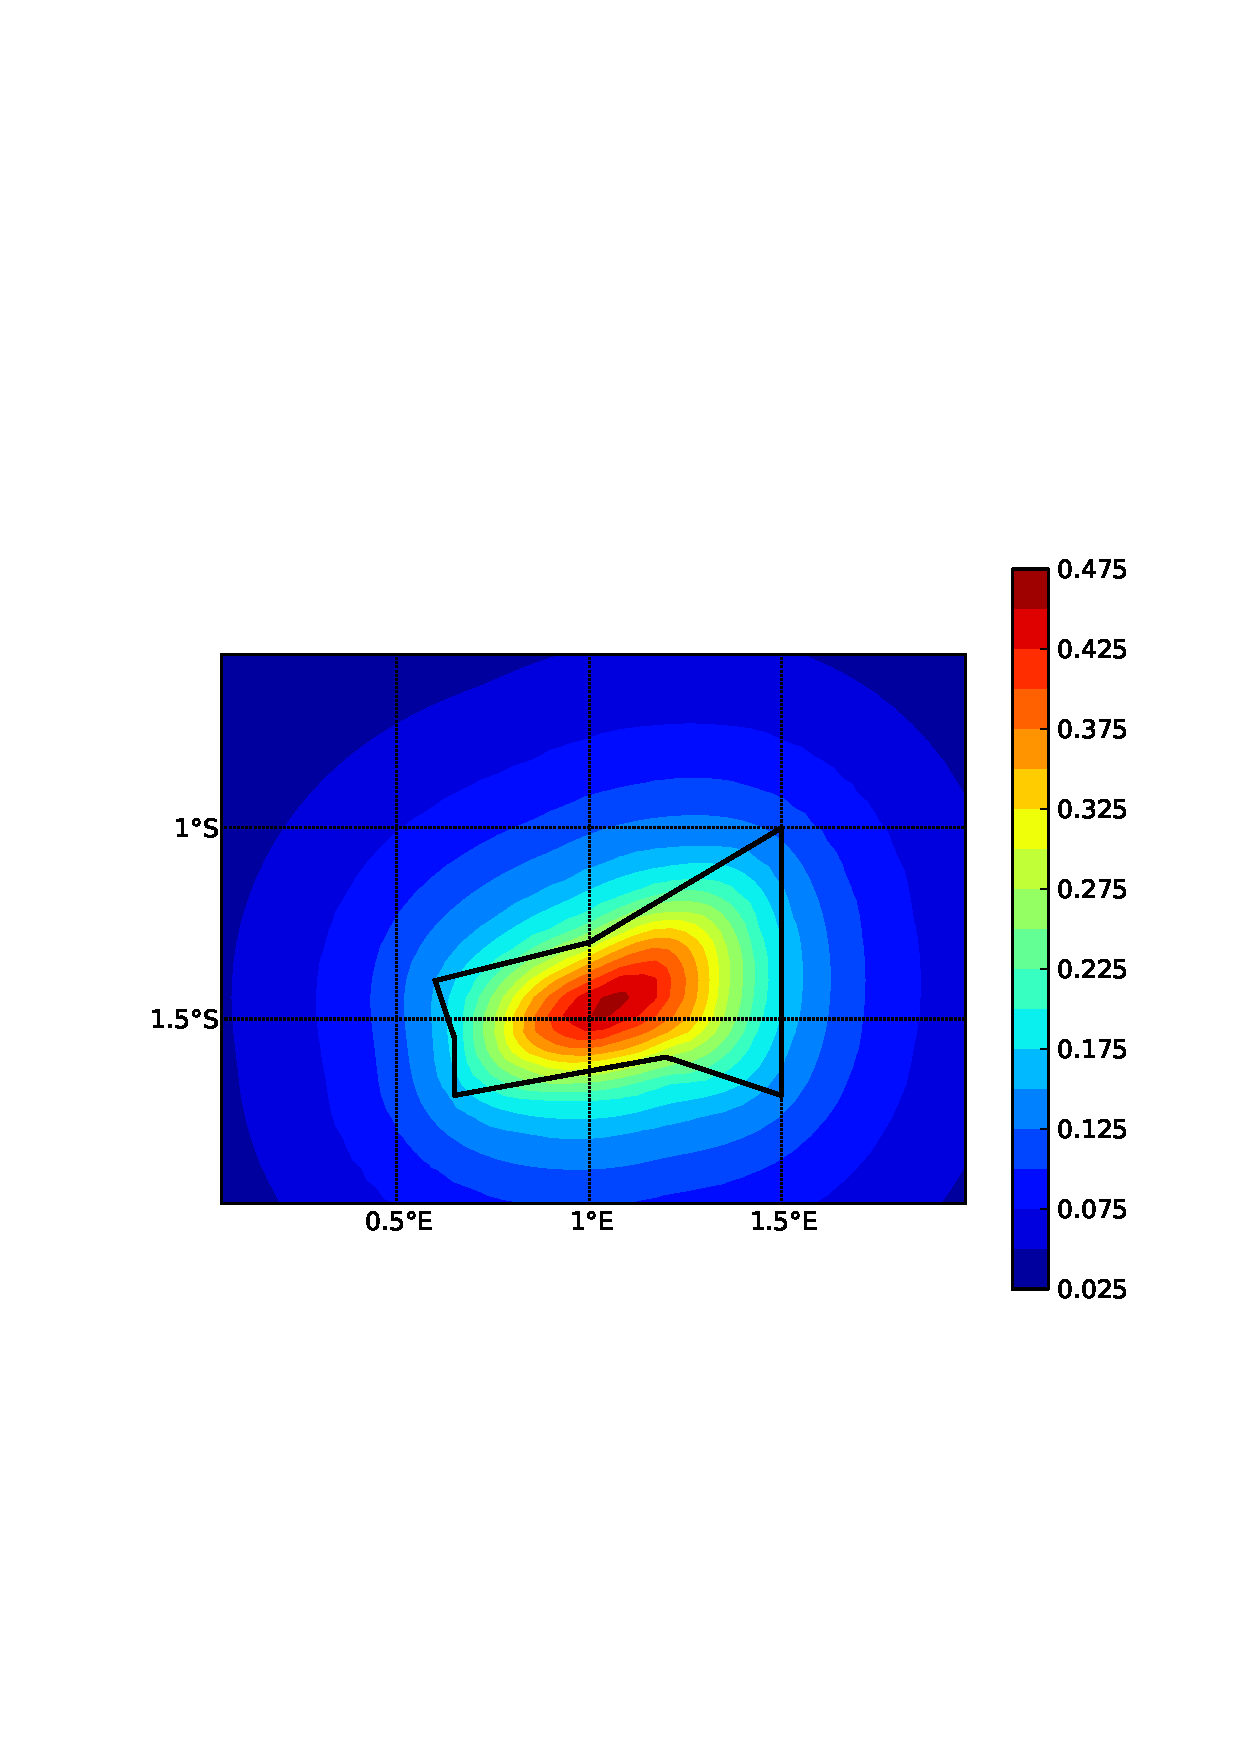
\includegraphics[width=7cm]{./figures/hazard/complex_fault.pdf}} 
\caption{Hazard maps (for PGA, 10\% in 50 years) as obtained from the different \gls{acr:oqe} source typologies. (a) Point Source. (b) Area source. 
The solid black line represents the area boundary. (c) Simple Fault Source. The dashed line represents the fault trace, while the solid line the fault
surface projection. (d) Complex Fault Source. The solid line represent the fault surface projection (d)}
\label{fig:hazard_maps1}
\end{figure}

\begin{figure} 
\centering 
\subcaptionbox{}
{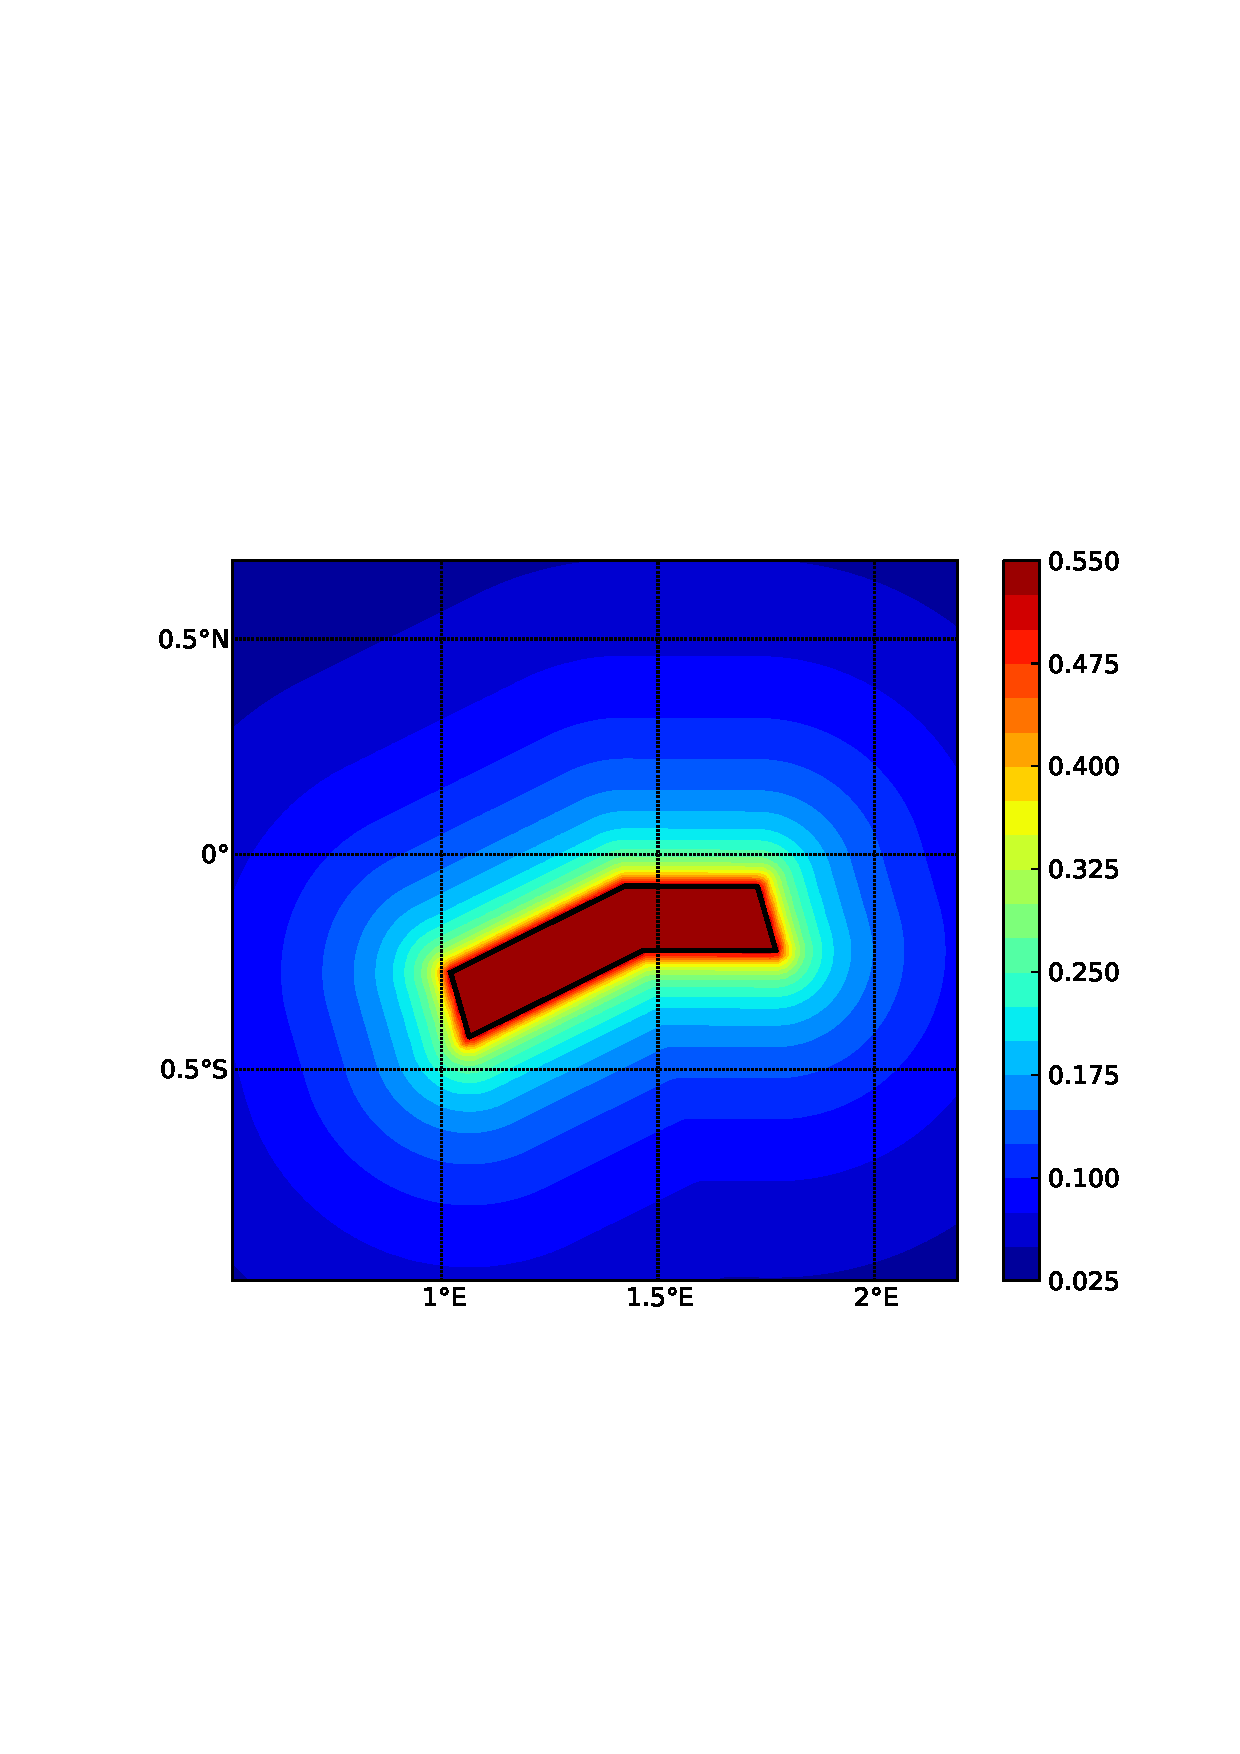
\includegraphics[width=7cm]{./figures/hazard/char_fault2.pdf}} 
\subcaptionbox{}
{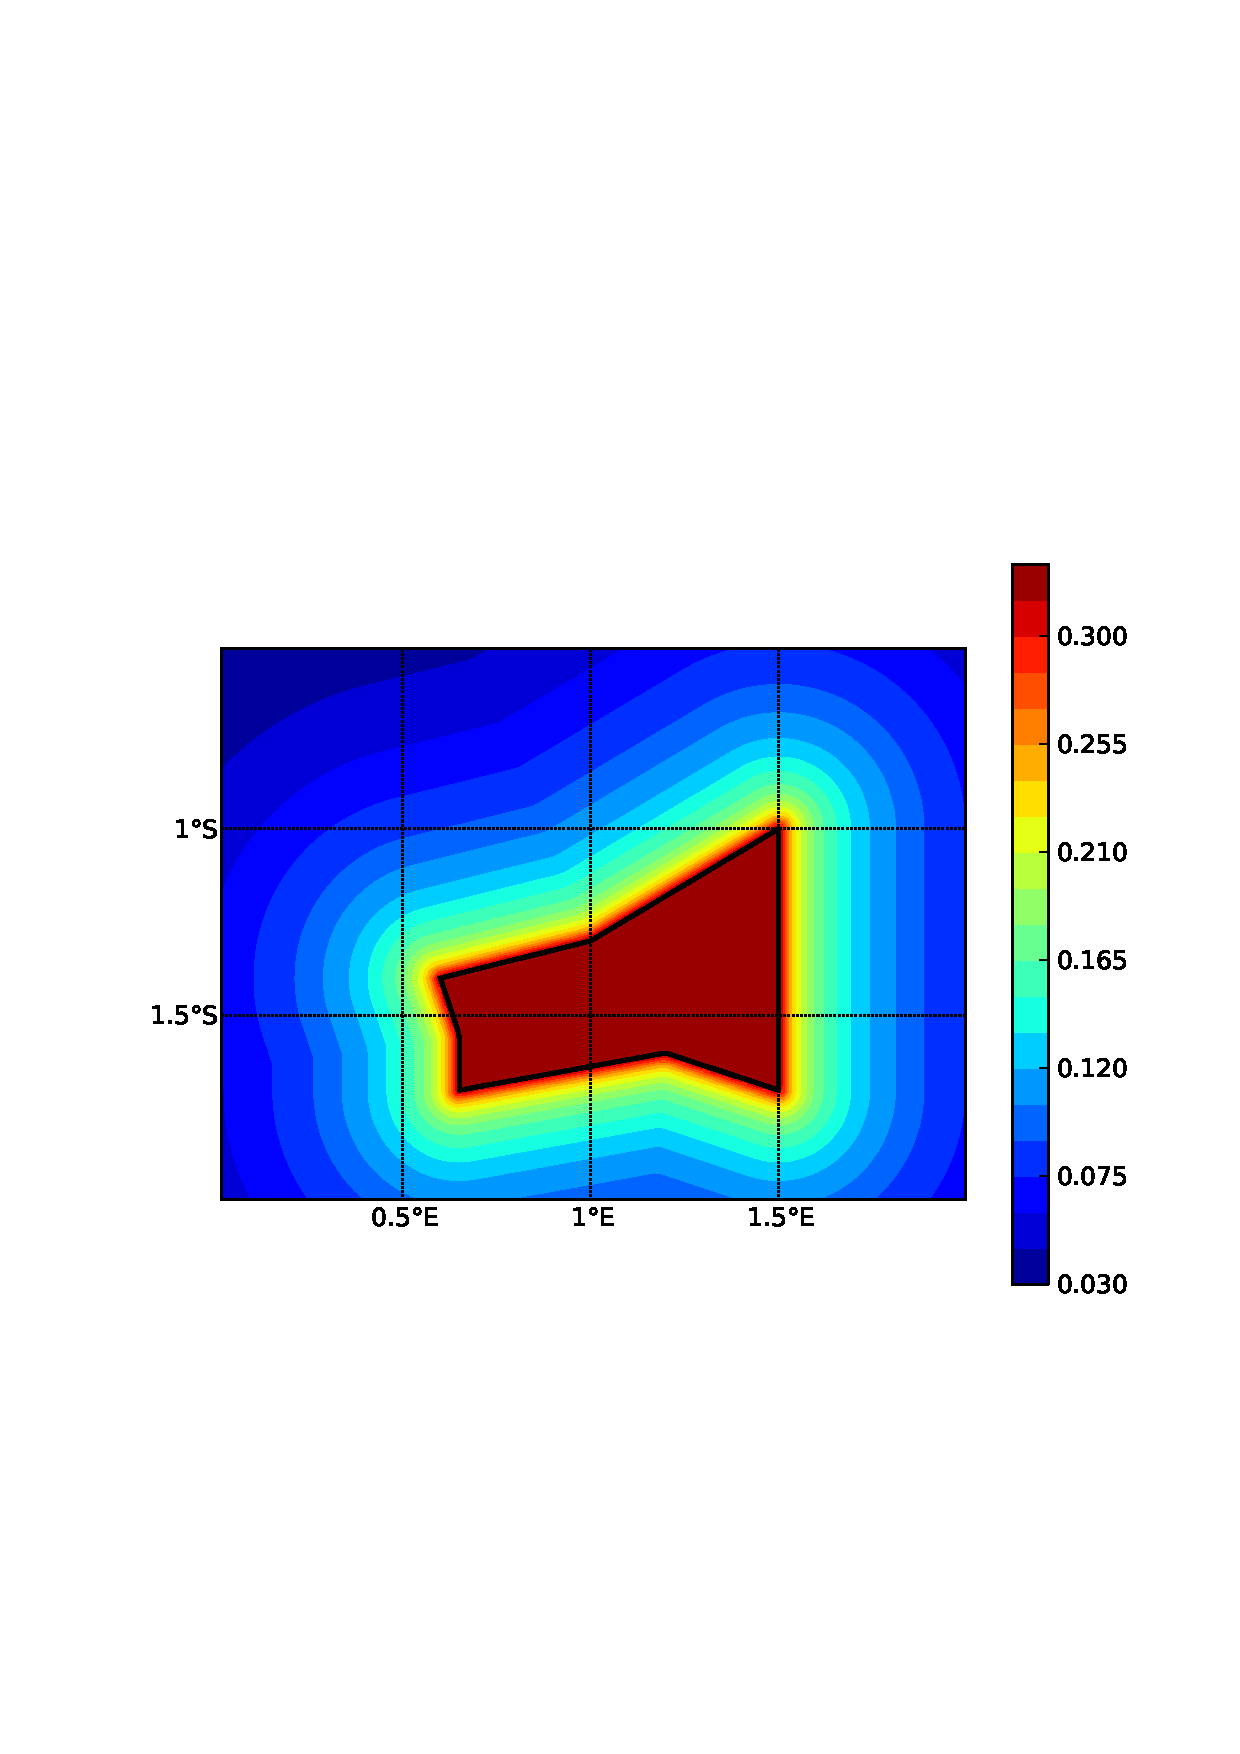
\includegraphics[width=7cm]{./figures/hazard/char_fault3.pdf}} 
\subcaptionbox{}
{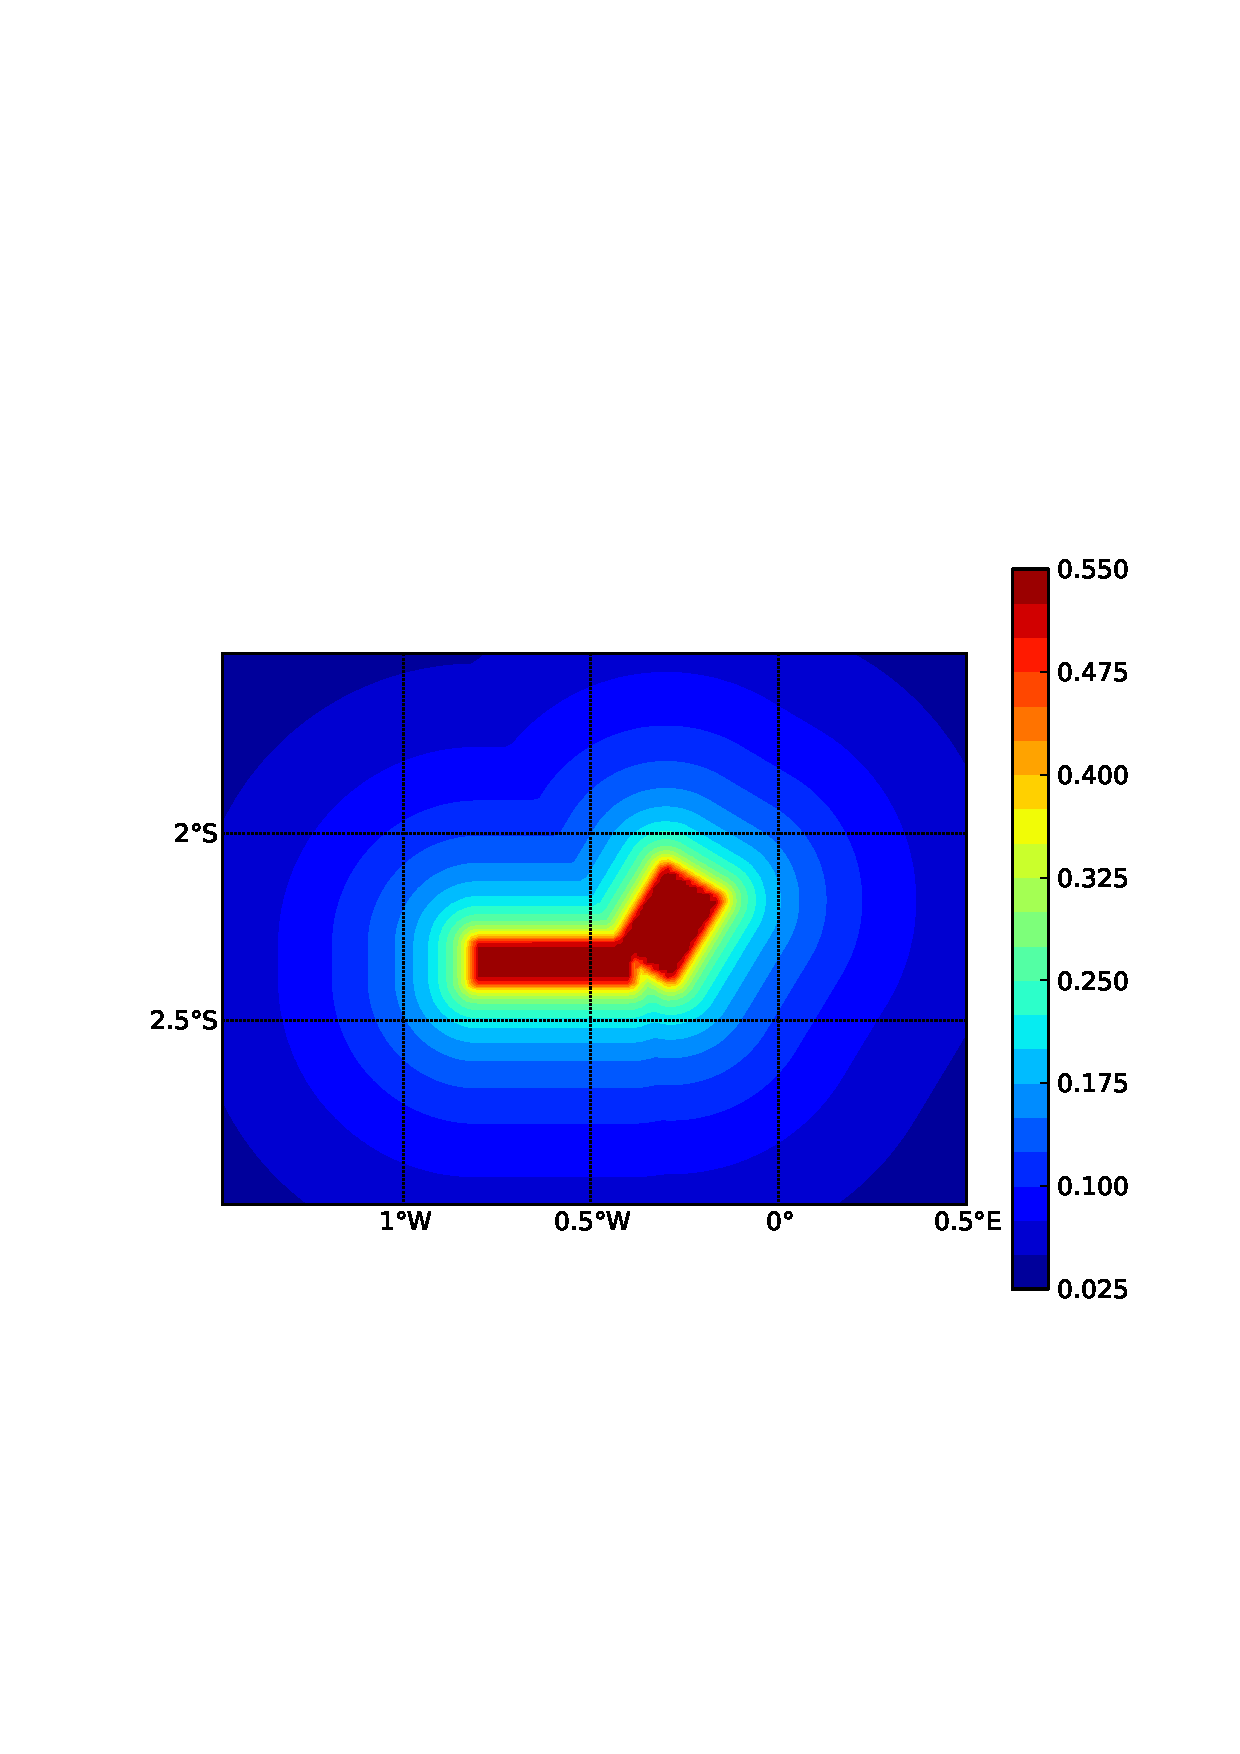
\includegraphics[width=7cm]{./figures/hazard/char_fault1.pdf}} 
\caption{Hazard maps (for PGA, 10\% in 50 years) as obtained from characteristic fault sources with simple fault
geometry (e), complex fault geometry (f), and collection of planar surfaces (g)}
\label{fig:hazard_maps2}
\end{figure}


\subsubsection{Classical PSHA with non trivial logic trees}
Three demos are provided to illustrate how the logic tree formalism can be used to express epistemic uncertainties in seismic hazard analysis.\\

LogicTreeCase1ClassicalPSHA shows an example of logic tree defining two alternative source models, with sources belonging to two different
tectonic region types, and with two alternative GMPEs for each tectonic region type.
The source model logic tree is therefore defined in the following way:
\begin{Verbatim}[frame=single, commandchars=\\\{\}, fontsize=\normalsize]
<?xml version="1.0" encoding="UTF-8"?>
<nrml xmlns:gml="http://www.opengis.net/gml"
      xmlns="http://openquake.org/xmlns/nrml/0.4">
    <logicTree logicTreeID="lt1">

        <logicTreeBranchingLevel branchingLevelID="bl1">

            <logicTreeBranchSet uncertaintyType="sourceModel"
                                branchSetID="bs1">
                <logicTreeBranch branchID="b1">
                    <uncertaintyModel>
                      source_model_1.xml
                    </uncertaintyModel>
                    <uncertaintyWeight>0.5</uncertaintyWeight>
                </logicTreeBranch>
                <logicTreeBranch branchID="b2">
                    <uncertaintyModel>
                       source_model_2.xml
                    </uncertaintyModel>
                    <uncertaintyWeight>0.5</uncertaintyWeight>
                </logicTreeBranch>
            </logicTreeBranchSet>

        </logicTreeBranchingLevel>

    </logicTree>
</nrml>
\end{Verbatim}
The two source models are defined in two different source model files \texttt{source\_\-model\_\-1.xml} and \texttt{source\_\-model\_\-2.xml} each
associated to the corresponding weight (0.5 in both cases).\\
The GSIM logic tree file contains the following structure:
\begin{Verbatim}[frame=single, commandchars=\\\{\}, fontsize=\normalsize]
<?xml version="1.0" encoding="UTF-8"?>

<nrml xmlns:gml="http://www.opengis.net/gml"
      xmlns="http://openquake.org/xmlns/nrml/0.4">
    <logicTree logicTreeID='lt1'>

        <logicTreeBranchingLevel branchingLevelID="bl1">
            <logicTreeBranchSet uncertaintyType="gmpeModel"
               applyToTectonicRegionType="Active Shallow Crust"
               branchSetID="bs1">
                <logicTreeBranch branchID="b11">
                   <uncertaintyModel>
                      BooreAtkinson2008
                   </uncertaintyModel>
                   <uncertaintyWeight>0.5</uncertaintyWeight>
                </logicTreeBranch>
                <logicTreeBranch branchID="b12">
                   <uncertaintyModel>
                      ChiouYoungs2008
                   </uncertaintyModel>
                   <uncertaintyWeight>0.5</uncertaintyWeight>
                </logicTreeBranch>
            </logicTreeBranchSet>
        </logicTreeBranchingLevel>

        <logicTreeBranchingLevel branchingLevelID="bl2">
            <logicTreeBranchSet uncertaintyType="gmpeModel"
              applyToTectonicRegionType="Stable Continental Crust"
              branchSetID="bs2">
              <logicTreeBranch branchID="b21">
                <uncertaintyModel>
                   ToroEtAl2002</uncertaintyModel>
                <uncertaintyWeight>0.5</uncertaintyWeight>
                </logicTreeBranch>
                <logicTreeBranch branchID="b22">
                  <uncertaintyModel>
                     Campbell2003</uncertaintyModel>
                  <uncertaintyWeight>0.5</uncertaintyWeight>
                </logicTreeBranch>
            </logicTreeBranchSet>
        </logicTreeBranchingLevel>

    </logicTree>
</nrml>
\end{Verbatim}
The source model contains sources belonging to Active Shallow Crust and Stable Continental Crust, therefore the
GSIM logic tree defines two branching levels, one for each considered tectonic region type. Moreover for each tectonic
region type a branch set with two GMPEs is defined: Boore and Atkinson 2008 and Chiou and Youngs 2008 for Active
Shallow Crust and Toro et al. 2003 and Campbell 2003 for Stable Continental Crust. By processing the above logic tree
files using the logic tree path enumeration mode (enabled by setting in the configuration file \texttt{number\_\-of\_\-logic\_\-tree\_\-samples = 0})
hazard results are obtained for 8 logic tree paths (2 source models x 2 GMPEs for Active x 2 GMPEs for Stable).\\

LogicTreeCase2ClassicalPSHA defines a single source model consisting of only two sources (area and simple fault) belonging to different
tectonic region types (Active Shallow Crust and Stable Continental Region) and both characterized by a truncated Gutenberg-Richter distribution.
The logic tree defines uncertainties for G-R a, b values (three possible pairs for each source) and maximum magnitude (three values for each source) 
and uncertainties on the GMPEs for each tectonic region type (two GMPE per region type).\\
To accomodate such a structure the GSIM logic tree is defined in the following way:
\begin{Verbatim}[frame=single, commandchars=\\\{\}, fontsize=\normalsize]
<?xml version="1.0" encoding="UTF-8"?>
<nrml xmlns:gml="http://www.opengis.net/gml"
      xmlns="http://openquake.org/xmlns/nrml/0.4">
    <logicTree logicTreeID="lt1">

        <logicTreeBranchingLevel branchingLevelID="bl1">
            <logicTreeBranchSet uncertaintyType="sourceModel"
                                branchSetID="bs1">
                <logicTreeBranch branchID="b11">
                    <uncertaintyModel>
                     source_model.xml
                    </uncertaintyModel>
                    <uncertaintyWeight>1.0</uncertaintyWeight>
                </logicTreeBranch>
            </logicTreeBranchSet>
        </logicTreeBranchingLevel>

        <logicTreeBranchingLevel branchingLevelID="bl2">
            <logicTreeBranchSet uncertaintyType="abGRAbsolute"
                                applyToSources="1"
                                branchSetID="bs21">
                <logicTreeBranch branchID="b21">
                    <uncertaintyModel>4.6 1.1</uncertaintyModel>
                    <uncertaintyWeight>0.333</uncertaintyWeight>
                </logicTreeBranch>
                <logicTreeBranch branchID="b22">
                    <uncertaintyModel>4.5 1.0</uncertaintyModel>
                    <uncertaintyWeight>0.333</uncertaintyWeight>
                </logicTreeBranch>
                <logicTreeBranch branchID="b23">
                    <uncertaintyModel>4.4 0.9</uncertaintyModel>
                    <uncertaintyWeight>0.334</uncertaintyWeight>
                </logicTreeBranch>
            </logicTreeBranchSet>
        </logicTreeBranchingLevel>

        <logicTreeBranchingLevel branchingLevelID="bl3">
            <logicTreeBranchSet uncertaintyType="abGRAbsolute"
                                applyToSources="2"
                                branchSetID="bs31">
                <logicTreeBranch branchID="b31">
                    <uncertaintyModel>3.3 1.0</uncertaintyModel>
                    <uncertaintyWeight>0.333</uncertaintyWeight>
                </logicTreeBranch>
                <logicTreeBranch branchID="b32">
                    <uncertaintyModel>3.2 0.9</uncertaintyModel>
                    <uncertaintyWeight>0.333</uncertaintyWeight>
                </logicTreeBranch>
                <logicTreeBranch branchID="b33">
                    <uncertaintyModel>3.1 0.8</uncertaintyModel>
                    <uncertaintyWeight>0.334</uncertaintyWeight>
                </logicTreeBranch>
            </logicTreeBranchSet>
        </logicTreeBranchingLevel>

        <logicTreeBranchingLevel branchingLevelID="bl4">
            <logicTreeBranchSet uncertaintyType="maxMagGRAbsolute"
                                applyToSources="1"
                                branchSetID="bs41">
                <logicTreeBranch branchID="b41">
                    <uncertaintyModel>7.0</uncertaintyModel>
                    <uncertaintyWeight>0.333</uncertaintyWeight>
                </logicTreeBranch>
                <logicTreeBranch branchID="b42">
                    <uncertaintyModel>7.3</uncertaintyModel>
                    <uncertaintyWeight>0.333</uncertaintyWeight>
                </logicTreeBranch>
                <logicTreeBranch branchID="b43">
                    <uncertaintyModel>7.6</uncertaintyModel>
                    <uncertaintyWeight>0.334</uncertaintyWeight>
                </logicTreeBranch>
            </logicTreeBranchSet>
        </logicTreeBranchingLevel>

        <logicTreeBranchingLevel branchingLevelID="bl5">
            <logicTreeBranchSet uncertaintyType="maxMagGRAbsolute"
                                applyToSources="2"
                                branchSetID="bs51">
                <logicTreeBranch branchID="b51">
                    <uncertaintyModel>7.5</uncertaintyModel>
                    <uncertaintyWeight>0.333</uncertaintyWeight>
                </logicTreeBranch>
                <logicTreeBranch branchID="b52">
                    <uncertaintyModel>7.8</uncertaintyModel>
                    <uncertaintyWeight>0.333</uncertaintyWeight>
                </logicTreeBranch>
                <logicTreeBranch branchID="b53">
                    <uncertaintyModel>8.0</uncertaintyModel>
                    <uncertaintyWeight>0.334</uncertaintyWeight>
                </logicTreeBranch>
            </logicTreeBranchSet>
        </logicTreeBranchingLevel>

    </logicTree>
</nrml>
\end{Verbatim}
The first branching level defines the source model. For each source, two branching levels are created, one defining
uncertainties on G-R a and b values (defined by setting \texttt{uncertaintyType="abGRAbsolute"}) and G-R maximum
magnitude (\texttt{uncertaintyType="maxMagGRAbsolute"}). It is important to notice that each branch set is applied
to a specific source by defining the attribute \texttt{applyToSources}, followed by the source ID. The GSIM logic tree file is
the same as used for LogicTreeCas1ClassicalPSHA. By setting in the configuration file \texttt{number\_\-of\_\-logic\_\-tree\_\-samples = 0},
hazard results are obtained for 324 paths (1 source model x 3 (a, b) pairs for source 1 x  3 (a, b) pairs for source 2 x 3 max magnitude values
for source 1 x 3 max magnitude values for source 2 x 2 GMPEs for Active Shallow Crust X 2 GMPEs for Stable Continental Crust), see
figure \ref{fig:hazard_curves}.\\

\begin{figure}
\centering
\subcaptionbox{}
{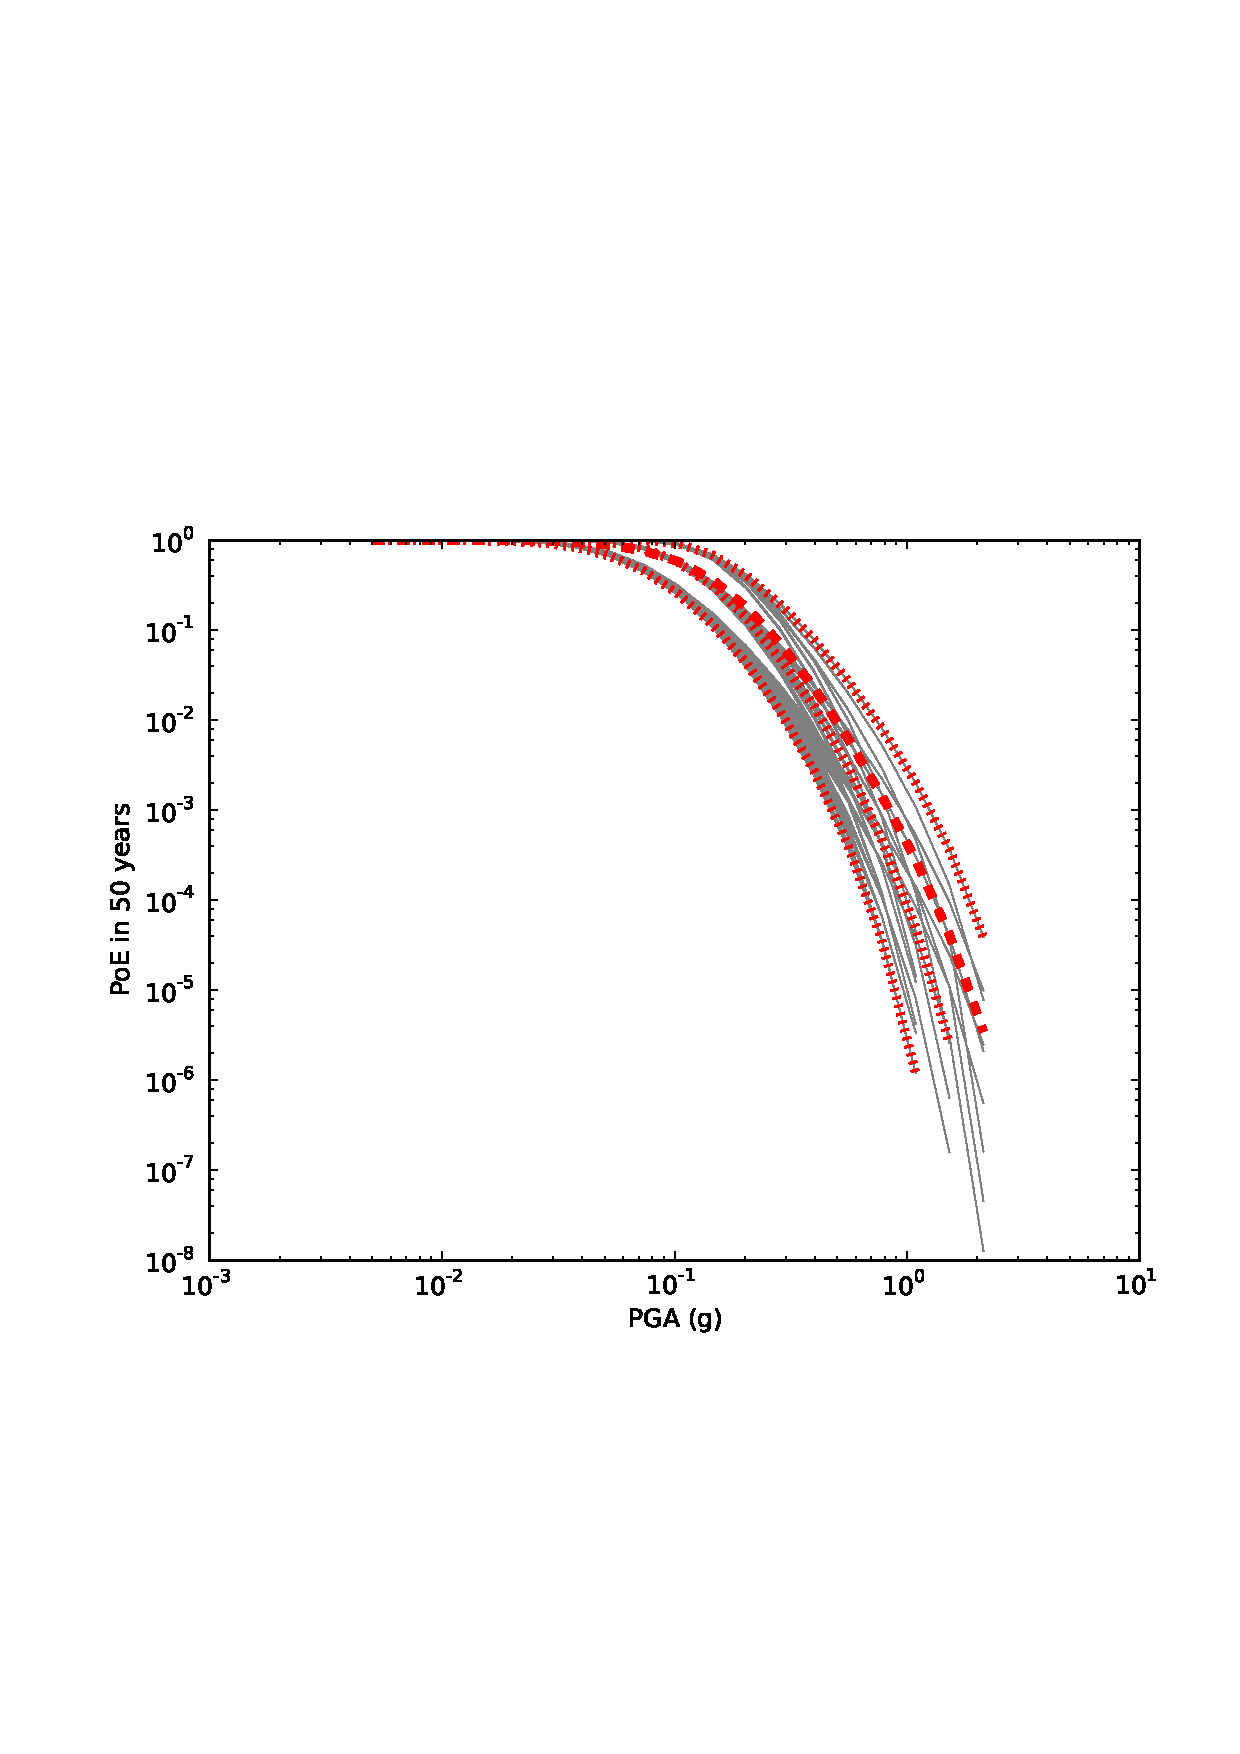
\includegraphics[width=9cm]{./figures/hazard/hazard-curves-ltcase2.pdf}}
\caption{Hazard curves as obtained from the LogicTreeCase2 demo. Solid gray lines represent individual hazard curves from the different
logic tree path (a total of 324 curves). The red dashed line represents the mean hazard curve, while the red dotted lines depict the quantile levels
(0.15, 0.5, 0.95).}
\label{fig:hazard_curves}
\end{figure}

LogicTreeCase3ClassicalPSHA illustrates an example of logic tree defining relative uncertainties on G-R maximum magnitude and b value.
A single source model is considered containing two sources belonging to different tectonic region types and both characterized by a G-R 
magnitude frequency distribution. The source model logic tree is as follows:
\begin{Verbatim}[frame=single, commandchars=\\\{\}, fontsize=\normalsize]
<?xml version="1.0" encoding="UTF-8"?>
<nrml xmlns:gml="http://www.opengis.net/gml"
      xmlns="http://openquake.org/xmlns/nrml/0.4">
    <logicTree logicTreeID="lt1">

        <logicTreeBranchingLevel branchingLevelID="bl1">
            <logicTreeBranchSet uncertaintyType="sourceModel"
                                branchSetID="bs1">
                <logicTreeBranch branchID="b11">
                    <uncertaintyModel>
                     source_model.xml
                    </uncertaintyModel>
                    <uncertaintyWeight>1.0</uncertaintyWeight>
                </logicTreeBranch>
            </logicTreeBranchSet>
        </logicTreeBranchingLevel>

        <logicTreeBranchingLevel branchingLevelID="bl2">
            <logicTreeBranchSet uncertaintyType="bGRRelative"
                                branchSetID="bs21">
                <logicTreeBranch branchID="b21">
                    <uncertaintyModel>+0.1</uncertaintyModel>
                    <uncertaintyWeight>0.333</uncertaintyWeight>
                </logicTreeBranch>
                <logicTreeBranch branchID="b22">
                    <uncertaintyModel>0.0</uncertaintyModel>
                    <uncertaintyWeight>0.333</uncertaintyWeight>
                </logicTreeBranch>
                <logicTreeBranch branchID="b23">
                    <uncertaintyModel>-0.1</uncertaintyModel>
                    <uncertaintyWeight>0.334</uncertaintyWeight>
                </logicTreeBranch>
            </logicTreeBranchSet>
        </logicTreeBranchingLevel>

        <logicTreeBranchingLevel branchingLevelID="bl3">
            <logicTreeBranchSet uncertaintyType="maxMagGRRelative"
                                branchSetID="bs31">
                <logicTreeBranch branchID="b31">
                    <uncertaintyModel>0.0</uncertaintyModel>
                    <uncertaintyWeight>0.333</uncertaintyWeight>
                </logicTreeBranch>
                <logicTreeBranch branchID="b32">
                    <uncertaintyModel>+0.5</uncertaintyModel>
                    <uncertaintyWeight>0.333</uncertaintyWeight>
                </logicTreeBranch>
                <logicTreeBranch branchID="b33">
                    <uncertaintyModel>+1.0</uncertaintyModel>
                    <uncertaintyWeight>0.334</uncertaintyWeight>
                </logicTreeBranch>
            </logicTreeBranchSet>
        </logicTreeBranchingLevel>

    </logicTree>
</nrml>
\end{Verbatim}
After the first branching level defining the source model, two additional branching levels are defined, one defining
relative uncertainties on b value (\texttt{bGRRelative} applied consistently to all sources in the source model)
and the second uncertainties on maximum magnitude (\texttt{maxMagGRRelative}). Similarly to the other cases,
two GMPEs are considered for each tectonic region type and therefore the total number of logic tree path is 36
(1 source model x 3 b value increments x 3 maximum magnitude increments x 2 GMPE for Active x 2 GMPEs for Stable)

\subsubsection{Event Based PSHA}
A demo showing an example of Event Based calculation is provided with the following configuration file:
\begin{Verbatim}[frame=single, commandchars=\\\{\}, fontsize=\normalsize]
[general]

description = Event Based PSHA using Area Source
calculation_mode = event_based
random_seed = 23

[geometry]

sites = 0.5 -0.5

[logic_tree]

number_of_logic_tree_samples = 0

[erf]

rupture_mesh_spacing = 2
width_of_mfd_bin = 0.1
area_source_discretization = 5.0

[site_params]

reference_vs30_type = measured
reference_vs30_value = 600.0
reference_depth_to_2pt5km_per_sec = 5.0
reference_depth_to_1pt0km_per_sec = 100.0

[calculation]

source_model_logic_tree_file = source_model_logic_tree.xml
gsim_logic_tree_file = gmpe_logic_tree.xml
investigation_time = 50.0
intensity_measure_types_and_levels = {"PGA": [...]}
truncation_level = 3
maximum_distance = 200.0

[event_based_params]

ses_per_logic_tree_path = 100
ground_motion_correlation_model =
ground_motion_correlation_params =

[output]

export_dir = ...
ground_motion_fields = true
hazard_curves_from_gmfs = true
mean_hazard_curves = false
quantile_hazard_curves =
hazard_maps = true
poes = 0.1
\end{Verbatim}
The source model consist of one source (area). 100 stochastic event sets are generated (\texttt{ses\_\-per\_\-logic\_\-tree\_\-path = 100}) (an example can be seen
in figure \ref{fig:ses}). Ground motion fields are computed (\texttt{ground\_\-motion\_\-fields = true}, figure \ref{fig:gmfs}) and also hazard curves from ground motion fields are
extracted (\texttt{hazard\_\-curves\_\-from\_\-gmfs = true}).
Corresponding hazard maps for 0.1 probability are additionally calculated (\texttt{hazard\_\-maps = true})

\begin{figure} 
\centering 
\subcaptionbox{}
{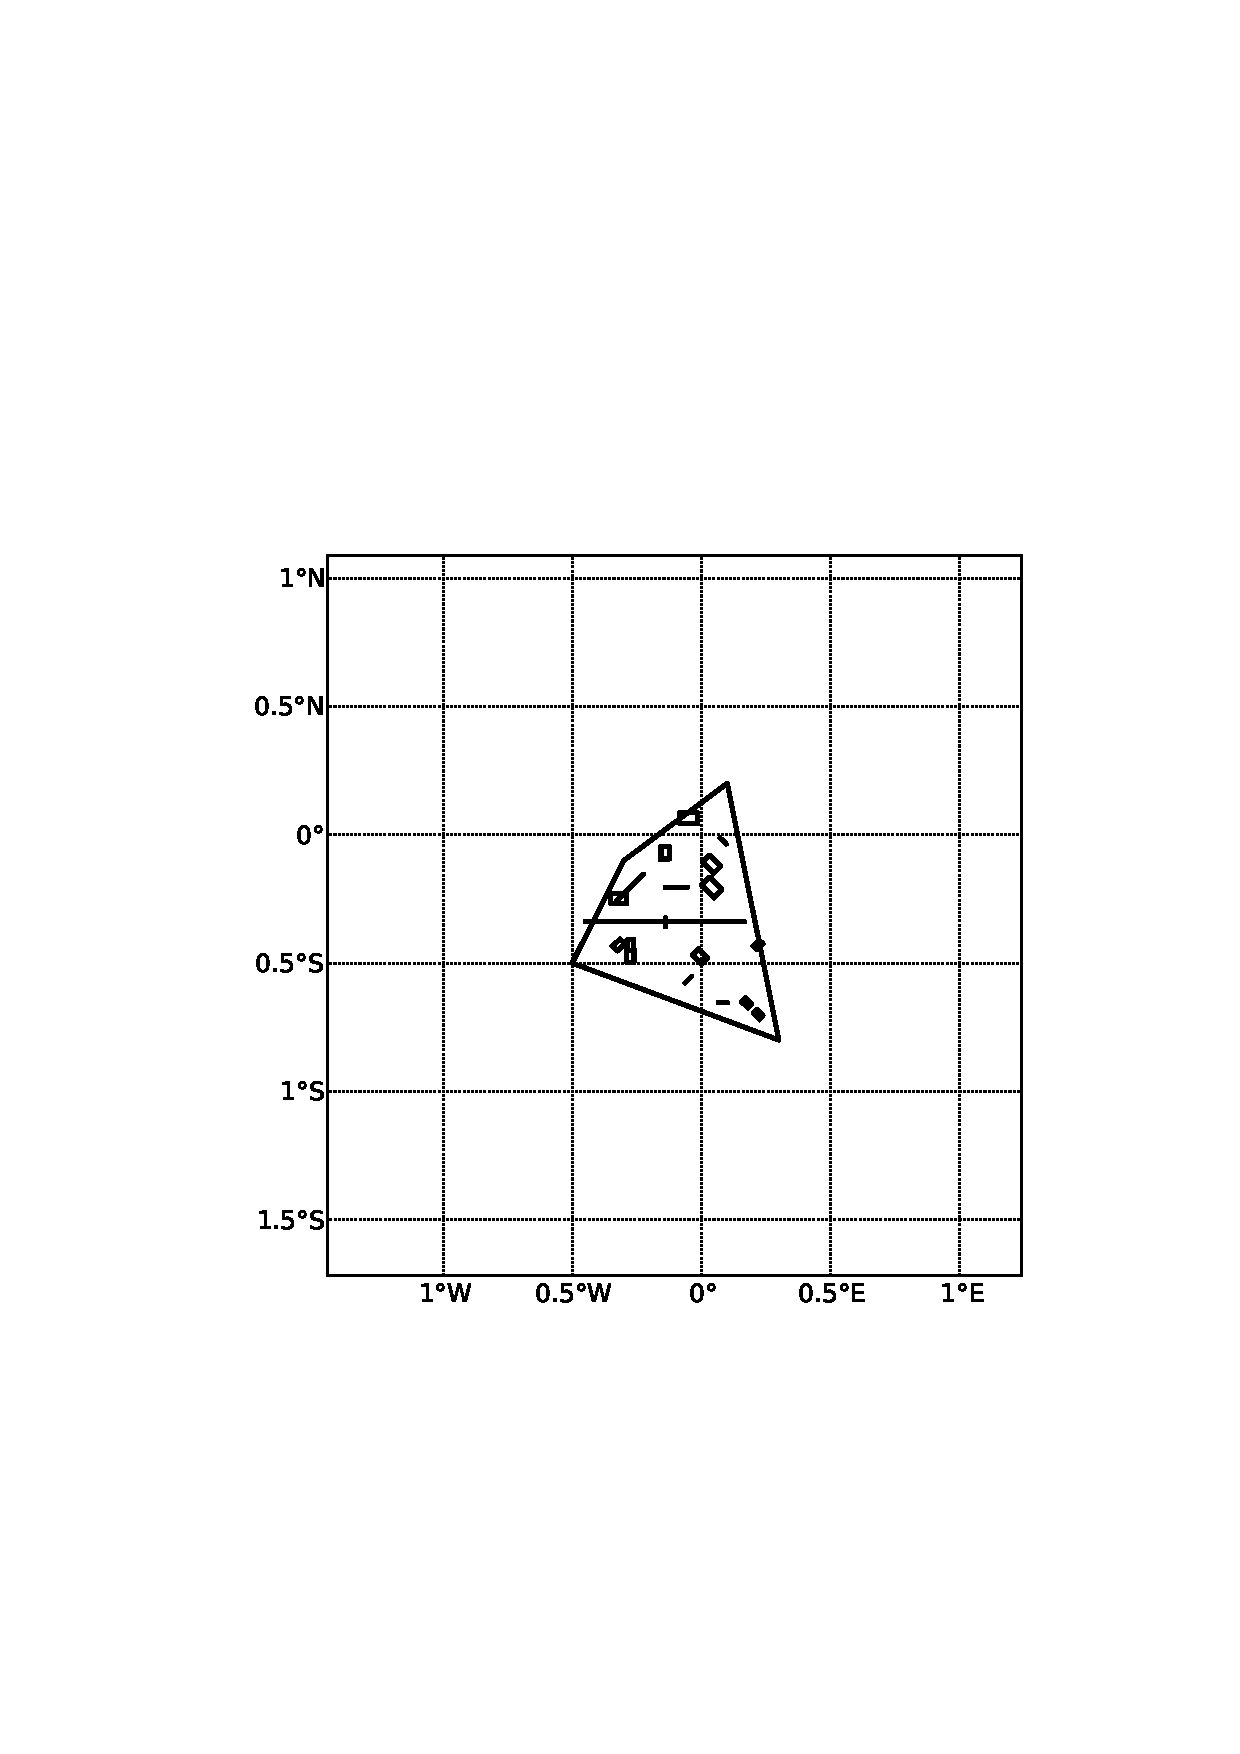
\includegraphics[width=9cm]{./figures/hazard/ses.pdf}} 
\caption{A stochastic event set generated in the event based PSHA demo. The area source defines a nodal plane distribution which distributes events among vertical and
dipping (50 degrees) faults with equal weights. Vertical ruptures are then distributed equally in the range 0-180 degrees while the dipping ones in the range 0-360, both
with a step of 45 degrees.}
\label{fig:ses}
\end{figure}

\begin{figure} 
\centering 
\subcaptionbox{}
{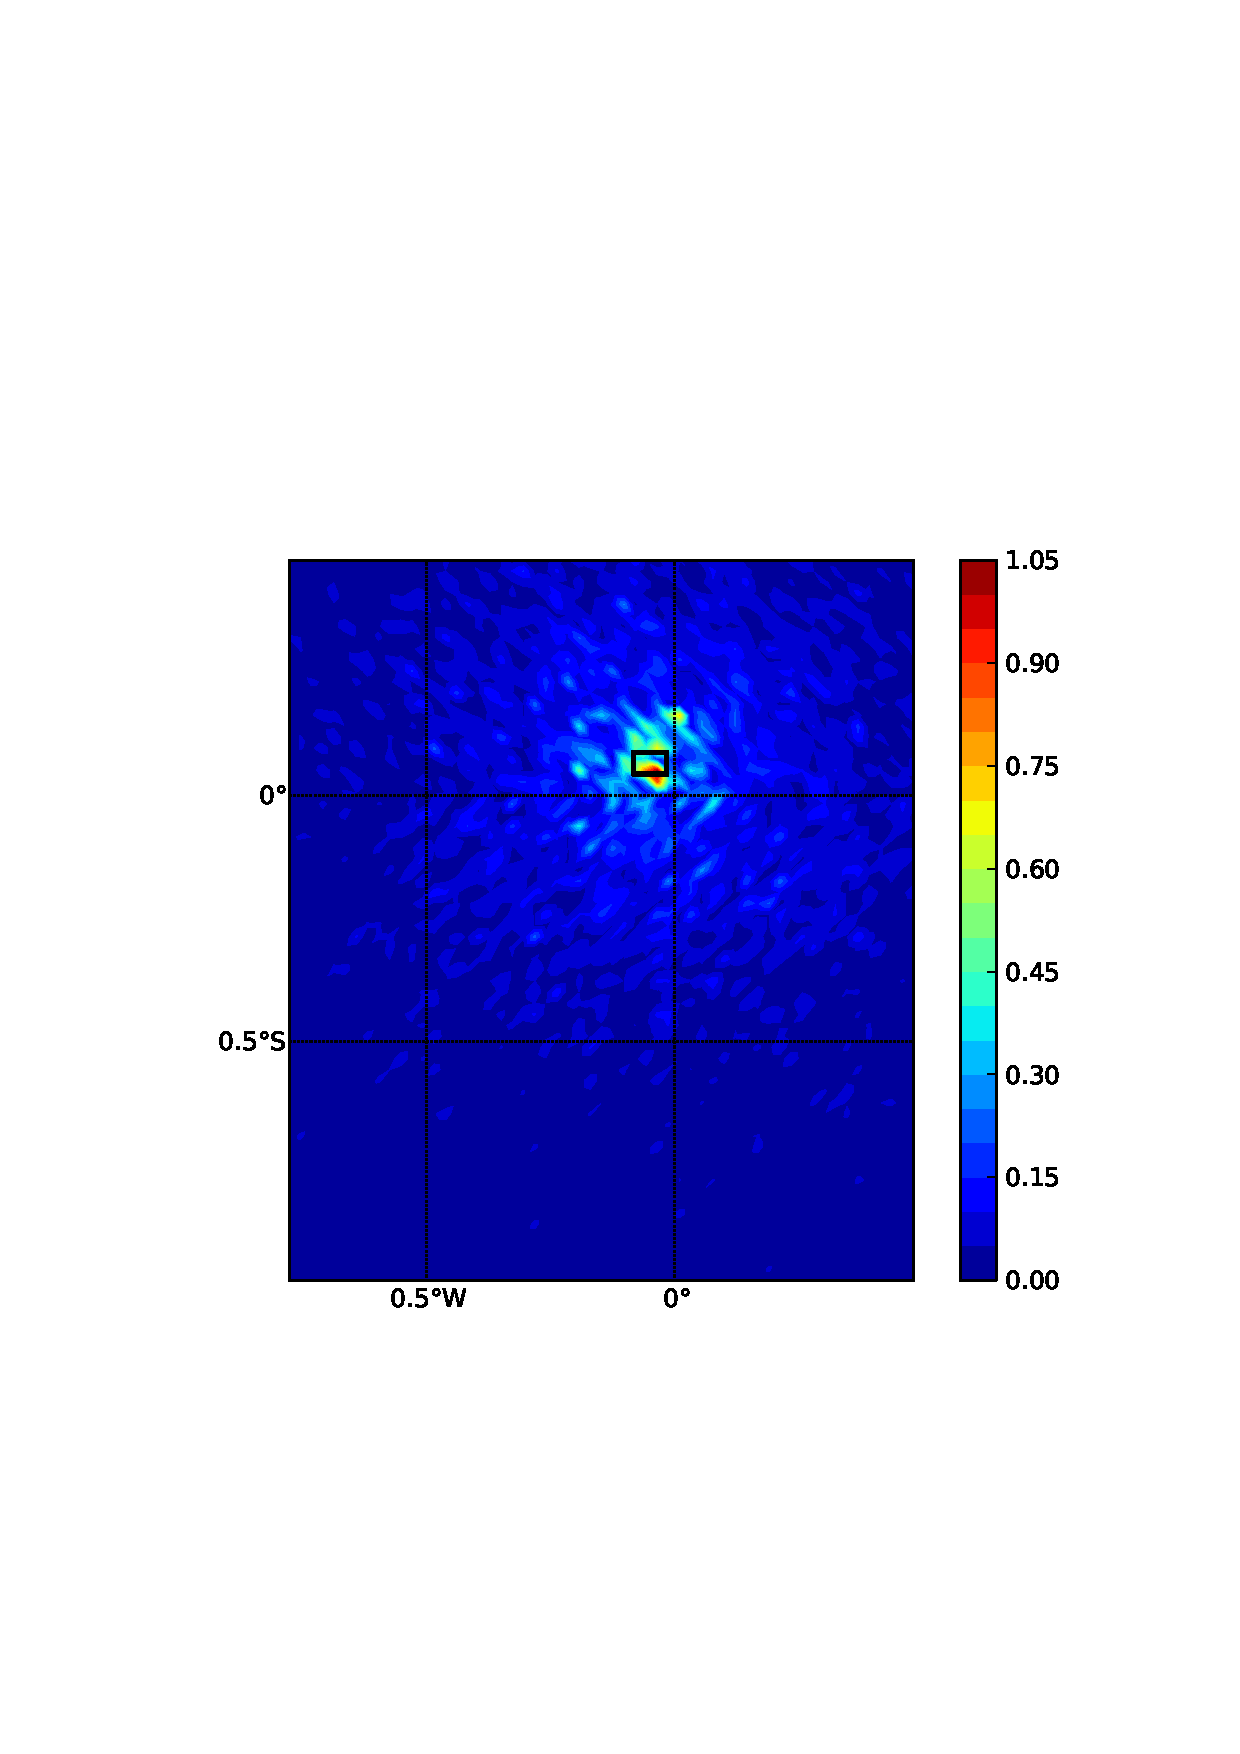
\includegraphics[width=6cm]{./figures/hazard/gmf-no-corr.pdf}} 
\subcaptionbox{}
{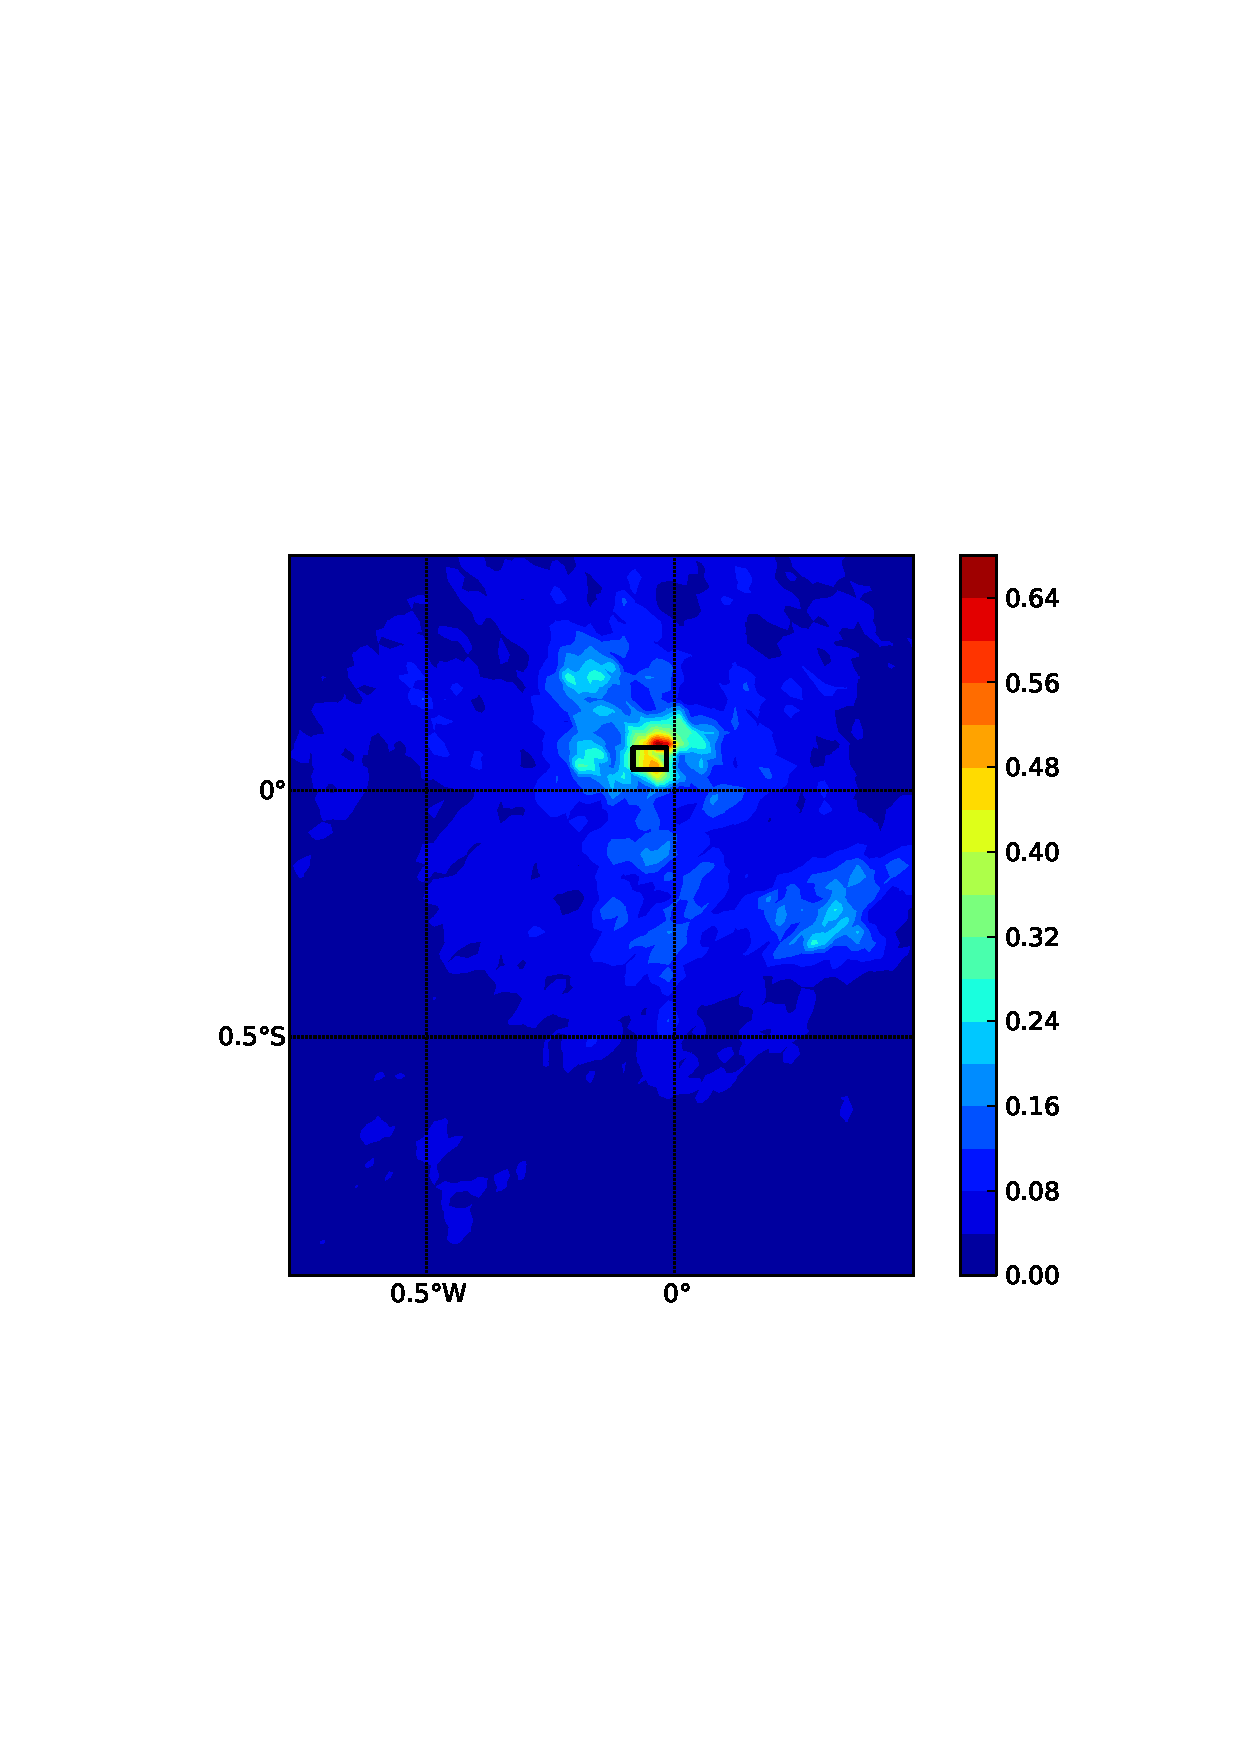
\includegraphics[width=6cm]{./figures/hazard/gmf-corr.pdf}} 
\caption{Ground motion fields (PGA) with no spatial correlations (a) and with spatial correlation (b)}
\label{fig:gmfs}
\end{figure}

\subsubsection{Disaggregation}
An example of disaggregation calculation is given considering a source model consisting of two sources (area and simple fault) belonging to two different tectonic region types.
The calculation is described by the following configuration file:
\begin{Verbatim}[frame=single, commandchars=\\\{\}, fontsize=\normalsize]
[general]

description = ...
calculation_mode = disaggregation
random_seed = 23

[geometry]

sites = 0.5 -0.5

[logic_tree]

number_of_logic_tree_samples = 0

[erf]

rupture_mesh_spacing = 2
width_of_mfd_bin = 0.1
area_source_discretization = 5.0

[site_params]

reference_vs30_type = measured
reference_vs30_value = 600.0
reference_depth_to_2pt5km_per_sec = 5.0
reference_depth_to_1pt0km_per_sec = 100.0

[calculation]

source_model_logic_tree_file = source_model_logic_tree.xml
gsim_logic_tree_file = gmpe_logic_tree.xml
investigation_time = 50.0
intensity_measure_types_and_levels = {"PGA": [...]}
truncation_level = 3
maximum_distance = 200.0

[disaggregation]

poes_disagg = 0.1
mag_bin_width = 1.0
distance_bin_width = 10.0
coordinate_bin_width = 0.2
num_epsilon_bins = 3

[output]

export_dir = ...
\end{Verbatim}
Disaggregation matrices are computed for a single site (located between the two sources) for a ground motion value corresponding to a probability value equal to 0.1
(\texttt{poes\_\-disagg = 0.1}). Magnitude values are classified in one magnitude unit bins (\texttt{mag\_\-bin\_\-width = 1.0}), distances in bins of 10 km
(\texttt{distance\_\-bin\_\-width = 10.0}), coordinates in bins of 0.2 degrees (\texttt{coordinate\_\-bin\_\-width = 0.2}). 3 epsilons bins are considered (\texttt{num\_\-epsilon\_\-bins = 3}).

\begin{comment}
The demo allows to compute 

\section{Demo 01 - Classical PSHA}

% -----------------------------------------------------------------------------
\section{Demo 02 - Classical PSHA: simple logic tree}
This demo contains simple logic tree structures accounting for epistemic
uncertainties in the seismic source and ground motion intensity models.

The seismic source model incorporates epistemic uncertainty about the 
value of the maximum magnitude of the magnitude-frequency distribution 
used.
%
The ground motion intensity model includes uncertainty about the ground
motion prediction equations to be used in the calculation of hazard.

Given that the overall structure of the logic tree is not particularly
complex and assuming that uncertainties are fully correlated we decide 
to compute all the possible realisations of the logic tree by fixing 
the \texttt{number\_\-of\_\-logic\_\-tree\_\-samples} parameter in the 
configuration file to zero.
\begin{Verbatim}[frame=single, commandchars=\\\{\}, fontsize=\normalsize]
[logic_tree]
number_of_logic_tree_samples = 0
\end{Verbatim}

Let's now run the OpenQuake:
\begin{Verbatim}[frame=single, fontsize=\normalsize]
user@ubuntu:~/demos/classical_psha_simple_lt$ oq-engine \ 
--rh job_1strike.ini 
\end{Verbatim}

This is the list of results that we get at the end of this calculation:
\begin{Verbatim}[frame=single, commandchars=\\\{\}, fontsize=\normalsize]
Calculation 8 results:
id | output_type | name
5 | hazard_curve | hc-rlz-10
6 | hazard_curve | hc-rlz-7
7 | hazard_curve | hc-rlz-8
8 | hazard_curve | hc-rlz-9
9 | hazard_curve | hc-rlz-11
10 | hazard_curve | hc-rlz-12
11 | hazard_map | hazard-map(0.1)-PGA-rlz-10
12 | hazard_map | hazard-map(0.1)-PGA-rlz-7
13 | hazard_map | hazard-map(0.1)-PGA-rlz-8
14 | hazard_map | hazard-map(0.1)-PGA-rlz-9
15 | hazard_map | hazard-map(0.1)-PGA-rlz-11
16 | hazard_map | hazard-map(0.1)-PGA-rlz-12
\end{Verbatim}
OpenQuake produced six hazard curves and six hazard maps i.e. one
result for each leaf of the logic tree. 
\end{comment}
   \cleardoublepage

% ------------------------------------------------------ Part III: Risk Module -
\thispagestyle{empty}
\part{Risk}

\chapterimage{figures/chapter_head_2.pdf} % Chapter heading image
\chapter{Introduction to the Risk Module}
   \label{chap:riskintro}
	\index{OpenQuake-engine!risk}

The seismic risk results are being calculated using the OpenQuake risk library
(oq-risklib), an open-source suite of tools for seismic risk assessment and
loss estimation. This library is written in the Python programming language
and available in the form of a ``developers'' release, that can be executed
through a command line interface. The code of the library can be found on a
public repository at GitHub at the following address
\href{http://github.com/gem/oq-risklib}{http://github.com/gem/oq-risklib}.

The risk component of the OpenQuake-engine can compute both scenario-based and
probabilistic seismic damage and risk using various approaches. The following
types of analysis are currently supported:

\begin{itemize}

    \item \textit{Scenario Damage Assessment}, allowing the calculation of
	damage distribution statistics for a portfolio of buildings from a single
	earthquake rupture scenario taking into account aleatory and epistemic
	ground-motion variability.

	\item \textit{Scenario Risk Assessment}, for the calculation of individual 
	asset and portfolio loss statistics due to a single earthquake 
	rupture scenario taking into account aleatory and epistemic ground-motion 
	variability. Correlation in the vulnerability of different assets of the 
	same typology can also be taken into consideration.

	\item \textit{Classical Probabilistic Seismic Damage Analysis}, for 
	calculation of damage state probabilities over a specified time period,  
	and probabilistic collapse maps, starting from the hazard curves 
	computed following the classical integration procedure (\cite{cornell1968}, 
	\citet{mcguire1976}) as formulated by \cite{field2003}.

    \item \textit{Classical Probabilistic Seismic Risk Analysis}, allowing
	calculation of loss curves and loss maps, starting from the hazard curves 
	computed following the classical integration procedure (\cite{cornell1968}, 
	\citet{mcguire1976}) as formulated by \cite{field2003}.

	\item \textit{Event-Based Probabilistic Seismic Risk Analysis}, 
	allowing calculation of event-loss tables starting from stochastic event sets.
	Other results such as loss-exceedance curves, probabilistic loss maps, 
	average annual losses, and insured loss statistics can be obtained by post-
	processing the event-loss tables.

	\item \textit{Retrofit Benefit-Cost Ratio Analysis}, which is useful in 
	estimating the net-present value of the potential benefits of performing  
	retrofitting for a portfolio of assets (in terms of decreased losses in 
	seismic events), measured relative to the upfront cost of retrofitting.

\end{itemize}

Each calculation workflow has a modular structure, so that intermediate
results can be exported and analyzed. Moreover, each calculator can be
extended independently of the others so that additional calculation options
and methodologies can be easily introduced, without affecting the overall
calculation workflow.

The following sections describe the basic inputs required for a risk
calculation, including exposure models, fragility models, consequence models,
and vulnerability models. The final section of this chapter describes each of
the above workflows in detail.

For further information regarding the theoretical background of the
methodologies used for each calculator, users are referred to the OpenQuake-
engine Book (Risk).


\section{Exposure models}
\label{sec:exposure}
All risk calculators in the OpenQuake-engine require an \gls{exposure model}
that needs to be provided in the NRML format. The information included in an
exposure model comprises a metadata section, followed by data regarding each
individual asset in the portfolio.

There are a number of parameters that compose the metadata, and provides
general information regarding the \glspl{asset} within the \gls{exposure
model}, as described below:

\begin{itemize}

    \item \Verb+id+: a unique key used to identify the gls{exposure model};

    \item \Verb+category+: a string used to define the type of glspl{asset}
    being stored (e.g: buildings, lifelines);

    \item \Verb+taxonomySource+: attribute used to define the gls{taxonomy}
    being used to classify the glspl{asset};

    \item \Verb+description+: brief string with further information about the
    \gls{exposure model};

\end{itemize}

The information in the metadata section is common to all of the assets in the
portfolio and needs to be incorporated at the beginning of every exposure
model file as illustrated in the following example:

\begin{Verbatim}[frame=single, commandchars=\\\{\}, samepage=false]
<?xml version="1.0" encoding="UTF-8"?>
<nrml xmlns="http://openquake.org/xmlns/nrml/0.5">
<\textcolor{red}{exposureModel} id="exposure_model"
      category="buildings"
      taxonomySource="GEM taxonomy">
    <\textcolor{green}{description}>Buildings in Pavia</\textcolor{green}{description}>
...
\end{Verbatim}


The NRML schema for the exposure model allows the definition of various types
of costs (structural cost, nonstructural cost, contents cost, business
interruption cost). Further explanation regarding the cost types and values
used to define the exposure elements can be found in the OpenQuake-engine Book 
(Risk).

The way the information about the characteristics of the \glspl{asset} in an
\gls{exposure model} are stored can vary strongly depending on how and why the
data was compiled. As an example, if national census information is used to
estimated the distribution of assets in a given region, it is likely that the
number of buildings within a given geographical area will be used to define
the dataset, and will be used for estimating the number of collapsed buildings
for a scenario earthquake. On the other hand, if simplified methodologies
based on proxy data such as population distribution are used to develop the
exposure model, then it is likely that the built up area or economic cost of
each building typology will be directly derived, and will be used for the
estimation of economic losses. Thus, the following set of attributes exist
within the schema for the exposure model:

\begin{itemize}

    \item \Verb+number+: number of units of a given gls{asset} at a given
    location;

    \item \Verb+area+: area of the gls{asset}, at a given location;

    \item \Verb+cost+: structural replacement cost of the gls{asset} at a given
    location;

\end{itemize}

The set of required attributes depends on what and how a user wants to store
the information about the assets in the exposure model. While the attribute
\\Verb+number+ might be a rather simple parameter, the other two (area and
cost) can be ambiguous, as different ways to define them might be used. With
regards to the attribute \\Verb+area+, one can either choose to provide the
aggregated built up area of the \glspl{asset} per location or the average
built up area for a single building unit (noting that an \gls{asset} might be
made up of a number of individual buildings). Similarly, the \\Verb+cost+ can
also be defined as the aggregated structural replacement cost, the cost of
replacing a single unit or even the structural replacement cost per unit of
area. For the purposes of performing a retrofitting benefit/cost analysis, it
is also necessary to define the retrofitting cost (\\Verb+reco+). The
combination between the possible options in which these three attributes can
be defined leads to four ways of storing the information about the assets. For
each of these cases a brief explanation and example is provided in this
section.

\paragraph{Example 1}
This example is comprised of an \gls{exposure model} in which the aggregated cost (structural, nonstructural, contents and business interruption) of the buildings of each taxonomy for a set of locations is directly provided. Thus, in order to indicate how the various costs will be defined, the following information needs to be stored in the exposure model file:

\begin{Verbatim}[frame=single, commandchars=\\\{\}, samepage=false]
...
 <\textcolor{green}{conversions}>
  <\textcolor{blue}{costTypes}>
   <\textcolor{magenta}{costType} name="structural" type="aggregated" unit="EUR">
   <\textcolor{magenta}{costType} name="non_structural" type="aggregated" unit="EUR" />
   <\textcolor{magenta}{costType} name="business_interruption" type="aggregated" 
                                                      unit="EUR"/>
   <\textcolor{magenta}{costType} name="contents" type="aggregated" unit="EUR"/>
  </\textcolor{blue}{costTypes}>
 </\textcolor{green}{conversions}>
...
\end{Verbatim}

In this case, the cost \\Verb+type+ of each component as been defined as \\Verb+aggregated+. Once the way in which each cost is going to be defined has been established, the values for each asset can be stored according to the following format:

\begin{Verbatim}[frame=single, commandchars=\\\{\}, samepage=false]
...
 <\textcolor{green}{assets}>
  <\textcolor{blue}{asset} id="asset_01" taxonomy="RC/DMRF-D/LR">
   <\textcolor{magenta}{location} lon="9.15" lat="45.17" />
   <\textcolor{magenta}{costs}>
    <cost type="structural" value="1500"/>
    <cost type="non_structural" value="2500"/>
    <cost type="contents" value="1200"/>
    <cost type="business_interruption" value="400"/>
   </\textcolor{magenta}{costs}>
  </\textcolor{blue}{asset}>
...
  <\textcolor{blue}{asset} id="asset_99"  taxonomy="RC/DMRF-D/HR">
   <\textcolor{magenta}{location} lon="9.15" lat="45.12" />
   <\textcolor{magenta}{costs}>
    <cost type="structural" value="2500"/>
    <cost type="non_structural" value="2100"/>
    <cost type="contents" value="1900"/>
    <cost type="business_interruption" value="40"/>
   </\textcolor{magenta}{costs}>
  </\textcolor{blue}{asset}>
 </\textcolor{green}{assets}>
</\textcolor{red}{exposureModel}>
</nrml>
\end{Verbatim}

Each \gls{asset} is uniquely identified by its \\Verb+id+, which is used by the OpenQuake-engine to relate each asset with the associated results (e.g. loss exceedance curves). Then, a pair of coordinates (latitude and longitude) for a \\Verb+location+ where the asset is assumed to exist is defined. \footnote{Within the OpenQuake-engine, longitude and latitude coordinates are internally rounded to a precision of 5 digits after the decimal point.} Each asset must be classified according to a \\Verb+taxonomy+, so that the OpenQuake-engine is capable of employing the appropriate \gls{vulnerability function} or \gls{fragility function} in the risk calculations. Finally, the cost values of each \\Verb+type+ are stored within the \\Verb+costs+ attribute. In this example, the aggregated value for all units (within a given asset) at each location is provided directly, so there is no need to define other attributes such as \\Verb+number+ or \\Verb+area+. This mode of representing an exposure model is probably the simplest one.

\paragraph{Example 2}
In this example an \gls{exposure model} containing the number of units (buildings) and the associated costs per unit of each building typology is presented.

\begin{Verbatim}[frame=single, commandchars=\\\{\}, samepage=false]
...
 <\textcolor{green}{conversions}>
  <\textcolor{blue}{costTypes}>
   <\textcolor{magenta}{costType} name="structural" type="per_unit" unit="EUR">
   <\textcolor{magenta}{costType} name="non_structural" type="per_unit" unit="EUR" />
   <\textcolor{magenta}{costType} name="business_interruption" type="per_unit" 
                                                      unit="EUR"/>
   <\textcolor{magenta}{costType} name="contents" type="per_unit" unit="EUR"/>
  </\textcolor{blue}{costTypes}>
 </\textcolor{green}{conversions}>
...
\end{Verbatim}

For this case, the cost \\Verb+type+ has been set to \\Verb+per_unit+. Then, the information from each asset can be stored following the format below:

\begin{Verbatim}[frame=single, commandchars=\\\{\}, samepage=false]
...
 <\textcolor{green}{assets}>
  <\textcolor{blue}{asset} id="asset_01" number="10" taxonomy="RC/DMRF-D/LR">
   <\textcolor{magenta}{location} lon="9.15" lat="45.17" />
   <\textcolor{magenta}{costs}>
    <cost type="structural" value="150"/>
    <cost type="non_structural" value="250"/>
    <cost type="contents" value="120"/>
    <cost type="business_interruption" value="40"/>
   </\textcolor{magenta}{costs}>
  </\textcolor{blue}{asset}>
...
  <\textcolor{blue}{asset} id="asset_99" number="20" taxonomy="RC/DMRF-D/HR">
   <\textcolor{magenta}{location} lon="9.15" lat="45.12" />
   <\textcolor{magenta}{costs}>
    <cost type="structural" value="125"/>
    <cost type="non_structural" value="105"/>
    <cost type="contents" value="95"/>
    <cost type="business_interruption" value="20"/>
   </\textcolor{magenta}{costs}>
  </\textcolor{blue}{asset}>
 </\textcolor{green}{assets}>
</\textcolor{red}{exposureModel}>
</nrml>
\end{Verbatim}

In this example, the various costs for each asset is not provided directly, as happened in the previous example. In order to carry out the risk calculations in which the economic cost of each asset is required, the OpenQuake-engine multiplies, for each asset, the number of units (buildings) by the ``per unit'' replacement cost. Note that in this case, there is no need to specify the attribute \\Verb+area+.

\paragraph{Example 3}
This example is comprised of an \gls{exposure model} containing the built up area of each building typology for a set of locations, and the associated costs per area.

\begin{Verbatim}[frame=single, commandchars=\\\{\}, samepage=false]
...
 <\textcolor{green}{conversions}>
  <\textcolor{blue}{area} type="aggregated" unit="square meters"/>
  <\textcolor{blue}{costTypes}>
   <\textcolor{magenta}{costType} name="structural" type="per_area" unit="EUR">
   <\textcolor{magenta}{costType} name="non_structural" type="per_area" unit="EUR" />
   <\textcolor{magenta}{costType} name="business_interruption" type="per_area" 
                                                      unit="EUR"/>
   <\textcolor{magenta}{costType} name="contents" type="per_area" unit="EUR"/>
  </\textcolor{blue}{costTypes}>
 </\textcolor{green}{conversions}>
...
\end{Verbatim}

In order to compile an \gls{exposure model} with this structure, it is required to set the cost \\Verb+type+ to \\Verb+per_area+. In addition, it is also necessary to specify if the \\Verb+area+ that is being store represents the aggregated area of number of units within an asset, or the average area of a single unit. In this particular case, the \\Verb+area+ that is being stored is the aggregated built up area per asset, and thus this attribute was set to \\Verb+aggregated+.

\begin{Verbatim}[frame=single, commandchars=\\\{\}, samepage=false]
...
 <\textcolor{green}{assets}>
  <\textcolor{blue}{asset} id="asset_01" area="50" taxonomy="RC/DMRF-D/LR">
   <\textcolor{magenta}{location} lon="9.15" lat="45.17" />
   <\textcolor{magenta}{costs}>
    <cost type="structural" value="100"/>
    <cost type="non_structural" value="200"/>
    <cost type="contents" value="90"/>
    <cost type="business_interruption" value="10"/>
   </\textcolor{magenta}{costs}>
  </\textcolor{blue}{asset}>
...
  <\textcolor{blue}{asset} id="asset_99" area ="60" taxonomy="RC/DMRF-D/HR">
   <\textcolor{magenta}{location} lon="9.15" lat="45.12" />
   <\textcolor{magenta}{costs}>
    <cost type="structural" value="150"/>
    <cost type="non_structural" value="250"/>
    <cost type="contents" value="50"/>
    <cost type="business_interruption" value="30"/>
   </\textcolor{magenta}{costs}>
  </\textcolor{blue}{asset}>
 </\textcolor{green}{assets}>
</\textcolor{red}{exposureModel}>
</nrml>
\end{Verbatim}

Once again, the OpenQuake-engine needs to carry out some calculations in order to compute the different costs per asset. In this case, this value is computed by multiplying the aggregated built up \\Verb+area+ of each building typology by the associated cost per unit of area. Notice that in this case, there is no need to specify the attribute \\Verb+number+.

\paragraph{Example 4}
This example is comprised of an \gls{exposure model} containing the number of buildings for each location, the average built up area per building unit and the associated costs per area.

\begin{Verbatim}[frame=single, commandchars=\\\{\}, samepage=false]
...
 <\textcolor{green}{conversions}>
  <\textcolor{blue}{area} type="per_asset" unit="square meters"/>
  <\textcolor{blue}{costTypes}>
   <\textcolor{magenta}{costType} name="structural" type="per_area" unit="EUR">
   <\textcolor{magenta}{costType} name="non_structural" type="per_area" unit="EUR" />
   <\textcolor{magenta}{costType} name="business_interruption" type="per_area" 
                                                      unit="EUR"/>
   <\textcolor{magenta}{costType} name="contents" type="per_area" unit="EUR"/>
  </\textcolor{blue}{costTypes}>
 </\textcolor{green}{conversions}>
...
\end{Verbatim}

Similarly to what was described in the previous example, the various costs \\Verb+type+ also need to be establish as \\Verb+per_area+, but the \\Verb+type+ of area is now defined as \\Verb+per_unit+.

\begin{Verbatim}[frame=single, commandchars=\\\{\}, samepage=false]
...
 <\textcolor{green}{assets}>
  <\textcolor{blue}{asset} id="asset_01" number="5" area="50" taxonomy="RC/DMRF-D/LR">
   <\textcolor{magenta}{location} lon="9.15" lat="45.17" />
   <\textcolor{magenta}{costs}>
    <cost type="structural" value="100"/>
    <cost type="non_structural" value="200"/>
    <cost type="contents" value="90"/>
    <cost type="business_interruption" value="10"/>
   </\textcolor{magenta}{costs}>
  </\textcolor{blue}{asset}>
...
  <\textcolor{blue}{asset} id="asset_99" number="8" area ="60" taxonomy="RC/DMRF-D/HR">
   <\textcolor{magenta}{location} lon="9.15" lat="45.12" />
   <\textcolor{magenta}{costs}>
    <cost type="structural" value="150"/>
    <cost type="non_structural" value="250"/>
    <cost type="contents" value="50"/>
    <cost type="business_interruption" value="30"/>
   </\textcolor{magenta}{costs}>
  </\textcolor{blue}{asset}>
 </\textcolor{green}{assets}>
</\textcolor{red}{exposureModel}>
</nrml>
\end{Verbatim}

In this example, the OpenQuake-engine will make use of all the parameters to estimate the various costs of each asset, by multiplying the number of buildings by its average built up area, and then by the respective cost per unit of area.

\paragraph{Example 5}
In this example, additional information will be included, which is required for other risk analysis besides loss estimation, such as the calculation of insured losses or benefit/cost analysis. For the former assessment, it is necessary to establish how the insured limit and deductible is going to be define, according to the format below. 
\begin{Verbatim}[frame=single, commandchars=\\\{\}, samepage=false]
...
 <\textcolor{green}{conversions}>
  <\textcolor{blue}{costTypes}>
   <\textcolor{magenta}{costType} name="structural" type="aggregated" unit="EUR">
   <\textcolor{magenta}{costType} name="non_structural" type="aggregated" unit="EUR" />
   <\textcolor{magenta}{costType} name="business_interruption" type="aggregated" 
                                                      unit="EUR"/>
   <\textcolor{magenta}{costType} name="contents" type="aggregated" unit="EUR"/>
  </\textcolor{blue}{costTypes}>
  <\textcolor{blue}{deductible} isAbsolute="false"/>
  <\textcolor{blue}{insuranceLimit} isAbsolute="false"/>
 </\textcolor{green}{conversions}>
...
\end{Verbatim}

In this example, both the insurance limit and the deductible were defined as a fraction of the costs, by setting the attribute \\Verb+isAbsolute+ to \\Verb+false+. On the other hand, a user could define one or both of these parameters as the absolute threshold, by setting the aforementioned attribute to \\Verb+true+. Then, for each type of cost, the limit and deductible value can be stored for each asset.
Moreover, in order to perform a benefit/cost assessment, it is also fundamental to indicate the retrofitting cost. This parameter is handled in the same manner as the structural cost, and it should be stored according to the following structure.

\begin{Verbatim}[frame=single, commandchars=\\\{\}, samepage=false]
...
 <\textcolor{green}{assets}>
  <\textcolor{blue}{asset} id="asset_01" taxonomy="RC/DMRF-D/LR">
   <\textcolor{magenta}{location} lon="9.15" lat="45.17" />
   <\textcolor{magenta}{costs}>
    <cost type="structural" value="1500" deductible=".05" 
                insuranceLimit="0.9" retrofitted="200"/>
    <cost type="non_structural" value="2500" deductible=".1" 
                insuranceLimit="0.8"/>
    <cost type="contents" value="1200" deductible=".2" 
                insuranceLimit="0.6"/>
    <cost type="business_interruption" value="400" deductible=".1" 
                insuranceLimit="0.5"/>
   </\textcolor{magenta}{costs}>
  </\textcolor{blue}{asset}>
...
  <\textcolor{blue}{asset} id="asset_99"  taxonomy="RC/DMRF-D/HR">
   <\textcolor{magenta}{location} lon="9.15" lat="45.12" />
   <\textcolor{magenta}{costs}>
    <cost type="structural" value="2500" deductible=".1" 
                insuranceLimit="0.9"/ retrofitted="300"/>
    <cost type="non_structural" value="2100" deductible=".05" 
                insuranceLimit="0.7"/>
    <cost type="contents" value="1900" deductible=".2" 
                insuranceLimit="0.7"/>
    <cost type="business_interruption" value="40"/ deductible=".05" 
                insuranceLimit="0.9">
   </\textcolor{magenta}{costs}>
  </\textcolor{blue}{asset}>
 </\textcolor{green}{assets}>
</\textcolor{red}{exposureModel}>
</nrml>
\end{Verbatim}

Despite the fact that for the demonstration of how the insurance parameters and retrofitting cost can be stored it was used the aggregated type of cost (structure described in example 1), it is important to mention that any of the other storing approaches can also be employed (example 2 -4).

\paragraph{Example 6}
The OpenQuake-engine is also capable of estimating human losses, based on a number of occupants within an asset, at a certain time of the day. In this example, it is demonstrated how this parameter is defined for each asset. In addition, this example also serves the purpose of presenting an \gls{exposure model} in which three cost types have been defined following different structures.

\begin{Verbatim}[frame=single, commandchars=\\\{\}, samepage=false]
...
 <\textcolor{green}{conversions}>
  <\textcolor{blue}{area} type="aggregated" unit="square meters"/>
  <\textcolor{blue}{costTypes}>
   <\textcolor{magenta}{costType} name="structural" type="per_unit" unit="EUR">
   <\textcolor{magenta}{costType} name="non_structural" type="per_area" unit="EUR" />
   <\textcolor{magenta}{costType} name="contents" type="aggregated" unit="EUR"/>
  </\textcolor{blue}{costTypes}>
 </\textcolor{green}{conversions}>
...
\end{Verbatim}

As previously mentioned, in this example only three costs are being stored, and each one follows a different approach. The \\Verb+structural+ cost is being defined as the replacement cost per unit (example 2), the \\Verb+non_structural+ cost is established as the cost per area (example 3), and the \\Verb+contents+ cost is provided directly as the aggregated value per asset (example 1). The information about each asset is presented bellow, along with the number of occupants at different times of the day.

\begin{Verbatim}[frame=single, commandchars=\\\{\}, samepage=false]
...
 <\textcolor{green}{assets}>
  <\textcolor{blue}{asset} id="asset_01" number="5" area ="500" taxonomy="RC/DMRF-D/LR">
   <\textcolor{magenta}{location} lon="9.15" lat="45.17" />
   <\textcolor{magenta}{costs}>
    <cost type="structural" value="1000"/>
    <cost type="non_structural" value="250"/>
    <cost type="contents" value="5000"/>
   </\textcolor{magenta}{costs}>
   <\textcolor{magenta}{occupancies}>
    <occupancy occupants="10" period="day"/>
    <occupancy occupants="50" period="night"/>
   </\textcolor{magenta}{occupancies}>
  </\textcolor{blue}{asset}>
...
  <\textcolor{blue}{asset} id="asset_99" number="8" area ="800" taxonomy="RC/DMRF-D/HR">
   <\textcolor{magenta}{location} lon="9.15" lat="45.12" />
   <\textcolor{magenta}{costs}>
    <cost type="structural" value="2000"/>
    <cost type="non_structural" value="400"/>
    <cost type="contents" value="4000"/>
   </\textcolor{magenta}{costs}>
   <\textcolor{magenta}{occupancies}>
    <occupancy occupants="20" period="day"/>
    <occupancy occupants="30" period="night"/>
   </\textcolor{magenta}{occupancies}>
  </\textcolor{blue}{asset}>
 </\textcolor{green}{assets}>
</\textcolor{red}{exposureModel}>
</nrml>
\end{Verbatim}

The number of occupants for each asset is stored under the \\Verb+occupancies+ field, as part of the \\Verb+occupancy+ instance. The number and type of periods of the day is not a fixed variable, and a user can provide as many as needed (e.g. morning, afternoon, night, transit, 9am-17pm). The descriptions used to define each \\Verb+period+ are used to specify the time of the day for which the human losses should be estimated in the Scenario Risk calculator.

The way this information is being stored is constantly being modified, as further feedback from users and experts is received. Hence, it is important to understand which version of NRML the engine is using, in order to avoid incompatibility issues. NRML is currenly v0.4 and documentation about each release can be found on GitHub (see \href{http://gitub.com/gem/oq-nrmllib}{oq-nrmllib}). Several examples of \glspl{exposure model} containing different types of information are presented below.

\section{Fragility models}
\label{sec:fragility}
This section describes the schema currently used to store \glspl{fragility model}, which are required for the Scenario Damage Calculator. A \gls{fragility model} can be comprised of several \glspl{fragility function}, describing the probability of exceeding a set of limit, or damage, states. These \glspl{fragility function} can be defined in two ways: discrete or continuous. In the former manner, sets of probabilities of exceedance (one set per limit state) are defined for a list of intensity measure levels, as illustrated in Figure~\ref{fig:fragModelDiscrete}.

\begin{figure}[ht]
\centering
\includegraphics[width=8cm,height=6cm]{figures/risk/DisFragilityModel.pdf}
\caption{Graphical representation of a discrete fragility model.}
\label{fig:fragModelDiscrete}
\end{figure}

Similarly to what has been described for the \glspl{vulnerability model}, the NRML schema for this input also has some attributes that are common to all of the \glspl{fragility function} comprising the model. This initial portion of the schema is depicted below:

\begin{Verbatim}[frame=single, commandchars=\\\{\}, samepage=true]
<?xml version="1.0" encoding="UTF-8"?>
<nrml xmlns:gml="http://www.opengis.net/gml"
      xmlns="http://openquake.org/xmlns/nrml/0.5">
<\textcolor{red}{<fragilityModel format="discrete">}>
    <\textcolor{green}{description} "Fragility Model for RC" <\textcolor{green}{/description}>
    <\textcolor{green}{limitStates}
        slight
        moderate
        collapse
    <\textcolor{green}{/limitStates}>
    ...
\end{Verbatim}

\begin{itemize}
\item  \Verb+description+: represents an attribute that can be used to include  some information about the \gls{fragility model}, for example, what building typologies are being covered or the source of the \gls{fragility model};
\item  \Verb+limitStates+: this field is used to define the number and nomenclature of each limit state. Despite the fact that three limit states are being employed in this example, it is possible to use any number of states, as long as a fragility curve is always defined for each limit state.
\end{itemize}

\begin{Verbatim}[frame=single, commandchars=\\\{\}, samepage=true]
    ...
    <\textcolor{green}{ffs noDamageLimit= 0.05}>
        <\textcolor{blue}{taxonomy} RC <\textcolor{blue}{/taxonomy}>
        <\textcolor{blue}{IML} IMT="PGA" imlUnit="g"> 0.0 0.25 0.50 0.75 1.00 <\textcolor{blue}{/IML}>

        <\textcolor{blue}{ffd} ls="slight">
            <\textcolor{magenta}{poes}> 0.0 0.85 0.98 0.99 1.00 < \textcolor{magenta}{/poes}>
        <\textcolor{blue}{/ffd}
        <\textcolor{blue}{ffd} ls="moderate">
            <\textcolor{magenta}{poes}> 0.0 0.32 0.75 0.91 0.97 < \textcolor{magenta}{/poes}>
        <\textcolor{blue}{/ffd}
        <\textcolor{blue}{ffd} ls="collapse">
            <\textcolor{magenta}{poes}> 0.0 0.07 0.37 0.64 0.80 < \textcolor{magenta}{/poes}>
        <\textcolor{blue}{/ffd}
    <\textcolor{green}{/ffs}>
<\textcolor{red}{/fragilityModel}>
</nrml>
\end{Verbatim}

For each building typology, a set of limit state curves need to be stored within the field \Verb+ffs+ (fragility function set). The following attributes are currently being employed to define this input:

\begin{itemize}
\item  \Verb+noDamageLimit+: this attribute defines the intensity measure level below which the probability of exceedance for all curves is zero;
\item  \Verb+taxonomy+: a unique key that is used to relate each \gls{fragility function} with the relevant \glspl{asset} in the \gls{exposure model};
\item  \Verb+IML+: this attribute serves the purposes of defining the list of intensity measure levels for which the limit state curves are defined. In addition, it is also necessary to define the intensity measure type (\Verb+IMT+) being used and the respective units (\Verb+imlUnit+);
\item  \Verb+ffd+: this field (fragility function discrete) is used to define the probabilities of exceedance (\Verb+poes+) of each limit state curve. It is also necessary to include which limit state is being defined in the attribute \Verb+ls+.
\end{itemize}

As previously mentioned, the user may choose to define the \glspl{fragility function} in a continuous manner, through the use of cumulative lognormal functions. In Figure~\ref{fig:fragModelContinuous}, a continuous fragility model is presented.

\begin{figure}[ht]
\centering
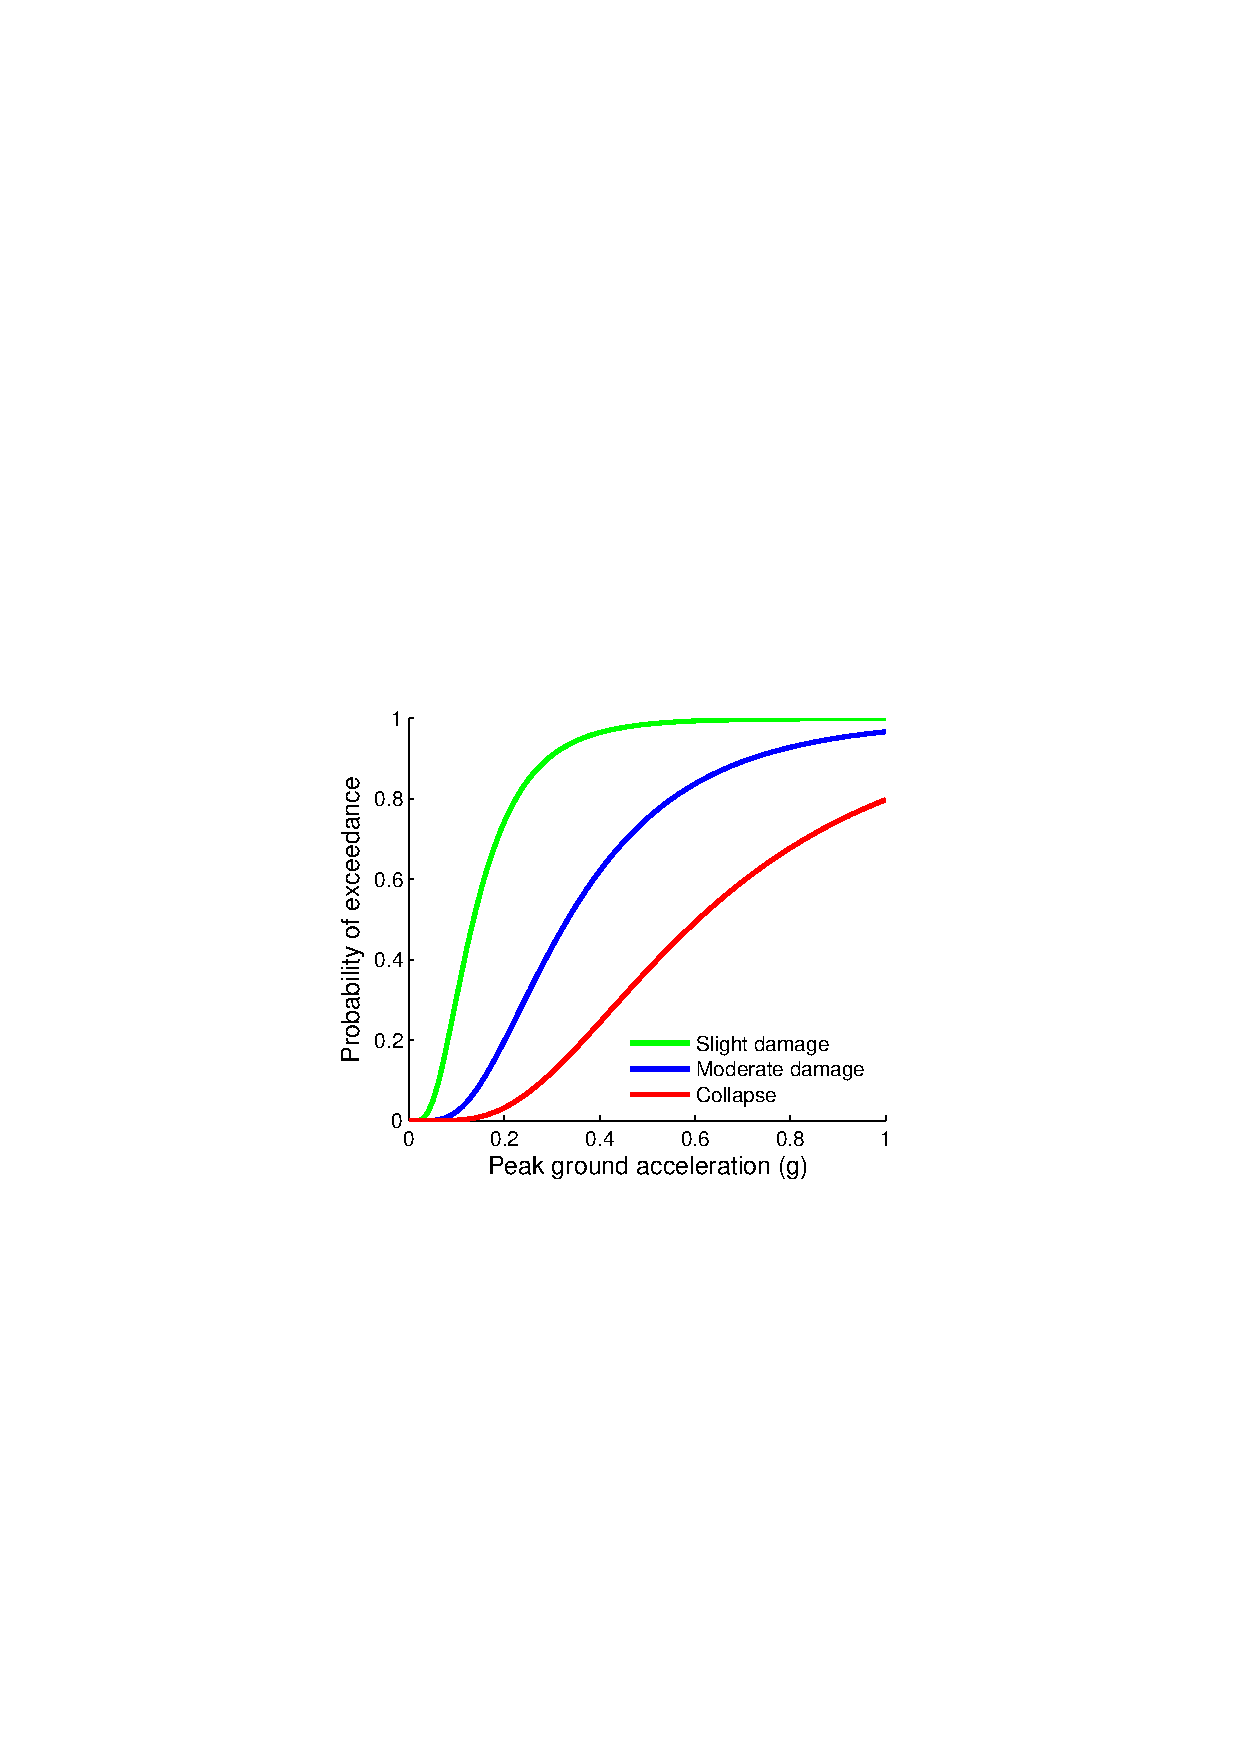
\includegraphics[width=8cm,height=6cm]{figures/risk/ConFragilityModel.pdf}
\caption{Graphical representation of a continuous fragility model.}
\label{fig:fragModelContinuous}
\end{figure}

The NRML schema to store these functions has an initial structure similar to that described for the discrete \glspl{fragility model}. Then, the continuous limit state curves are stored as illustrated below:

\begin{Verbatim}[frame=single, commandchars=\\\{\}, samepage=true]
    ...
    <\textcolor{green}{ffs noDamageLimit= 0.05}>
        <\textcolor{blue}{taxonomy} RC <\textcolor{blue}{/taxonomy}>
        <\textcolor{blue}{IML} IMT="PGA" minIML="0.0" maxIML="1.0" imlUnit="g" ><\textcolor{blue}{/IML}>
        <\textcolor{blue}{ffd} ls="slight">
            <params \textcolor{magenta}{mean}="0.16" \textcolor{magenta}{stddev}="0.11" />
        <\textcolor{blue}{/ffd}
        <\textcolor{blue}{ffd} ls="moderate">
            <params \textcolor{magenta}{mean}="0.40" \textcolor{magenta}{stddev}="0.26" />
        <\textcolor{blue}{/ffd}
        <\textcolor{blue}{ffd} ls="collapse">
            <params \textcolor{magenta}{mean}="0.73" \textcolor{magenta}{stddev}="0.48" />
        <\textcolor{blue}{/ffd}
    <\textcolor{green}{/ffs}>
<\textcolor{red}{/fragilityModel}>
</nrml>
\end{Verbatim}

Again, the set of limit state curves for each building typology needs to be stored within the field \Verb+ffs+ (fragility function set), through the definition of the following attributes:

\begin{itemize}
\item  \Verb+noDamageLimit+: this attribute defines the intensity measure level below which the probability of exceedance for all curves is zero;
\item  \Verb+type+: this parameter defines the type of probabilistic distribution being used to define the limit state curves. Currently the engine only supports lognormal distributions, however, the capability of considering other types of distributions (e.g. normal, exponential) will be developed in the future;
\item  \Verb+taxonomy+: a unique key that is used to relate each \gls{fragility function} with the relevant \glspl{asset} in the \gls{exposure model};
\item  \Verb+IML+: in this field, the intensity measure type (\Verb+IMT+) and associated units (\Verb+imlUnit+) for the limit state curves is defined, along with the minimum (\Verb+minIML+) and maximum (\Verb+maxIML+) intensity measure levels enclosing the range of applicability of the set of fragility functions;
\item  \Verb+ffc+: this field (fragility function continuous) is used to define the mean (\Verb+mean+) and standard deviation (\Verb+stddev+) of the cumulative lognormal function. In addition, the limit state for the curve being defined needs to be specified in the attribute \Verb+ls+.
\end{itemize}

\section{Consequence models}
\label{sec:consequence}
\input{oqum/risk/00c_consequence}

\section{Vulnerability models}
\label{sec:vulnerability}
In this section, the NRML schema for the \gls{vulnerability model} is
described in detail. In order to do so, a graphical representation of a
\gls{vulnerability model} (mean loss ratio for a set of intensity measure
levels) is illustrated in Figure~\ref{fig:vulModel}. Note that although the
uncertainty for each loss ratio is not represented in the aforementioned
figure, it can be considered in the input NRML file, by means of a coefficient
of variation per loss ratio and a probabilistic distribution, which can
currently be set to lognormal (LN) or Beta (BT).

\begin{figure}[ht]
\centering
\includegraphics[width=10cm,height=6cm]{figures/risk/vulnerabilityModel.pdf}
\caption{Graphical representation of a vulnerability model.}
\label{fig:vulModel}
\end{figure}

An example vulnerability model comprising three vulnerability functions is
shown below. This vulnerability model contains one function that uses the 
lognormal distribution to represent the uncertainty in the loss ratio at 
different intensity levels, one function that uses the Beta distribution, and
one function that is defined using a discrete probability mass distribution.

\inputminted[firstline=1,firstnumber=1,fontsize=\footnotesize,frame=single,linenos,bgcolor=lightgray]{xml}{oqum/risk/Verbatim/input_vulnerability.xml}\\


The initial portion of the schema contains general information that describes
some general aspects of the vulnerability model. The information in this
metadata section is common to all of the functions in the vulnerability model
and needs to be included at the beginning of every vulnerability model file.
The parameters are described below:

\begin{itemize}

    \item \Verb+id+: a unique key used to identify the \gls{vulnerability model}

    \item \Verb+assetCategory+: an optional string used to specify the type of
    \glspl{asset} for which vulnerability functions will be defined in this file 
    (e.g: buildings, lifelines)

    \item \Verb+lossCategory+: valid strings for this attribute are 
    ``structural'', ``nonstructural'', ``contents'',  
    ``business\_interruption'', and ``occupants''

    \item \Verb+description+: a brief string with further information about the
    \gls{vulnerability model}, for example, which building typologies are 
    covered or the source of the functions in the \gls{vulnerability model}

\end{itemize}

\inputminted[firstline=4,firstnumber=4,lastline=8,fontsize=\footnotesize,frame=single,linenos,bgcolor=lightgray]{xml}{oqum/risk/Verbatim/input_vulnerability.xml}\\


In order to perform probabilistic or scenario risk calculations, it is
necessary to define a vulnerability function for each building typology
present in the exposure model. The vulnerability functions require the user to
specify the distribution of the loss ratio for a set of intensity levels. The
loss ratio distributions can be defined using either a discrete or a
continuous format, and the fragility model file can include a mix of both
types of vulnerability functions. It is also possible to define a
vulnerability function using a set of deterministic loss ratios corresponding
to a set of intensity levels (i.e., ignoring the uncertainty in the
conditional loss ratios).

The following snippet from the above vulnerability model example file defines
a vulnerability function modelling the uncertainty in the conditional loss
ratios using a (continuous) lognormal distribution:

\inputminted[firstline=10,firstnumber=10,lastline=14,fontsize=\footnotesize,frame=single,linenos,bgcolor=lightgray]{xml}{oqum/risk/Verbatim/input_vulnerability.xml}\\

The following attributes are needed to define a vulnerability function which
uses a continuous distribution to model the uncertainty in the conditional
loss ratios:

\begin{itemize}

    \item \Verb+id+: a unique key used to identify the \gls{taxonomy} for 
    which the function is being defined. This key is used to relate the 
    \gls{vulnerability function} with the relevant \gls{asset} in the 
    \gls{exposure model}.

    \item \Verb+dist+: for vulnerability function which use a continuous 
    distribution to model the uncertainty in the conditional loss ratios, 
    this attribute should be set to either ``\Verb+LN+'' if using the lognormal
    distribution, or to ``\Verb+BT+'' if using the Beta distribution.

    \item \Verb+imls+: this attribute specifies the list of intensity levels
    for which the parameters of the conditional loss ratio distributions will
    be defined. In addition, it is also necessary to define the intensity 
    measure type (\Verb+imt+).

    \item \Verb+meanLRs+: this field is used to define the mean loss ratios
    for this \gls{vulnerability function} for each of the intensity levels
    defined by the attribute \Verb+imls+. The number of mean loss ratios
    defined by the \Verb+meanLRs+ attribute must be equal to the number of
    intensity levels defined by the attribute \Verb+imls+.

    \item \Verb+covLRs+: this field is used to define the coefficient of 
    variation for the conditional distribution of the loss ratios for this
    \gls{vulnerability function} for each of the intensity levels defined by
    the attribute \Verb+imls+. The number of coefficients of variation of loss
    ratios defined by the \Verb+covLRs+ attribute must be equal to the number
    of intensity levels defined by the attribute \Verb+imls+. The uncertainty
    in the conditional loss ratios can be ignored by setting all of the
    \Verb+covLRs+ for a given \gls{vulnerability function} to zero.

\end{itemize}

Several methodologies to derive vulnerability functions are currently being
evaluated by \gls{acr:gem} and have been included as part of the Risk
Modeller's Toolkit, the code for which can be found on a public repository at
GitHub at the following address
\href{http://github.com/gemsciencetools/rmtk}{http://github.com/gemsciencetools/rmtk}.

Scripts to convert \glspl{vulnerability function} in CSV format or as Excel or
ASCII files into NRML are also under development, and can be found at the
OpenQuake platform at the following address:
\href{https://platform.openquake.org/risk_input_preparation_toolkit/}{https://platform.openquake.org/risk\_input\_preparation\_toolkit/}.


\section{Calculation workflows}
\label{sec:risk_workflows}
\subsection{Scenario Damage Assessment}
\index{OpenQuake-engine!Risk calculation workflows!Scenario Damage Assessment}
\label{subsec:workflow_scenario_damage}
This calculator is capable of assessing the damage distribution due to a
single scenario earthquake, for a collection of assets. Similarly to the
previous calculator, in order to perform the necessary risk calculations one
or a set of ground motion fields are required, which can be derived using the
oq-hazardlib, or introduced in the OpenQuake-engine using the appropriate NRML
schema. In this calculator, a fragility model is combined with the
distribution of ground motion at the location of each asset, to estimate the
number or area of buildings in each damage state. The damage distribution can
be extracted per asset, per building typology (taxonomy) or considering all of
the assets simultaneously (total damage distribution). In addition, this
calculator also provides collapse maps, which contain the spatial distribution
of the number or area of collapsed buildings throughout the region of
interest. The input/output structure for this calculator is presented in
Figure~\ref{fig:io-structure-scenario-damage}.

\begin{figure}[ht]
\centering
\includegraphics[width=9cm,height=7cm]{figures/risk/io-structure-scenario-damage.pdf}
\caption{Scenario Damage Calculator input/output structure.}
\label{fig:io-structure-scenario-damage}
\end{figure}

\subsection{Scenario Risk Assessment}
\index{OpenQuake-engine!Risk calculation workflows!Scenario Risk Assessment}
\label{subsec:workflow_scenario_risk}
This calculator computes loss maps and loss statistics due to a single seismic
event, for a collection of assets. The hazard input can be a single ground
motion field (e.g. the median distribution of ground motion in the region of
interest) or a set of ground motion fields allowing the characterisation of
the inter- and intra-event variability from the GMPE. It is noted that the
hazard input can either be calculated using the hazard component of OpenQuake-
engine (oq-hazardlib), or provided to the risk component iian external file
following the respective Natural hazards' Risk Markup Language (NRML) schema
(see \href{http://github.com/gem/oq-nrmllib}{oq-nrmllib}). A vulnerability
model is combined with the distribution of the ground motions at each asset
location to calculate the loss distribution for each asset, as well as the
statistics of the total loss throughout the region of interest. The required
input files and resulting output files are depicted in
Figure~\ref{fig:io-structure-scenario-risk}.

\begin{figure}[ht]
\centering
\includegraphics[width=9cm,height=7cm]{figures/risk/io-structure-scenario-risk.pdf}
\caption{Scenario Risk Calculator input/output structure.}
\label{fig:io-structure-scenario-risk}
\end{figure}

\subsection{Classical Probabilistic Seismic Damage Analysis}
\index{OpenQuake-engine!Risk calculation workflows!Classical Probabilistic Seismic Damage Analysis}
\label{subsec:workflow_classical_damage}
The classical PSHA-based damage calculator convolves through numerical integration, the damage state fragility functions for an asset with the seismic hazard curve at the location of the asset. The main results of this calculator are damage distribution statistics for each asset, which describe the expected fraction of buildings in each damage state. Furthermore, a probabilistic collapse map can be extracted giving the probability of collapse for each asset within the specified time period. Damage distribution aggregated by taxonomy or of the total portfolio (considering all assets in the exposure model) can not be extracted using this calculator, as the spatial correlation of the ground motion residuals is not taken into consideration. The input and output files involved in this calculator are presented in Figure~\ref{fig:ClassicalDamage}.

\begin{figure}[ht]
\centering
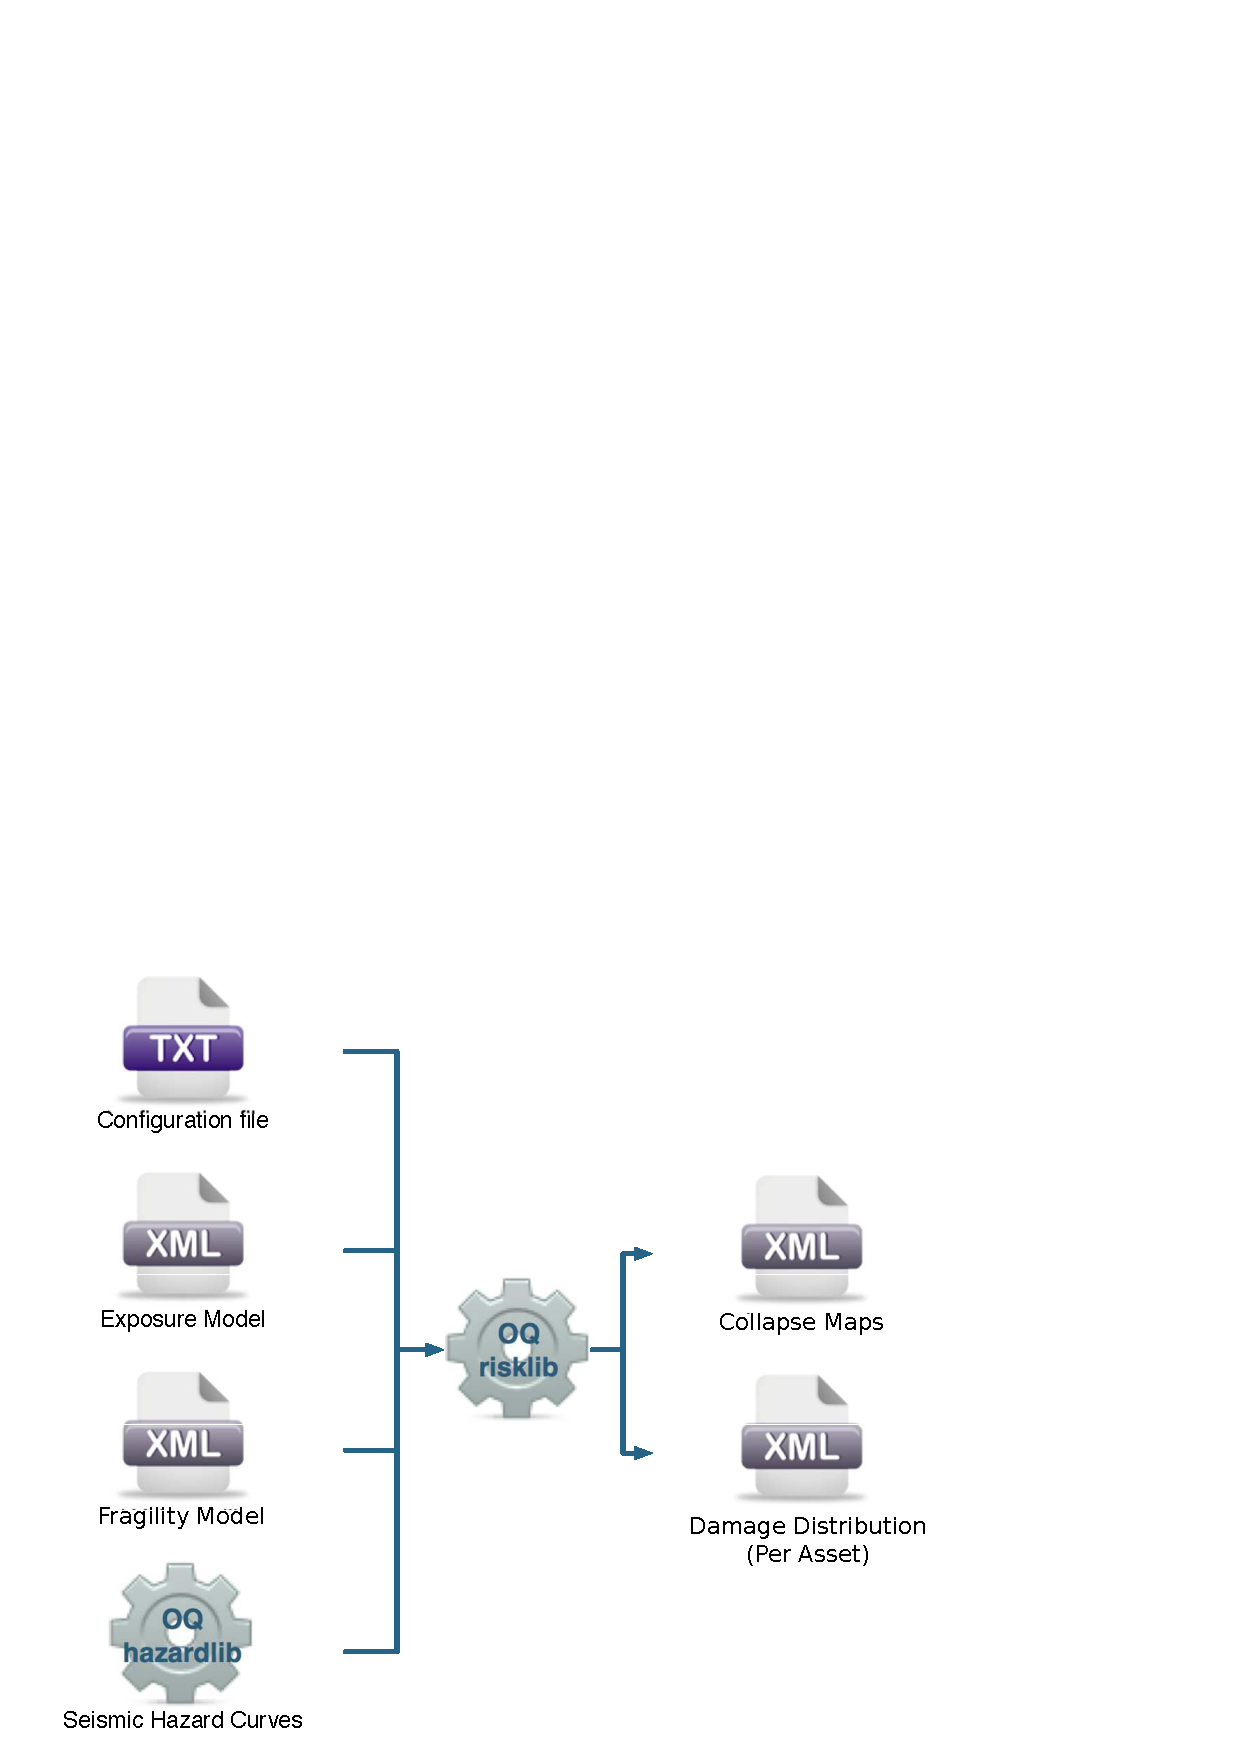
\includegraphics[width=9cm,height=7cm]{figures/risk/ClassicalDamage.pdf}
\caption{Classical PSHA-based Damage Calculator input/output structure.}
\label{fig:ClassicalDamage}
\end{figure}

\subsection{Classical Probabilistic Seismic Risk Analysis}
\index{OpenQuake-engine!Risk calculation workflows!Classical Probabilistic Seismic Risk Analysis}
\label{subsec:workflow_classical_risk}
In this calculator, probabilistic seismic hazard is employed to calculate a loss exceedance curve for each asset, through the usage of seismic hazard curves. A convolution between the vulnerability function and the hazard curve at location of the asset is performed, leading to the probability of exceeding a set of loss ratios. Each loss ratio is multiplied by the asset value to obtain the final loss exceedance curve. Furthermore, probabilistic loss maps can be extracted by interpolating the loss curves at each location by various probabilities of exceedance. Unlike what was described in the previous calculator, a total loss curve (considering all assets in the exposure model) can not be extracted using this calculator, as the correlation of the ground motion residuals and vulnerability uncertainty is not taken into consideration. The input and output files involved in this calculator are presented in Figure~\ref{fig:ClassicalRisk}.

\begin{figure}[ht]
\centering
\includegraphics[width=9cm,height=7cm]{figures/risk/ClassicalRisk.pdf}
\caption{Classical PSHA-based Risk Calculator input/output structure.}
\label{fig:ClassicalRisk}
\end{figure}

\subsection{Event-Based Probabilistic Seismic Risk Analysis}
\index{OpenQuake-engine!Risk calculation workflows!Event-Based Probabilistic Seismic Risk Analysis}
\label{subsec:workflow_event_based_risk}
In this calculator, loss exceedance curves and loss maps for various return
periods can be calculated, based on probabilistic seismic hazard, with an
event-based approach. A large number of stochastic event sets are generated,
and the associated ground motion fields for each event are used together with
a vulnerability model to compute the individual (per asset) and total (sum of
all the losses per event) losses. Then, this distribution of losses is
employed to derive a loss exceedance curve per asset, as well as a total loss
exceedance curve representative of the complete building portfolio.
Furthermore, oq-risklib can also compute loss maps for various return periods
by interpolating each individual loss curve with the respective probability of
exceedance. In Figure~\ref{fig:io-structure-event-based-risk}, the
input/output scheme of this calculator is illustrated.

\begin{figure}[ht]
\centering
\includegraphics[width=9cm,height=7cm]{figures/risk/io-structure-event-based-risk.pdf}
\caption{Probabilistic Event-based Risk Calculator input/output structure.}
\label{fig:io-structure-event-based-risk}
\end{figure}

\subsection{Retrofit Benefit-Cost Ratio Analysis}
\index{OpenQuake-engine!Risk calculation workflows!Retrofit Benefit-Cost Ratio Analysis}
\label{subsec:workflow_benefit_cost}
\input{oqum/risk/00e_workflow_benefit_cost}

\cleardoublepage
   \cleardoublepage

\chapterimage{figures/chapter_head_2.pdf} % Chapter heading image
\chapter{Using the Risk Module}
	\label{chap:riskinputs}
	This Chapter summarises the structure of the information necessary to define
the different input data to be used with the OpenQuake-engine risk 
calculators.

Input data for scenario-based and probabilistic seismic damage and risk
analysis using OpenQuake-engine are organised into:

\begin{itemize}

  \item A general calculation configuration file.

  \item A file describing the exposure model.

  \item A file describing the vulnerability model for loss calculations, or a 
  		file describing the fragility model for damage calculations. Optionally, 
  		a file describing the consequence model can also be provided in order 
  		to calculate losses from the estimated damage distributions.

  \item Hazard inputs

\end{itemize}

% Figure~\ref{fig:risk_input} summarises the structure of a risk input model
% for the OpenQuake-engine and the relationships between the different files.

% \begin{figure}[!ht]
% \centering
% \includegraphics[width=14cm]{figures/risk/risk_input_structure.pdf}
% \caption{PSHA Input Model structure}
% \label{fig:risk_input}
% \end{figure}

% \section{Defining Logic Trees}
% The main components of a logic tree structure in the OpenQuake engine are 
the following:
\begin{description}
    \item[branch]: the simplest component of a logic tree structure. 
    A branch represent an alternative 
    \item[branching set]: it groups a set of branches i.e. 
    alternative interpretation of a parameter or a model. This set of 
    uncertainties can be applied to the whole initial seismic source input 
    model or to a subset of seismic source data. The sum of the 
    weights/probabilities assigned to the set of branches 
    \item[branching level]: it's the largest container. It's not used in 
    modelling uncertainty, but it's useful in maintaining a logic and an 
    order in the structure of the logic tree as it's will be explained in 
    the following examples.
\end{description}

% \label{sec:risk_logic_trees}

\section{Configuration file}
\index{Input!Configuration file}
\label{sec:risk_configuration_file}
The configuration file (or job.ini file) represents the location where the
paths to the input files, the parameters controlling the risk calculations and
the type of outputs are defined. Some initial parameters common to all the
risk calculators are presented below. The remaining parameters that are
specific to each risk calculator are discussed in subsequent sections. For
additional information about how each parameter is being used within the
methodologies implemented in the oq-engine, users advised to consult the
OpenQuake-engine Book (Risk).

\begin{Verbatim}[frame=single, commandchars=\\\{\}, samepage=true]
[general]
description = Scenario Risk Nepal
calculation_mode = scenario_risk

exposure_file = exposure_model.xml
region_constraint = 78.0 31.5,89.5 31.5,89.5 25.5,78 25.5
asset_hazard_distance = 10
...
\end{Verbatim}

\begin{itemize}
\item  \Verb+description+: a parameter that can be used to include some information about the type of calculations that are going to be performed;
\item  \Verb+calculation_mode+: this parameter sets the type of calculations. The key word for each risk calculator is described in the following sections;
\item  \Verb+exposure_file+: this parameter is used to specify the path to the \gls{exposure model} file;
\item  \Verb+region_constraint+: this field is used to define the polygon enclosing the region of interest. Assets outside of this region will not be considered in the risk calculations. This region is defined using pairs of coordinates (longitude and latitude in decimal degrees) that indicate the vertices of the polygon;
\item  \Verb+asset_hazard_distance+: this parameter indicates the maximum allowable distance between an \gls{asset} and the closest hazard input. If no hazard input is found within this distance, the \gls{asset} is skipped and a message is provided mentioning the id of the asset that is affected by this issue. If this parameter is not provided, the OpenQuake-Engine assumes the maximum allowable distance as 5 km.
\end{itemize}

Depending on the type of calculations, other parameters besides the
aforementioned ones need to be provided, as will be described in the following
sections.

\subsection{Scenario Damage Calculator}
\label{subsec:config_scenario_damage}
For this calculator, the parameter \Verb+calculation_mode+ needs to be defined as \Verb+scenario_damage+. There is only one parameter specific to this calculator, which is the \gls{fragility model} file path, as presented below.

\begin{Verbatim}[frame=single, commandchars=\\\{\}, samepage=true]
...
fragility_file = fragility_model.xml
\end{Verbatim}

\begin{itemize}
\item  \Verb+fragility_file+: a parameter used to define the path to the \gls{fragility model} file.
\end{itemize}

\subsection{Scenario Risk Calculator}
\label{subsec:config_scenario_risk}
In order to run this calculator, the parameter \Verb+calculation_mode+ needs to be set to \Verb+scenario_risk+. The remaining parameters are illustrated bellow.

\begin{Verbatim}[frame=single, commandchars=\\\{\}, samepage=true]
...
structural_vulnerability_file = struct_vul_model.xml
nonstructural_vulnerability_file = nonstruct_vul_model.xml
contents_vulnerability_file = cont_vul_model.xml
business_interruption_vulnerability_file = bus_int_vul_model.xml
occupants_vulnerability_file = occ_vul_model.xml

asset_correlation = 0.7
master_seed = 3
insured_losses = true
\end{Verbatim}

\begin{itemize}
\item  \Verb+structural_vulnerability_file+: this parameter is used to specify the path to the structural \gls{vulnerability model} file;
\item  \Verb+nonstructural_vulnerability_file+: this parameter is used to specify the path to the non-structural\gls{vulnerability model} file;
\item  \Verb+contents_vulnerability_file +: this parameter is used to specify the path to the contents \gls{vulnerability model} file;
\item  \Verb+business_interruption_vulnerability_file +: this parameter is used to specify the path to the business interruption \gls{vulnerability model} file;
\item  \Verb+vulnerability_file+: this parameter is used to specify the path to the occupants \gls{vulnerability model} file;
\item \texttt{asset\_cor\-re\-la\-tion} if the uncertainty in the loss ratios has been defined within the \gls{vulnerability model}, users can specify a coefficient of correlation that will be used in the Monte Carlo sampling process of the loss ratios, between the assets that share the same \gls{taxonomy}. If the \texttt{asset\_cor\-re\-la\-tion} is set to one, the loss ratio residuals will be perfectly correlated. On the other hand, if this parameter is set to zero, the loss ratios will be sampled independently. Any value between zero and one will lead to increasing levels of correlation. If this parameter is not defined, the OpenQuake-engine assumes no correlation in the vulnerability;
\item  \Verb+master_seed+: this parameter is used to control the random generator in the loss ratio sampling process. This way, if the same \Verb+master_seed+ is defined at each calculation run, the same random loss ratios will be generated, thus allowing replicability of the results;
\item  \Verb+insured_losses+: this parameter is used to define if insured losses should be calculated (\Verb+true+) or not (\Verb+false+).
\end{itemize}

\subsection{Classical Probabilistic Seismic Damage Calculator}
\label{subsec:config_classical_damage}
\input{oqum/risk/01a_config_classical_damage}

\subsection{Classical Probabilistic Seismic Risk Calculator}
\label{subsec:config_classical_risk}
\input{oqum/risk/01a_config_classical_risk}

\subsection{Event-Based Probabilistic Seismic Risk Calculator}
\label{subsec:config_event_based_risk}
\input{oqum/risk/01a_config_event_based_risk}

\subsection{Retrofit Benefit-Cost Ratio Calculator}
\label{subsec:config_benefit_cost}
\input{oqum/risk/01a_config_benefit_cost}

\cleardoublepage
   \cleardoublepage

\chapterimage{figures/chapter_head_2.pdf} % Chapter heading image
\chapter{Risk Calculations and Results}
	\label{chap:riskoutputs}
	In this Chapter we provide a desciption of the main commands available for
running hazard with the \gls{acr:oqe} and the file formats used to represent
the results of the analyses.

A general introduction on the use of the \glsdesc{acr:oqe} is provided in
Section~\ref{sec:running_oq_engine} at page~\pageref{sec:running_oq_engine}. The
reader is invited to consult this part before diving into the following
sections.


% -----------------------------------------------------------------------------
\section{Running OpenQuake-engine for hazard calculations}
\label{sec:running_hazard_calculations}
\index{Running OpenQuake!hazard}

The execution of a hazard analysis using the OpenQuake-engine is
straightforward. Below we provide an example of the simplest command that can be
used to launch a hazard calculation. It consists in the invocation of \texttt
{oq-engine} together with the \texttt{--rh} option which stands for ``run
hazard'' and the name of a configuration file (in the example below it
corresponds to \texttt{job.ini}):

\begin{Verbatim}[frame=single, commandchars=\\\{\}, fontsize=\small]
user@ubuntu:~$ oq-engine --rh job.ini
\end{Verbatim}

The amount of information prompted during the execution of the analysis can be
controlled through the \texttt{--log-level} flag as shown in the example below:

\begin{Verbatim}[frame=single, commandchars=\\\{\}, fontsize=\small]
user@ubuntu:~$ oq-engine --rh job.ini --log-level debug
\end{Verbatim}

In this example we ask the engine to provide an extensive amount of information
(usually not justified for a standard analysis). Alternative options are:
\texttt{debug}, \texttt{info}, \texttt{progress}, \texttt{warn}, \texttt{error},
\texttt{critical}.


% -----------------------------------------------------------------------------
\section{Exporting results from a hazard calculation}
\label{sec:exporting_hazard_results}

There are two alternative ways to get results from the OpenQuake-engine:
directly through the calculation or by exporting them from the internal
\gls{acr:oqe} database once a calculation is completed.

The first option is defined at the OpenQuake-engine invocation through the
flag \texttt{--exports xml}, as shown in the example below:

\begin{Verbatim}[frame=single, commandchars=\\\{\}, fontsize=\small]
user@ubuntu:~$ oq-engine --rh job.ini \textcolor{red}{--exports xml}
\end{Verbatim}

The second option allows the user to export the computed results or just a
subset of them whenever they want. In order to obtain the list of results of
the hazard calculations stored in the \gls{acr:oqe} database the user can
utilize the following command:

\begin{Verbatim}[frame=single, commandchars=\\\{\}, fontsize=\small]
user@ubuntu:~$ oq-engine --lhc
\end{Verbatim}

The execution of this command will produce a list similar to the one provided
below (the numbers in red are the calculations IDs):

\begin{Verbatim}[frame=single, commandchars=\\\{\}, fontsize=\small]
user@ubuntu:~$ oq-engine --lhc
calc_id | num_jobs | latest_job_status | last_update | description
\textcolor{red}{1} | 1 | failed | 2013-03-01 09:49:34 | Classical PSHA
\textcolor{red}{2} | 1 | successful | 2013-03-01 09:49:56 | Classical PSHA
\textcolor{red}{3} | 1 | failed | 2013-03-01 10:24:04 | Classical PSHA
\textcolor{red}{4} | 1 | failed | 2013-03-01 10:28:16 | Classical PSHA
\textcolor{red}{5} | 1 | failed | 2013-03-01 10:30:04 | Classical PSHA
\textcolor{red}{6} | 1 | successful | 2013-03-01 10:31:53 | Classical PSHA
\textcolor{red}{7} | 1 | failed | 2013-03-09 08:15:14 | Classical PSHA
\textcolor{red}{8} | 1 | successful | 2013-03-09 08:18:04 | Classical PSHA
\end{Verbatim}

Subsequently the user can get the list of result stored for a specific hazard
analysis as in the example below (note that the number in blue emphasizes the
result ID):

\begin{Verbatim}[frame=single, commandchars=\\\{\}, fontsize=\small]
user@ubuntu:~$ oq-engine --lho <calc_id>
id | output_type | name
\textcolor{blue}{3} | hazard_curve | hc-rlz-6
\end{Verbatim}

and finally extract an xml file for a specific hazard result:

\begin{Verbatim}[frame=single, commandchars=\\\{\}, fontsize=\small]
user@ubuntu:~$ oq-engine --eh <result_id> <path_to_the_output_folder>
\end{Verbatim}


% -----------------------------------------------------------------------------
\section{Description of hazard outputs}
\label{sec:hazard_outputs}

The results generated by the OpenQuake-engine are fundamentally of two
distinct typologies differentiated by the presence (or absence) of epistemic
uncertainty in the PSHA input model.

When epistemic uncertainty is incorporated into the calculation, the
OpenQuake-engine calculators (e.g. Classical PSHA, Event Based PSHA,
Disaggregation, UHS) produce a set of results (i.e. hazard curves, ground
motion fields, disaggregation matrices, UHS, for each logic-tree realisation)
which reflects epistemic uncertainties introduced in the PSHA input model.

For each logic tree sample, results are computed and stored. Calculation of
results statistics (mean, standard deviation, quantiles) are supported by all
the calculators, with the exception of the disaggregation calculator.

\subsection{Outputs from Classical PSHA}
\label{subsec:output_classical_psha}
By default, the classical PSHA calculator computes and stores hazard curves
for each logic tree sample considered.

When the PSHA input model doesn't contain epistemic uncertainties the results
is a set of hazard curves (one for each investigated site). The command below
illustrates how is possible to retrieve the group of hazard curves obtained
for a calculation with a given identifier \texttt{<calc\_id>} (see
Section~\ref{sec:exporting_hazard_results} for an explanation about how to
obtain the list of calculations performed with their corresponding ID):

\begin{Verbatim}[frame=single, commandchars=\\\{\}, fontsize=\small]
user@ubuntu:~$ oq engine --lo <calc_id>
id | output_type | name
\textcolor{red}{3 | datastore | hcurves}
4  | datastore | realizations
\end{Verbatim}

%The user need not concern them-self with the realizations output. 
%
%In this case the \gls{acr:oqe} computed a group of hazard curves with result
%ID equal to \texttt{3}. On the contrary, if the parameter
%\texttt{number\_of\_logic\_tree\_samples} in the configuration file is
%different than zero, then N hazard curves files are generated. The example
%below shows this case:
%
%\begin{Verbatim}[frame=single, commandchars=\\\{\}, fontsize=\small]
user@ubuntu:~$ oq-engine --lho <calc_id>
id | output_type | name
\textcolor{red}{5 | hazard_curve | hc-rlz-10}
\textcolor{red}{6 | hazard_curve | hc-rlz-7}
\textcolor{red}{7 | hazard_curve | hc-rlz-8}
\textcolor{red}{8 | hazard_curve | hc-rlz-9}
\textcolor{red}{9 | hazard_curve | hc-rlz-11}
\textcolor{red}{10 | hazard_curve | hc-rlz-12}
\end{Verbatim}


To export from the database the outputs (in this case hazard curves)  contained in one of the output identifies, one can do so with the following command:

\begin{Verbatim}[frame=single, commandchars=\\\{\}, fontsize=\small]
user@ubuntu:~$ oq engine --export-output <output_id> <output_directory>
\end{Verbatim}

Alternatively, if the user wishes to export all of the outputs associated with a particular calculation then they can use the \texttt{-{}-export-outputs} with the corresponding calculation key:

\begin{Verbatim}[frame=single, commandchars=\\\{\}, fontsize=\small]
user@ubuntu:~$ oq engine --export-outputs <calc_id> <output_directory>
\end{Verbatim}

The exports will produce one or more nrml files containing the seismic hazard curves, as represented in the example in the inset
below:

\input{oqum/hazard/verbatim/output_hazard_curves}

Notwithstanding the intuitiveness of this file, let's have a brief
overview of the information included.

The overall content of this file is a list of hazard curves, one for each
investigated site, computed using a PSHA input model representing one possible
realisation obtained using the complete logic tree structure.

The attributes of the \texttt{hazardCurves} element (see text in red) specify
the path of the logic tree used to create the seismic source model
(\texttt{source\-Model\-TreePath}) and the ground motion model
(\texttt{gsim\-Tree\-Path}) plus the intensity measure type and the
investigation time used to compute the probability of exceedance.

The \texttt{IMLs} element (in green in the example) contains the values of
shaking used by the engine to compute the probability of exceedance in the
investigation time. For each site this file contains a \texttt{hazardCurve}
element which has the coordinates (longitude and latitude in decimal degrees)
of the site and the values of the probability of exceedance for all the
intensity measure levels specified in the \texttt{IMLs} element.

If the hazard calculation is configured to produce results including seismic hazard maps and uniform hazard spectra, then the list of outputs would display the following:

\begin{Verbatim}[frame=single, commandchars=\\\{\}, fontsize=\small]
user@ubuntu:~$ oq engine --lo <calc_id>
id | output_type | name
\textcolor{red}{3 | datastore | hcurves}
\textcolor{red}{4 | datastore | hmaps}
5  | datastore | realizations
\textcolor{red}{6 | datastore | uhs}
\end{Verbatim}

%\input{oqum/hazard/verbatim/output_classical_multiple_rlz}

%In this example the \gls{acr:oqe} produced hazard curves and hazard maps for
%six logic tree realisations plus median hazard curves and the median hazard
%map (both highlighted in red).

The following inset shows a sample of the nrml file used to describe a hazard map:

\input{oqum/hazard/verbatim/output_hazard_map}

\noindent and a uniform hazard spectrum:

\input{oqum/hazard/verbatim/output_uhs}

\subsection{Outputs from Hazard Disaggregation}
\label{subsec:output_hazard_disaggregation}
\section{Output from Disaggregation}
The \gls{acr:oqe} output of a disaggregation analysis  
corresponds to the combination of a hazard curve and a multidimensional 
matrix containing the results of the disaggregation.

The example below shows the list of disaggregation results obtained 
for four logic tree realisations. 
%
For each realisation, disaggregation has been completed for two  
intensity measure levels corresponding to different probabilities of 
exceedence in the specified \texttt{investigation time}.
\begin{Verbatim}[frame=single, commandchars=\\\{\}]
user@ubuntu:~$ openquake --lho <calc_id> 
id | output_type | name
19 | hazard_curve | hc-rlz-3
20 | hazard_curve | hc-rlz-3
21 | hazard_curve | hc-rlz-4
22 | hazard_curve | hc-rlz-4
23 | disagg_matrix | disagg(0.02)-rlz-3-SA(0.025)-POINT(10.1 40.1)
24 | disagg_matrix | disagg(0.1)-rlz-3-SA(0.025)-POINT(10.1 40.1)
25 | disagg_matrix | disagg(0.02)-rlz-3-PGA-POINT(10.1 40.1)
26 | disagg_matrix | disagg(0.1)-rlz-3-PGA-POINT(10.1 40.1)
27 | disagg_matrix | disagg(0.02)-rlz-4-SA(0.025)-POINT(10.1 40.1)
28 | disagg_matrix | disagg(0.1)-rlz-4-SA(0.025)-POINT(10.1 40.1)
29 | disagg_matrix | disagg(0.02)-rlz-4-PGA-POINT(10.1 40.1)
30 | disagg_matrix | disagg(0.1)-rlz-4-PGA-POINT(10.1 40.1)
\end{Verbatim}

In the following inset we show an example of the nrml file 
used to represent the different disaggregation matrices (highlighted 
in red) produced by OpenQuake-engine.
%
\begin{Verbatim}[frame=single, commandchars=\\\{\}, fontsize=\small]
<?xml version='2.0' encoding='UTF-8'?>
<nrml xmlns:gml="http://www.opengis.net/gml" 
      xmlns="http://openquake.org/xmlns/nrml/0.4">
  <disaggMatrices sourceModelTreePath="b1" gsimTreePath="b1" IMT="PGA" 
        investigationTime="50.0" lon="10.1" lat="40.1" 
        magBinEdges="5.0, 6.0, 7.0, 8.0" 
        distBinEdges="0.0, 25.0, 50.0, 75.0, 100.0" 
        lonBinEdges="9.0, 10.5, 12.0" 
        latBinEdges="39.0, 40.5" 
        epsBinEdges="-3.0, -1.0, 1.0, 3.0" 
        tectonicRegionTypes="Active Shallow Crust">
\textcolor{red}{    <disaggMatrix type="Mag" dims="3" poE="0.1" }
\textcolor{red}{            iml="0.033424622602">}
      <prob index="0" value="0.987374744394"/>
      <prob index="1" value="0.704295394366"/>
      <prob index="2" value="0.0802318409498"/>
\textcolor{red}{    </disaggMatrix>}
\textcolor{red}{    <disaggMatrix type="Dist" dims="4" poE="0.1" }
\textcolor{red}{            iml="0.033424622602">}
      <prob index="0" value="0.700851969171"/>
      <prob index="1" value="0.936680387051"/>
      <prob index="2" value="0.761883595568"/>
      <prob index="3" value="0.238687565571"/>
\textcolor{red}{    </disaggMatrix>}
\textcolor{red}{    <disaggMatrix type="TRT" dims="1" poE="0.1" }
\textcolor{red}{            iml="0.033424622602">}
      <prob index="0" value="0.996566187011"/>
\textcolor{red}{    </disaggMatrix>}
\textcolor{red}{    <disaggMatrix type="Mag,Dist" dims="3,4" poE="0.1" }
\textcolor{red}{            iml="0.033424622602">}
      <prob index="2,3" value="0.0"/>
\textcolor{red}{    </disaggMatrix>}
\textcolor{red}{    <disaggMatrix type="Mag,Dist,Eps" dims="3,4,3" poE="0.1" }
\textcolor{red}{            iml="0.033424622602">}
      <prob index="0,0,0" value="0.0785857271425"/>
      ...
\textcolor{red}{    </disaggMatrix>}
\textcolor{red}{    <disaggMatrix type="Lon,Lat" dims="2,1" poE="0.1"}
\textcolor{red}{            iml="0.033424622602">}
      <prob index="0,0" value="0.996566187011"/>
      <prob index="1,0" value="0.0"/>
\textcolor{red}{    </disaggMatrix>}
\textcolor{red}{    <disaggMatrix type="Mag,Lon,Lat" dims="3,2,1" poE="0.1"} 
\textcolor{red}{            iml="0.033424622602">}
      <prob index="0,0,0" value="0.987374744394"/>
      <prob index="0,1,0" value="0.0"/>
      <prob index="1,0,0" value="0.704295394366"/>
      <prob index="1,1,0" value="0.0"/>
      <prob index="2,0,0" value="0.0802318409498"/>
      <prob index="2,1,0" value="0.0"/>
\textcolor{red}{    </disaggMatrix>}
\textcolor{red}{    <disaggMatrix type="Lon,Lat,TRT" dims="2,1,1" poE="0.1"} 
\textcolor{red}{            iml="0.033424622602">}
      <prob index="0,0,0" value="0.996566187011"/>
      <prob index="1,0,0" value="0.0"/>
\textcolor{red}{    </disaggMatrix>}
  </disaggMatrices>
</nrml>

\end{Verbatim}
%\caption{Hazard map: nrml sample file}
%\label{vrb:disaggr}
%\end{nrmlsmp}



\subsection{Outputs from Event Based PSHA}
\label{subsec:output_event_based_psha}
The Event Based PSHA calculator computes and stores stochastic event sets and
the corresponding ground motion fields.

This calculator can also produce hazard curves and hazard maps exactly in the
same way as done using the Classical PSHA calculator.

The inset below shows an example of the list of results provided by the
\gls{acr:oqe} at the end of an event-based PSHA calculation:

\begin{Verbatim}[frame=single, commandchars=\\\{\}, fontsize=\small]
user@ubuntu:~$ oq-engine --lho <calc_id>
id | output_type | name
\textcolor{red}{31 | ses | ses-coll-rlz-19}
\textcolor{green}{32 | gmf | gmf-rlz-19}
\textcolor{red}{33 | ses | ses-coll-rlz-20}
\textcolor{green}{34 | gmf | gmf-rlz-20}
35 | hazard_curve | hazard-curve-rlz-19-SA(0.1)
36 | hazard_curve | hazard-curve-rlz-20-SA(0.1)
37 | hazard_curve | hazard-curve-rlz-19-PGA
38 | hazard_curve | hazard-curve-rlz-20-PGA
39 | hazard_curve | mean curve for SA(0.1)
40 | hazard_curve | quantile curve (poe >= 0.15) for imt SA(0.1)
41 | hazard_curve | quantile curve (poe >= 0.50) for imt SA(0.1)
42 | hazard_curve | quantile curve (poe >= 0.85) for imt SA(0.1)
43 | hazard_curve | mean curve for PGA
44 | hazard_curve | quantile curve (poe >= 0.15) for imt PGA
45 | hazard_curve | quantile curve (poe >= 0.50) for imt PGA
46 | hazard_curve | quantile curve (poe >= 0.85) for imt PGA
\end{Verbatim}

This list in the inset above contains two sets of stochastic events (in red)
and two sets of ground motion fields (in blue).

The whole group of stochastic event set and ground motion fields can be
exported immediately using the results with \texttt{id} 35 and 25, respectively.

Below is an example showing a nrml file containing a collection of stochastic
event sets (2 ruptures):

\input{oqum/hazard/verbatim/output_ses}

The text in red shows the part which describes the id of the generated
stochastic event set and the investigation time covered.

The text in green emphasises the portion of the text used to describe a
rupture. The information provided describes entirely the geometry of the rupture as well as its rupturing properties (e.g. rake, magnitude). The rupture ID is a string that represents each rupture uniquely (including the case where the same rupture is sampled multiple times). The exact format may be subject to change from time-to-time; however, the ID will usually contain information regarding the specific logic tree branch sample (realisation), the stochastic event set counter, the ID of the source from which the rupture was samples and a unique number indicating the rupture identifier within the earthquake rupture forecast of the specific source.

This is an example of a nrml file containing one ground motion field:

\input{oqum/hazard/verbatim/output_gmf}


   \cleardoublepage

\chapterimage{figures/chapter_head_2.pdf} % Chapter heading image
\chapter{Demonstrative Examples}
	\label{chap:riskdemos}
	This sections describes the set of demos that have been compile to exercise the OpenQuake-engine. These demos can be found in a public repository in GitHub at the following link \href{http://github.com/gem/oq-engine/tree/master/demos}{http://github.com/gem/oq-engine/tree/master/demos}. Furthermore, a folder containing all of these demonstrative examples is provided when an OATS (OpenQuake Alpha Testing Service) account is requested, and it is also part of the OpenQuake-engine virtual image package. These examples are purely demonstrative and do not intend to represent accurately the seismicity, vulnerability or exposure characteristics of the region of interest, but simply to provide example input files that can be used as a benchmark for users planning to employ the OpenQuake-engine in seismic risk and loss estimation studies. Is is also noted that in the demonstrative examples presented in this section, illustrations about the various messages from the engine displayed in the command line interface are presented. These messages often contain information about the calculation id and output id, which will certainly be different for each user.

The five demos use Nepal as the region of interest. An example \gls{exposure model} has been developed for this region, comprising 9144 assets distributed amongst 2221 locations (due to the existence of more than one \gls{asset} at the same location). A map with the distribution of the number of buildings throughout Nepal is presented in Figure~\ref{fig:expNepal}.

\begin{figure}[ht]
\centering
\includegraphics[width=12cm,height=8cm]{figures/risk/NepalExposure.pdf}
\caption{Distribution of number of buildings in Nepal.}
\label{fig:expNepal}
\end{figure}

The building portfolio was organised into four classes for the rural areas (adobe, dressed stone, unreinforced fired brick, wooden frames), and five classes for the urban areas (the aforementioned typologies, in addition to reinforced concrete buildings). For each one of these building typologies, \glspl{vulnerability function} and \glspl{fragility function} were collected from the literature. These input models are only for demonstrative purposes and for further information about the building characteristics of Nepal, users are advised to contact the National Society for Earthquake Technology of Nepal (NSET - \href{http://www.nset.org.np/}{http:www.nset.org.np/}).

This section includes instructions not only on how to run the risk calculations, but also on how to produce the necessary hazard input. Thus, each demo comprises the configuration file, exposure model and fragility/vulnerability models fundamental for the risk calculations, but also a configuration file and associated input models to produce the hazard input.


\subsection{Scenario Damage Demos}
\label{subsec:demos_scenario_damage}
\input{oqum/risk/03a_demos_scenario_damage}

\subsection{Scenario Risk Demos}
\label{subsec:demos_scenario_risk}
\input{oqum/risk/03a_demos_scenario_risk}

\subsection{Classical Probabilistic Seismic Damage Demos}
\label{subsec:demos_classical_damage}
\input{oqum/risk/03a_demos_classical_damage}

\subsection{Classical Probabilistic Seismic Risk Demos}
\label{subsec:demos_classical_risk}
\input{oqum/risk/03a_demos_classical_risk}

\subsection{Event-Based Probabilistic Seismic Risk Demos}
\label{subsec:demos_event_based_risk}
\input{oqum/risk/03a_demos_event_based_risk}

\subsection{Retrofit Benefit-Cost Ratio Demos}
\label{subsec:demos_benefit_cost}
The loss exceedance curves used within this demo are produced using the Classical PSHA-based Risk calculator. Thus, the process to produce the seismic hazard curves described in the respective section (\ref{subsec:demos_classical_risk}) can be employed here. Then, the risk calculations can be initiated using the following command:

\begin{Verbatim}[frame=single, commandchars=\\\{\}, samepage=true]
user@ubuntu:~\$ oq-engine --rr job_bcr.ini --hazard-output-id 27
\end{Verbatim}

which should produce the following output:

\begin{Verbatim}[frame=single, commandchars=\\\{\}, samepage=true]
Calculation 17 results:
id | output_type | name
37 | bcr_distribution | BCR Distribution for hazard 27
\end{Verbatim}
   \cleardoublepage

% -------------------------------------------------------- Part IV: Appendices -
\thispagestyle{empty}
\part*{Appendices}
\appendix

\chapterimage{figures/chapter_head_2.pdf} % Chapter heading image
\chapter{Ground Shaking Intensity Models}
   \label{chap:gsims}
	\label{sec:gmpes_list}
\begin{itemize} 
    \item \cite{abrahamson2008} - A ground motion prediction equation 
    for shallow earthquakes in active tectonic regions developed in 
    the context of the NGA West project
    (\href{http://peer.berkeley.edu/ngawest/}{http://peer.berkeley.edu/ngawest/})
    \item \cite{akkar2010} - A ground motion prediction equation 
    for shallow earthquakes in active tectonic regions developed in 
    using mostly data from Europe and the Middle East. The dataset 
    used to derive these equations contains events with moment 
    magnitude between 5 and 7.6 and distances up to 100 km.
    \item \cite{akkar2010a} - A ground motion prediction equation for shallow
    earthquakes in active tectonic regions developed using data from the 
    Turkish strong-motion database. Equations are valid for a distance 
    %(\gls{acr:rjb}) range of 0–200 km and are derived for moment magnitudes 
    range of 0–200 km and are derived for moment magnitudes 
    between 5 and 7.6.
    \item \cite{atkinson2003} - A ground motion prediction equation for 
    subduction interface and in-slab events obtained using a global 
    dateset of subduction earthquakes with moment magnitude between 
    5.0 and 8.3.
    \item \cite{atkinson2006} - A ground motion prediction equation for 
    Stable Continental regions.
    \item \cite{boore2008} - A ground motion prediction equation 
    for shallow earthquakes in active tectonic regions developed in 
    the context of the NGA West project 
    	(\href{http://peer.berkeley.edu/ngawest/}
		{http://peer.berkeley.edu/ngawest/})
    \item \cite{campbell2003}
    \item \cite{cauzzi2008} - A ground motion prediction equation 
    	for shallow earthquakes in active tectonic regions mostly based 
    	on japanese data.
    \item \cite{chiou2008} - A ground motion prediction equation 
    	for shallow earthquakes in active tectonic regions developed in 
    	the context of the NGA West
    	(\href{http://peer.berkeley.edu/ngawest/}
		{http://peer.berkeley.edu/ngawest/})
    \item \cite{faccioli2010}
    \item \cite{lin2008} - 
    \item \cite{sadigh1997}
    \item \cite{toro2002}
    \item \cite{youngs1997} - One of the most well known ground motion 
		prediction equations for subduction earthquakes. Published in 1997,
		is still currently used for the calculation of the ground motion 
		in subduction tectonic environments. This GMPE covers events of 
		moment magnitude greater than 5 occurred at a distance between 5
		and 500 km. The source-site distance metric is \gls{acr:rrup}.
    \item \cite{zhao2006} 
\end{itemize}

   \cleardoublepage


%-------------------------------------------------------------------------------
%  BIBLIOGRAPHY
%-------------------------------------------------------------------------------

\chapter*{Bibliography}
\addcontentsline{toc}{chapter}{\textcolor{darkgray}{Bibliography}}
\section*{Books}
\printbibliography[heading=bibempty,type=book]
\section*{Articles}
\printbibliography[heading=bibempty,type=article]
\section*{Other Sources}
\printbibliography[heading=bibempty,nottype=book,nottype=article]
\cleardoublepage

%-------------------------------------------------------------------------------
%  INDEX & GLOSSARY
%-------------------------------------------------------------------------------

\printindex
\chapter*{Glossary}
\addcontentsline{toc}{chapter}{\textcolor{darkgray}{Glossary}}
\printglossary[type=acronym, title=List of Acronyms]
\printglossary[title=List of Terms]
\hfill \\ \thispagestyle{empty} \clearpage % ---------------- Final empty page -

\end{document}